\documentclass[11pt,a4paper]{book}
\usepackage[latin1]{inputenc}
\usepackage{amsmath}
\usepackage{amsfonts}
\usepackage{amssymb}
\usepackage{graphicx}
\usepackage{color}
\usepackage{geometry}
\usepackage{subcaption}
\usepackage{rotating}
\usepackage[dvipsnames]{xcolor}

\usepackage{doi}
%\usepackage[style=trad-plain]{biblatex}
\usepackage[style=trad-plain, backend=bibtex, sorting=none, style=numeric-comp]{biblatex}
%\usepackage[backend=biber, style=numeric-comp, sorting=none, isbn=false, issn=false, doi=false]{biblatex}
%\usepackage[doi=false,isbn=false,url=false,eprint=true]{biblatex}

\renewbibmacro{in:}{}


%To omit the page prefix for all citations, add the following to your preamble:
\DeclareFieldFormat{postnote}{#1}
\DeclareFieldFormat{multipostnote}{#1}
\DeclareFieldFormat{pages}{#1}% no prefix for the pages field in the bibliography

\addbibresource{report.bib}
%\DeclareDatamodelFields[type=field,datatype=literal]{mynote}
%\usepackage{xpatch}
%\xapptobibmacro{finentry}{\par\printfield{mynote}}{}{}


%\usepackage{lineno}
%\linenumbers
\newcommand{\pt}{p_\mathrm{T}}
\newcommand{\pT}{p_\mathrm{T}}
\newcommand{\pTvec}{\mathbf{p}_\mathrm{T}}
\newcommand{\qTvec}{\mathbf{q}_\mathrm{T}}
\newcommand{\qT}{q_\mathrm{T}}
\newcommand{\pTell}[1]{\mathbf{p}_\mathrm{T}^{\ell#1}}
\newcommand{\pTmiss}{\mathbf{p}_\mathrm{T}^\mathrm{miss}}

\usepackage{afterpage}
\newcommand\blankpage{%
	\null
	\thispagestyle{empty}%
	\addtocounter{page}{-1}%
	\newpage}

\begin{document}
	
\begin{titlepage}
	\begin{center}
		\vspace*{1cm}
		
		
\noindent
\begin{minipage}[t][][b]{.5\textwidth}
	\raggedright
	\color{NavyBlue}{
Technischen Universit\"{a}t M\"{u}nchen} \newline
\color{NavyBlue}{Fakult\"{a}t f\"{u}r  Physik}
\end{minipage}% <---------------- Note the use of "%"
\begin{minipage}[t][][b]{.5\textwidth}
	\raggedleft
	
\includegraphics[width=0.2\linewidth]{figs/TUM}
\end{minipage}

	\vspace{2cm}
		\Large
		\textbf{Habilitation Thesis}
		
		\vspace{0.5cm}
		\Huge
		Search for Supersymmetry with the ATLAS detector at the LHC
		
		\vspace{1.5cm}
		\LARGE
		\textbf{Zinonas Zinonos}
		\vfill
		
		\begin{figure}[h]
			\centering
			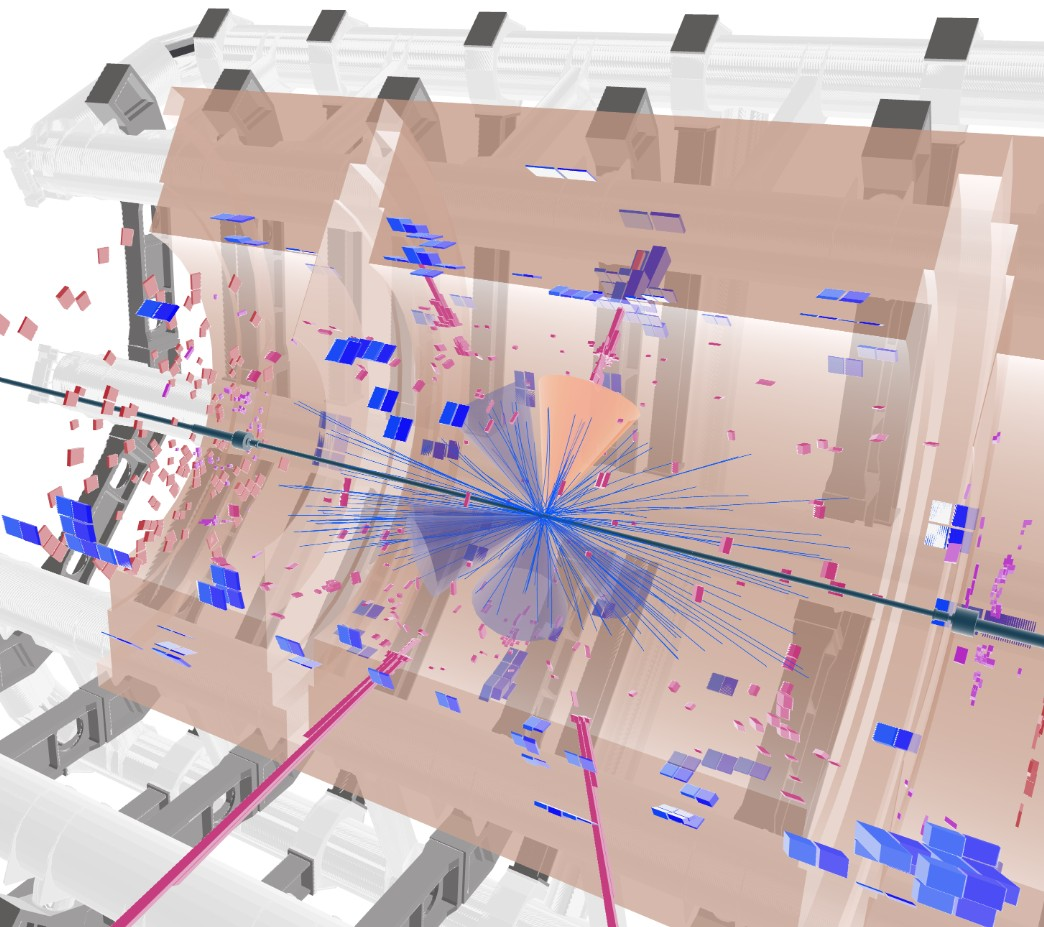
\includegraphics[width=0.4\linewidth]{figs/front2}
		\end{figure}
		
		
		\vfill
		
		
		M\"{u}nchen, 2017-2021
		
		\vspace{0.8cm}


%

		
	\end{center}
\end{titlepage}
\shipout\null
\shipout\null

\vspace*{\fill}
\noindent
{\bf Habilitation Thesis} \newline
"Search for Supersymmetry with the ATLAS detector at the LHC".\newline

\noindent
Experimental High Energy and Particle Physics.\newline

\noindent
Max-Planck-Institut f\"{u}r Physik \& Technischen Universit\"{a}t M\"{u}nchen.\newline

\noindent
M\"{u}nchen, 2017-2021.\newline

\noindent
Defended on December 12, 2019.\newline

\noindent
Submitted for reviewing in March, 2020.\newline

\noindent
Updated in November, 2021.\newline

\noindent
Final submission in February, 2022.\newline

\vspace{1cm}
\noindent
Mentoring committee:
\begin{itemize}
	\item	Prof. Dr. Hubert Kroha (Max-Planck-Institut f\"{u}r Physik, M\"{u}nchen, \textbf{Chair})
	\item	Prof. Dr. Stephan Paul (Technischen Universit\"{a}t M\"{u}nchen, \textbf{Member})
	\item 	Prof. Dr. Gregor Herten (Universit\"{a}t Freiburg, \textbf{Member})
\end{itemize}
%	\addcontentsline{toc}{section}{Acknowledgements}



\section*{Acknowledgements}

First and foremost, I would like to express my sincere gratitude to my advisor Prof. Dr. Hubert Kroha (Max-Planck-Institut f\"{u}r Physik, M\"{u}nchen) for the continuous support on my habilitation project and related research as well as for his professionalism, motivation, and immense scientific knowledge. His insightful guidance and encouragement helped me in all the time of research and completion of this effort. I could not have imagined having a better advisor and mentor for my Habilitation.

Besides my advisor, I would like to express my gratitude to the rest of my Habilitation Committee:  Prof. Dr. Stephan Paul (Technischen Universit\"{a}t M\"{u}nchen, chairman of the committee) and Prof. Dr. Gregor Herten (Universit\"{a}t Freiburg), who provided me extensive guidance to achieve the scientific goals of this thesis. Also, I am grateful to all colleagues with whom I have had the pleasure to work during this and other related projects.

A very special gratitude goes to Prof. Dr. Siegfried Bethke, director at the Max Planck Institute for Physics in Munich, for encouraging and supporting me to pursue the habilitation program.

Most importantly, I am deeply indebted  to my loving, caring and supportive wife, Louiza, and my three wonderful daughters, Marina, Arsenia and Akylina, who endlessly provide me unending inspiration.

\clearpage
\tableofcontents

\chapter{Introduction}

\section{Motivation for Supersymmetry}

For several decades, particle physicists having been trying to better understand Nature at the smallest distances by colliding particles at the highest energies. While the Standard Model (SM) of particle physics has successfully explained most of the results that have arisen from experiments, many phenomena remain baffling. 

Supersymmetry, commonly abbreviated as SUSY, is one of the most appealing extensions of the  SM.  It is a generalization of the space-time symmetries of quantum field theory that proposes a relationship between two basic classes of elementary particles: bosons, which live in an integer-valued angular momentum eigenstate (spin), and fermions, which have a half-integer spin. Each particle from one group would have an associated particle in the other, which is known as its \textit{superpartner}, the spin of which differs by a half-integer. 
\begin{figure}
	\centering
	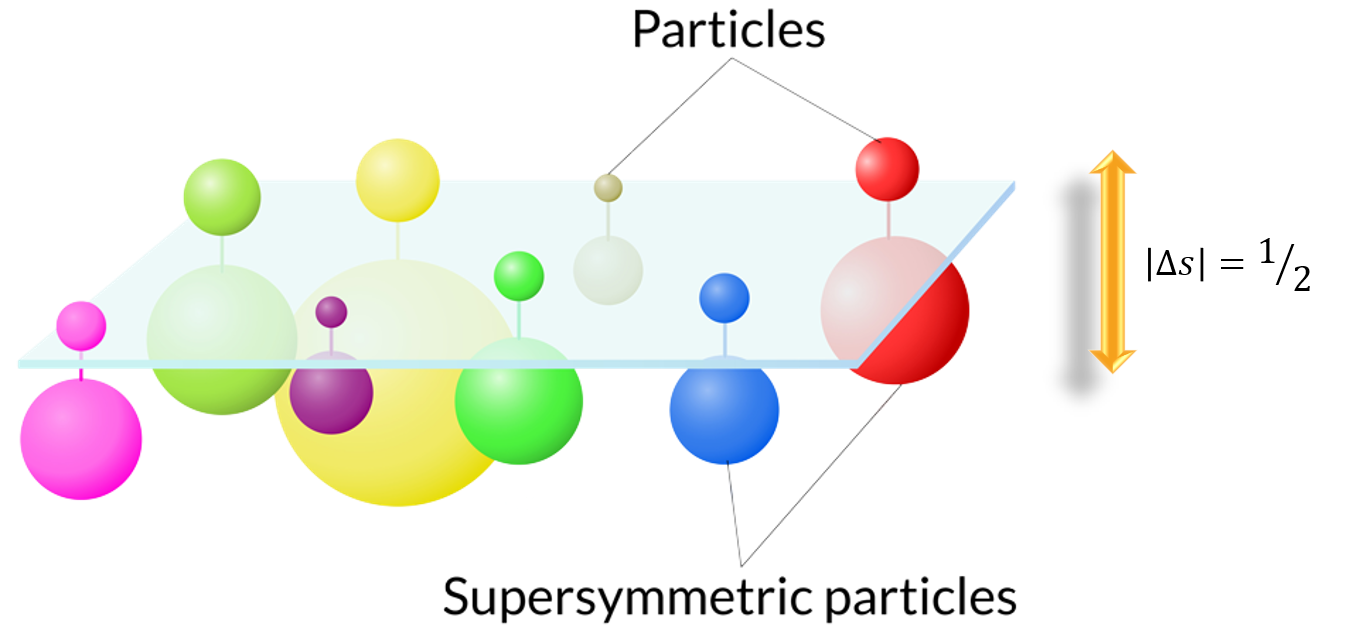
\includegraphics[width=0.7\linewidth]{figs/supersymmetry-mirror}
	\caption{SUSY comes to provide an elegant approach to provide solutions to such challenges. It is maybe the best motivated theory and compelling possible extension of SM. SUSY is a space-time symmetry that postulates the existence of new particles with \textonehalf-unit spin difference from their SM partners. For example, each SM fermion or boson is associated with a superpartner, having the same quantum numbers as its partner except for spin.}
	\label{fig:supersymmetry-mirror}
\end{figure}


There are numerous phenomenological motivations for SUSY close to the electroweak scale, as well as technical motivations for this theory at any energy scale.

First, SUSY provides a framework for the unification of particle physics and
gravity~\cite{Martin:1997ns, nath_2016, Weinberg:2000cr}
at the Planck energy scale, $M_P \sim 10^{19}~\text{GeV}$, where the gravitational interactions become comparable in magnitude to the gauge interactions. Moreover, SUSY can provide an explanation of the large hierarchy between the energy scale that characterizes electroweak symmetry breaking, $M_\text{EW} \sim 100~\text{GeV}$, and the Planck scale~\cite{Witten:1981nf, DIMOPOULOS1981150, Sakai1981, SUSSKIND1984181}.
The stability of this large gauge hierarchy with respect to radiative
quantum corrections is not possible to maintain in the  SM without an
unnatural fine-tuning of the parameters of the fundamental theory at the Planck scale. 
More specifically, in a theory such as the  SM with an elementary scalar field of mass $m$ and interaction strength $\lambda$ (e.g. the quartic scalar self-coupling; the square of a gauge coupling or the square of a Yukawa coupling), the stability with respect to quantum corrections requires the existence of an
energy cutoff roughly of order $\sqrt{ (4\pi)^2/\lambda}\;m$ beyond which new physics must enter~\cite{PhysRev.56.72}.
A significantly larger energy cutoff would require an unnatural fine-tuning of parameters
that govern the low-energy theory. Applying this argument to the  SM leads
to an expectation of new physics at the TeV scale.
In a supersymmetric extension of the  SM, thereby, it is possible to maintain
the gauge hierarchy while providing a natural framework for elementary scalar fields.

Second, the unification of the three  SM gauge couplings at a very high
energy close to the Planck scale is possible if new physics beyond the  SM
(which modifies the running of the gauge couplings above the electroweak scale) is
present. The minimal supersymmetric extension of the  SM (MSSM), where
superpartner masses lie below a few TeV, provides an example of successful gauge
coupling unification~\cite{Polonsky:2001pn}.

Third, the existence of dark matter (DM), which makes up approximately one quarter of the
energy density of the universe, cannot be explained within the  SM of particle
physics~\cite{Bertone:2004pz}.
Remarkably, a stable weakly-interacting massive particle (WIMP) whose
mass and interaction rate are governed by new physics associated with the TeV-scale
can be consistent with the observed density of dark matter, the so-called \textit{WIMP
miracle},. The lightest supersymmetric particle, if stable, is
a promising (although not the unique) candidate for the DM~\cite{PhysRevLett.48.223, ELLIS1984453, Steffen2009}.

\begin{figure}
 \centering
 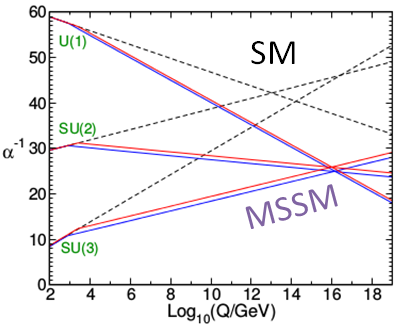
\includegraphics[width=0.6\linewidth]{figs/gut}
 \caption{Two-loop renormalization group evolution of the
  inverse gauge couplings $\alpha^{-1}_{a}(Q)\,\, a=1;\,2,\;3$ as a function of the energy scale $Q$ in the  SM (dashed
  lines) and the MSSM (solid lines). Unlike the SM, the MSSM includes just the
  right particle content to ensure that the gauge couplings can unify, at a scale $M_U \sim 1.5 \times 10^{16}~\text{GeV}$. Adapted from Ref.~\cite{Martin:1997ns}.}
 \label{fig:gut}
\end{figure}


If SUSY were an exact symmetry of nature, then particles and their superpartners would be degenerate in mass. Since superpartners have not (yet) been observed by experiments, SUSY must be a broken symmetry. Despite the break down of SUSY, the stability of the gauge hierarchy can still be maintained if the
SUSY breaking is soft~\cite{Girardello:1981wz, Jack:1999ud}, and the corresponding SUSY-breaking mass parameters are no larger than a few TeV. This, in fact, makes the search of SUSY plausible at modern collider experiments since it lies within the energy reach, for example, the Large Hadron Colllider (LHC) at CERN located in Geneva.

\section{Minimal Supersymmetric Extension of the Standard Model}
\subsection{Minimal Supersymmetric Standard Model}\label{sec:mssm}
In its minimal realization, the MSSM,  
SUSY postulates the existence of a new bosonic (fermionic) partner for each fundamental  SM fermion (boson), as well as an additional Higgs doublet. 
More specifically, electroweakly interacting supersymmetric particles are charginos, neutralinos, sleptons, sneutrinos and squarks. Charginos ($\tilde{\chi}^\pm$) and neutralinos ($\tilde{\chi}^0$) are the mass eigenstates formed by linear combinations of the superpartners of the charged and neutral Higgs bosons and of the electroweak gauge bosons. Strongly interacting superpartners are the squarks ($\tilde{q}$) and gluinos ($\tilde{g}$). 

\begin{figure}
 \centering
 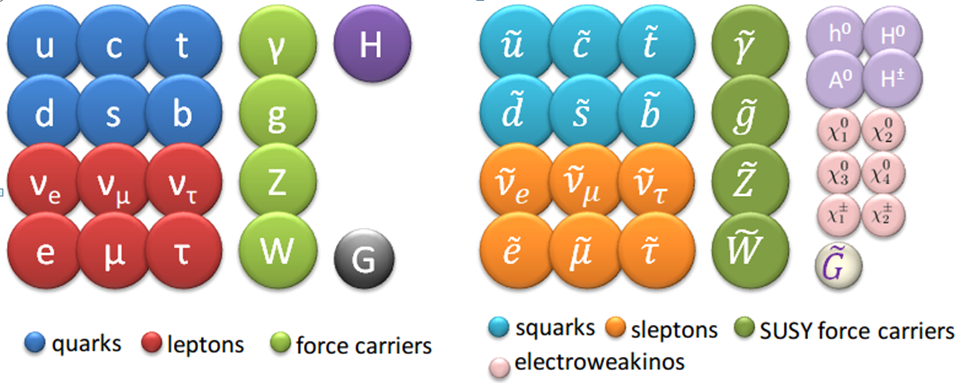
\includegraphics[width=0.85\linewidth]{figs/mssm}
 \caption{Particle content of the Minimal Supersymmetric SM theory.}
 \label{fig:mssm}
\end{figure}

The minimal supersymmetric extension of the  SM also consists of the fields of the two-Higgs-doublet extension of the  SM and the corresponding superpartners.
After electroweak symmetry breaking, five Higgs bosons arise, of
which two are charged. The supersymmetric partners of the Higgs doublets are known
as "higgsinos".
The enlarged Higgs sector of the MSSM constitutes the minimal structure needed to guarantee
the cancellation of gauge anomalies~\cite{PhysRevD.6.429}
generated by the higgsino superpartners that can appear as internal lines in triangle diagrams with three external electroweak gauge bosons. 
Moreover, without a second Higgs doublet, one cannot generate mass for both
"up"-type and "down"-type quarks, and charged leptons in a way consistent with the
underlying SUSY~\cite{Fayet:1974pd, Gunion:1984yn}.

The fact that such particles are not yet observed leads to the conclusion that, if SUSY is realized, it is a broken symmetry. A description of SUSY in the form of an effective Lagrangian
with only "soft" SUSY breaking terms and SUSY masses at the TeV scale maintains
cancellation of quadratic divergences in particle physics models

\subsection{Charginos and Neutralinos}\label{sec:ChAndNeu}
As discussed in Section~\ref{sec:mssm}, vector superfields must be introduced to describe the gauge sector. 
In particular, eight gluinos $\tilde{g}$ as partners of QCD, three winos $\tilde{W}$ as partners of the SU(2) gauge bosons, and a bino $\tilde{B}$ as
$\text{U(1)}_Y$ gaugino. 

In MSSM, the higgsinos and the electroweak gauginos mix with each other because of the effects
of electroweak symmetry breaking. Since $\text{SU}(2) \times \text{U(1)}_Y$ is broken, the winos and the bino are in general not mass eigenstates, rather they mix with fields with the same charge but different $\text{SU}(2) \times \text{U(1)}_Y$ quantum numbers.

The neutral higgsinos ($\tilde{H}_u^0$ and $\tilde{H}_d^0$) and the neutral gauginos ($\tilde{B}$ and $\tilde{W}^0$)  combine to form the mass eigenstates called \textit{neutralinos}, which are denoted by $\tilde{\chi}_i^0$ with $i=1-4$.
The charged higgsinos ($\tilde{H}_u^+$ and $\tilde{H}_d^-$) and winos ($\tilde{W}^+$ and $\tilde{W}^+$) mix to form the mass eigenstates with
electric charge $\pm 1$ called \textit{charginos}, which are denoted by $\tilde{\chi}_i^\pm$ with $i=1,\,2$.
By convention, these mass eigenstates are labelled in ascending mass order, so that $m_1 < \cdots < m_4$ for neutralinos and $m_1 < m_2$ for charginos.
The lightest neutralino, $\tilde{\chi}_1^0$, is typically assumed to be the LSP, unless there is a lighter gravitino, or unless R-parity
is not conserved, because it is the only MSSM particle that can make a good dark matter candidate.

In the gauge interaction eigenstate basis, the neutralino and chargino can be expressed as $\psi^0 = (\tilde{B},\, \tilde{W},\, \tilde{H}_d^0,\, \tilde{H}_u^0)$
and $\psi^\pm = (\tilde{W}^+,\, \tilde{H}_u^+,\, \tilde{W}^-,\, \tilde{H}_d^-)$, respectively.
To obtain mass eigenstates, a unitary mixing matrix is used to diagonalize the mass matrix. The mass eigenvalues and the mixing matrix can be then given in closed form in
terms of the parameters $M_1$, $M_2$, $\mu$ and $\tan\beta$.
The parameters $M_1$ (bino mass term) and $M_2$ (wino mass term) come directly from the MSSM soft Lagrangian, 
while $\mu$ has dimension of mass, corresponding to a mass term mixing the 2 Higgs doublets. This parameter can be either positive or negative.
The parameter $\tan\beta$ is defined as the ratio of the two vacuum expectation values, $\nu_u / \nu_d$, of the two Higgs doublets.

There is a not-unlikely limit in which electroweak symmetry breaking effects can be viewed as a
small perturbation on the neutralino mass matrix. If 
\begin{equation}\label{eq:mz-limit}
m_Z \ll |\mu \pm M_1|,\, |\mu\pm M_2|
\end{equation}
then the neutralino mass eigenstates are very nearly a "bino-like" $\tilde{\chi}_1^0 \approx \tilde{B}$, a "wino-like" $\tilde{\chi}_2^0 \approx \tilde{W}^0$ and 
"higgsino-like" $\tilde{\chi}_3^0,\,\tilde{\chi}_4^0 \approx (\tilde{H}_u^0 \pm \tilde{H}_d^0)/\sqrt{2}$.
In the same limit of Equation~\ref{eq:mz-limit}, the chargino mass eigenstates consist of "wino-like" $\tilde{\chi}_1^\pm$ and a higgsino-like $\tilde{\chi}_2^\pm$.

\subsection{Squarks and Gluinos}
The squarks are the scalar superpartners of the quarks and there is one version for each SM quark. 
Due to phenomenological constraints from flavor changing neutral currents (FCNC), 
typically the lighter two generations of squarks have to be nearly the same in mass.
The superpartners of the top and bottom quark can be separated from the lighter squarks and are called stop and sbottom.
Squarks can be produced through strong interactions and therefore are easily produced at hadron colliders such as the LHC. 
They decay to quarks and neutralinos or charginos which can further decay. 

Gluinos are Majorana fermionic partners of the gluon, which means that they are their own antiparticles. They interact strongly and therefore can be produced significantly at the LHC. 
The decay of the gluino can only proceed through a squark, either on-shell or virtual.
In case of two-body, gluino decays to quark-squark pairs they will dominate as the relevant gluino-quark-squark coupling has QCD strength. If the the top and bottom squarks are lighter than all of the other squarks, it is possible that gluino decays to either top-stop or bottom-sbottom are the only available two-body decay modes, in which case they will dominate over all others.
If instead all of the squarks are heavier than the gluino, the gluino will decay only through off-shell squarks giving rise to 3-body decays involving neutralinos and charginos, i.e. $\tilde{g} \to qq\; \tilde{\chi}_i^0$ or $q^\prime q\; \tilde{\chi}_i^\pm$.

\subsection{Sleptons}

Sleptons are the scalar partners of the leptons of the Standard Model. 
They are not strongly interacting and therefore are often produced with lower cross-section at hadron colliders unless they are very light.
Because of the high mass of the tau lepton, there will be left-right helicity mixing of the stau similar to that of stop and sbottom.
Sleptons will typically be found in decays of a charginos and neutralinos if they are light enough to be a decay product.

\section{R-Parity}
In the absence of a protective symmetry, SUSY processes violating the lepton ($L$) and baryon ($B$) quantum numbers result in proton decay at a rate that is in conflict with the experimental constraints on its lifetime. This conflict can be avoided by imposing a $B-L$  conservation requirement on the supersymmetric Lagrangian when defining the MSSM.  As a consequence of the $B-L$ symmetry, the MSSM possesses a multiplicative R-parity invariance, which is defined as
\begin{equation}
R = (-1)^{3(B-L)+2S}
\end{equation}
for a particle of spin S~\cite{FARRAR1978575}. This implies that all the particles of the  SM have even R-parity, whereas the corresponding
superpartners have odd R-parity. 
\begin{figure}[htbp]
	\centering
	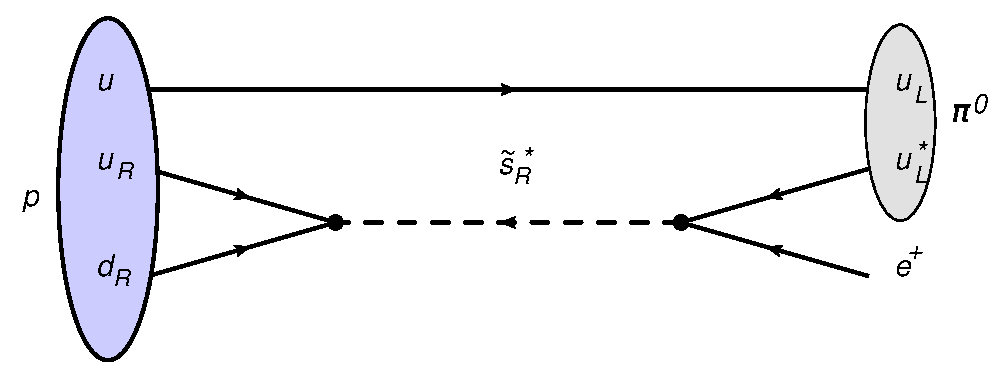
\includegraphics[width=0.5\linewidth]{figs/p-decay}
	\caption{Proton decay into a positron and a neutral pion: $p \rightarrow \pi^0 \; e^+$.}
	\label{fig:p-decay}
\end{figure}


The conservation of R-parity in scattering and decay processes has a critical impact on supersymmetric phenomenology. For example, any initial state in a scattering experiment will involve ordinary (R-even) particles. Consequently, it follows that supersymmetric particles must be produced in pairs. 
In general, these particles are highly unstable and decay into lighter states.
R-parity invariance also implies that the lightest supersymmetric particle (LSP) is
absolutely stable, and must eventually be produced at the end of a decay chain initiated
by the decay of a heavy unstable supersymmetric particle.
In order to be consistent with cosmological constraints, a stable LSP is certainly
electrically and color neutral~\cite{ELLIS1984453}. Therefore, the LSP in an R-parity-conserving (RPC) theory is weakly interacting with ordinary matter, i.e., it behaves like a stable heavy neutrino and will escape collider detectors without being directly observed. Thus, the canonical signature for conventional RPC supersymmetric theories is substantial missing (transverse) energy, due to the LSP escaping from any detection means. Finally, the stability of the LSP in RPC SUSY makes it a promising candidate for dark matter.

If R-parity is violated, new lagrangian terms parameterized by $\lambda_{ijk}$,  $\lambda_{ijk}^\prime$  and  $\lambda_{ijk}^{\prime\prime}$ appear in the superpotential, where $ijk$ are particle generation indices. 
\begin{equation}
W =  \lambda_{ijk} \mathrm{L}_i  \mathrm{L}_j   \bar{\mathrm{E}}_k
+  \lambda_{ijk}^\prime  \mathrm{Q}_i  \mathrm{L}_j   \bar{\mathrm{D}}_k
+  \lambda_{ijk}^{\prime\prime}  \bar{\mathrm{U}}_i  \bar{\mathrm{D}}_j   \bar{\mathrm{D}}_k
+ m_i \mathrm{L}_i  \mathrm{H}_u
\end{equation}
where Q, U, D, L, E  are the matter superfields and $\mathrm{H}_{u,d}$ are the up and down type Higgs superfields.
The $\lambda$-type couplings appear between lepton superfields only, $\lambda^{\prime}$-type are between quark superfields only, and $\lambda^{\prime\prime}$-type couplings
connect the two. R-parity violation (RPV) implies lepton and/or baryon number violation. 
In this case, the lightest neutralino can decay even if it is the LSP. If the decay involves a non-zero $\lambda$ coupling, the final state will be a multi-lepton one.
Searches for events with four or more isolated charged
leptons by the ATLAS~\cite{ATLAS-CONF-2015-018, ATLAS-CONF-2016-075, Aaboud:2018zeb} 
and CMS~\cite{CMS-PAS-SUS-13-010} 
experiments are interpreted in such models. The search of multi-lepton final states and interpretation in SUSY RPV models is subject of this thesis.
With very small coupling values, the neutralino would be long-lived, leading to lepton pairs with a
displaced vertex, which have also been searched for~\cite{PhysRevD.92.072004, CMS:2015pca}.

\section{Naturalness and Light Higgsinos}\label{sec:Naturalness}
While the SM provides an excellent description of most experimental data, it is known to be highly unnatural in the scalar (Higgs) 
sector if its regime of validity as an effective theory is taken much beyond the $\Lambda \sim 1$~TeV energy scale. 
Many solutions to the SM naturalness problem have been invoked. However, in the SUSY theory, quadratic divergences 
cancel to all orders in perturbation theory, rendering the theory \textit{natural}.

Recent searches at LHC with $\sqrt{s} = 13$~TeV proton-proton collision data, exclude, within the context of various simplified models,
the squark and gluino production beyond the TeV mass scale (see Figure~\ref{fig:susysum}).
In addition, the measured value of the Higgs mass at $m_h \simeq 125.2$~GeV seems to require highly mixed TeV-scale top-squarks. 
These various mass bounds are in deep discord from early naturalness constraints, this time mainly arising from logarithmic rather than quadratic divergences.

The most direct relation between the observed value of the weak scale and elements of the SUSY Lagrangian comes from minimizing the MSSM scalar potential. 
It is found that
\begin{equation}\label{eq:mz2}
\frac{m_Z^2}{2} = \frac{m_{H_d}^2 + \Sigma_d^d - (m_{H_u}^2 + \Sigma_u^u) \, \tan^2\beta}{\tan^2\beta-1} -\mu^2 \simeq  -m_{H_u}^2 - \Sigma_u^u - \mu^2
\end{equation}
where $\tan\beta \equiv \nu_u / \nu_d$ is the ratio of Higgs field vacuum expectation values, $m_{H_d}^2$ and $m_{H_u}^2$ the field soft SUSY breaking terms
 and $\mu$ is the superpotential Higgs/higgsino mass term.
 If any term on the right-hand-side is far greater than $m_Z^2/2$, then some other term would
have to be fine-tuned to an opposite-sign value such as to maintain $m_Z$ at its measured value.
Alternatively, for a natural theory, all terms on the right-hand side of Equation~\ref{eq:mz2} should be comparable to or smaller
than  $m_Z^2/2$. The electroweak fine-tuning measure $\Delta_\mathrm{EW}$ was introduced~\cite{PhysRevLett.109.161802} to measure the
largest contribution on the right-hand side of Equation~\ref{eq:mz2} compared to $m_Z^2/2$. 
For a natural theory with low $\Delta_\mathrm{EW}$, one finds that the soft parameter $m_{H_u}^2$ is driven radiatively
to small negative values at the weak scale. Also, in order that the radiative corrections $\Sigma_u^u\lesssim m_Z^2/2$,
the top-squarks are highly mixed and not too far beyond the few TeV range. 
The latter requirement is completely consistent with the measured value of $m_h$ and with expectations from
the measured decay rate of the process $b \to s \gamma$. 
In addition, the gluino mass feeds into the  $\Sigma$ radiative terms and thus $m_{\tilde{g}} < 4$~TeV.
 Finally, for $\mu \sim  100-300$~GeV, the closer to $m_Z$ the better for naturalness.

This latter condition implies the existence of four higgsino-like states $\tilde{\chi}_1^\pm/\tilde{\chi}_2^0/\tilde{\chi}_1^0$ 
with mass in the range 100-300 GeV (the closer to Z boson mass, the better). 
Higgsinos are the only SUSY particles required to be near the weak scale. 
These particles are difficult to be detected at LHC due to their compressed spectra:  the lightest higgsino-like electroweakino  is typically just
5-20 GeV lighter than the heavier ones.
Since $\tilde{\chi}_1^0$ would constitute a candidate of the dark matter, the bulk of energy produced from higgsino decays becomes bound
up in the $\tilde{\chi}_1^0$  mass. 

Consequently, the lightest state is totally invisible while the heavier states lead only to soft particles, such as very low-$\pt$ charged leptons and jets, which are difficult to distinguish from QCD and other SM backgrounds.

\section{Phenomenology of Supersymmetry}
The phenomenology of SUSY is to a large extent determined by the SUSY breaking mechanism and the SUSY breaking scale. This determines the SUSY particle masses, the mass hierarchy, the field contents of physical particles, and their decay modes. 
In addition, phenomenology crucially depends on whether the multiplicative quantum number of R-parity is conserved or violated. In most cases, supersymmetric events are characterized by a high multiplicity of final state particles and a large amount of missing transverse energy due to the undetected LSP and possible production of neutrinos.

Since the mechanism by which SUSY is broken is unknown, a general approach to
SUSY via the most general soft SUSY breaking Lagrangian adds a significant number
of new free parameters. For the MSSM, these comprise 105 new parameters. A
phenomenological analysis of SUSY searches leaving all these parameters free is not
feasible. For the practical interpretation of SUSY searches at colliders, several approaches are taken to reduce the number of free parameters. The most common approach is to assume a SUSY breaking mechanism and lower the number of free parameters through the assumption of additional constraints, such the R-parity conservation or not, the particle masses and decay branching ratios.

At the LHC, most searching approaches are developed to increase the sensitivity to pair production of heavy sparticles with TeV-scale masses focusing on the kinematics of their decays, and to further suppress the background from  SM processes.

Selection variables designed to separate the SUSY signal from the SM backgrounds typically include $H_\mathrm{T}$, $E_\mathrm{T}^\text{miss}$, and $m_\text{eff}$. The reconstructed quantities  $H_\mathrm{T}$ and $E_\mathrm{T}^\text{miss}$
refer to the measured transverse energy and missing transverse momentum in the event, respectively. They are defined as the scalar sum of the transverse particle momenta or calorimeter clusters transverse energies measured in the event ($H_\mathrm{T}$), or the negative vector sum of transverse momenta of reconstructed objects like jets and leptons in the event ($E_\mathrm{T}^\text{miss}$). The event observable  $m_\text{eff}$ is referred to as the effective mass of the event and is defined as the sum of $H_\mathrm{T}$ and $E_\mathrm{T}^\text{miss}$. The peak of the  $m_\text{eff}$  distribution for SUSY signal events correlates with the SUSY mass scale, in particular with the mass difference between the primary produced SUSY particle and the LSP, whereas the  SM backgrounds
typically dominate at low $m_\text{eff}$ values.  Additional reduction of multijet backgrounds can be achieved by requiring isolated leptons or photons in the final states.

Recently, alternative approaches have been developed to increase the sensitivity
to pair production of heavy sparticles with TeV-scale masses focusing on the kinematics
of their decays, and to further suppress the background from multijet production.
Prominent examples of these new approaches are searches using the $\alpha_T$ variable~\cite{PhysRevLett.101.221803, Chatrchyan:2013mys},
\textit{razor} variables~\cite{Chatrchyan:2012lia}, \textit{stransverse mass}  ($m_{\mathrm{T}2}$)~\cite{Lester:1999tx},
and contransverse mass ($m_{\mathrm{CT}}$)~\cite{Tovey:2008ui}. 
In particular, a lower bound on the stransverse mass can be imposed in event selections to reduce contributions from $t\bar{t}$ and $WW$ events.
The $m_{\mathrm{T}2}$ variable is defined as:
\begin{equation}\label{eq:mt2}
m_{\mathrm{T}2} = \min_{\mathbf{q}_\mathrm{T}}\left[\max\left(m_{{\mathrm T}}^{(1)}(\mathbf{p}_{\mathrm{T}}^{(1)},\, \mathbf{q}_\mathrm{T}),m_{\mathrm T}^{(2)} (\mathbf{p}_{\mathrm{T}}^{(2)},\mathbf{E}_\mathrm{T}^\mathrm{miss}-\mathbf{q}_\mathrm{T})\right)\right],
\end{equation}
where $\mathbf{p}_{\mathrm{T}}^{(i)}, \; i =1,\;2$ are the transverse momenta of a reconstructed particle pair, and $\qTvec$ is the transverse momentum vector that minimizes the larger of the
two transverse masses $m_{{\mathrm T}}^{(i)},\, \; i =1,\;2$.
The latter masses are defined by
\begin{equation}
m_{{\mathrm T}}(\pTvec,\, \mathbf{q}_\mathrm{T}) = \sqrt{2(p_\mathrm{T}\qT-\pTvec\cdot \mathbf{q}_\mathrm{T})}\; .
\end{equation}
For $t\bar{t}$  and $WW$ events, in which two $W$ bosons decay leptonically and $\mathbf{E}_\mathrm{T}^\mathrm{miss}$
is the sum of the transverse momenta of the two neutrinos, the $m_{\mathrm{T}2}$ distribution has a kinematic end-point at the $W$ mass. For large mass differences between the staus and the lightest neutralino, the $m_{\mathrm{T}2}$ distribution for signal events extends significantly beyond this end-point.


Furthermore, the topological event reconstruction methods have expanded with the \textit{superrazor}~\cite{Buckley:2013kua}
and \textit{recursive jigsaw reconstruction}~\cite{PhysRevD.96.112007} techniques. 
Finally, the searches including massive SUSY particles attempt to identify their decay into top quarks or vector bosons, which are themselves unstable. If these are produced with a significant boost, jets(tau lepton) from their decay will typically overlap, and such topologies are searched for with jet(tau lepton)-\textit{substructure} techniques~\cite{PhysRevLett.100.242001}.

\section{Experimental Search Program for SUSY}
Searches for SUSY and new physics in general were part of the physics program of large collider experiments, such as the LEP electron-positron collider at CERN, the Tevatron proton-antiproton collider at Fermilab, the HERA electron-proton collider at DESY, and the LHC proton-proton ($pp$) collider at CERN.

Searches for new physics at $e^+e^-$ colliders benefit from the clean experimental
environment and the fact that momentum balance can be measured not only in the plane
transverse to the beam, but also in the direction along the beam pipe, defined as the longitudinal direction. Searches at LEP are dominated by the data
samples taken at the highest center-of-mass energies.
On the other hand, proton-(anti)proton colliders produce interactions at higher center-of-mass energies than those available at LEP, and cross sections of QCD-mediated processes are larger, which is reflected in the higher sensitivity for SUSY particles carrying color charge: squarks and gluinos. Large background contributions from  SM processes, nonetheless, pose challenges to data acquisition and analysis. Such backgrounds are dominated by QCD multijet production processes, the top quark production, as well as jet production in association with vector gauge bosons. The proton momentum is shared between its parton constituents, and in each collision only a fraction
of the total center-of-mass energy is available in the hard parton-parton scattering.
Since the parton momenta in the longitudinal direction are not known on an event-by-event
basis, use of momentum conservation constraints in an analysis is restricted to the
transverse plane, leading to the definition of transverse variables, such as the missing
transverse energy $E_\mathrm{T}^\text{miss}$, and the transverse mass $m_\mathrm{T}$.

Today, there is no evidence to show whether or not SUSY is correct, or what other extensions to current supersymmetric models might be more accurate. Despite this, SUSY is being supported by physicists since it remains the most complete theory to describe possible phenomena beyond the SM. 
%
Low-energy data from flavor physics experiments, high-precision electroweak
observables as well as astrophysical data impose strong constraints on the allowed
SUSY parameter space. 
Recent examples of such data include measurements of the rare B-meson decay 
$B_s \to \mu^+ \mu^-$~\cite{Oyanguren:2018huo, PhysRevLett.118.191801}, measurements of the anomalous magnetic moment
of the muon~\cite{Czarnecki:2000id}, and accurate determinations of the cosmological dark matter relic density constraint~\cite{Ade:2015xua}.

These indirect constraints are often more sensitive to higher SUSY mass scales than
experiments searching for direct sparticle production at colliders, but the interpretation of
these results is often strongly model dependent.
%
On the other hand, direct confirmation would entail production of superpartners in collider experiments, such as the LHC. 
Direct searches for sparticle production at collider experiments are less subject to interpretation ambiguities and therefore they play a crucial role in the search for SUSY.

The first runs of the LHC found no previously-unknown particles other than Higgs boson with a mass around 125 GeV, which was already suspected to exist as part of the  SM. With the discovery of the Higgs boson, further constraints were imposed on a plethora of SUSY models~\cite{PhysRevD.98.030001}.


\section{Scope of Thesis}

This habilitation thesis attempts to cover searches from the electroweak sector of SUSY, mostly involving leptons in the final state. The electroweak processes are characterized by a very small production cross-section, at minimum one order of magnitude less than those processes involving the strong force, as presented by Figure~\ref{fig:xsec1}. Due to exactly the colored production of gluinos and squarks, the SUSY partners of gluons and quarks, hadron collider experiments are able to set much tighter mass limits.
\begin{figure}[htbp]
 \centering
 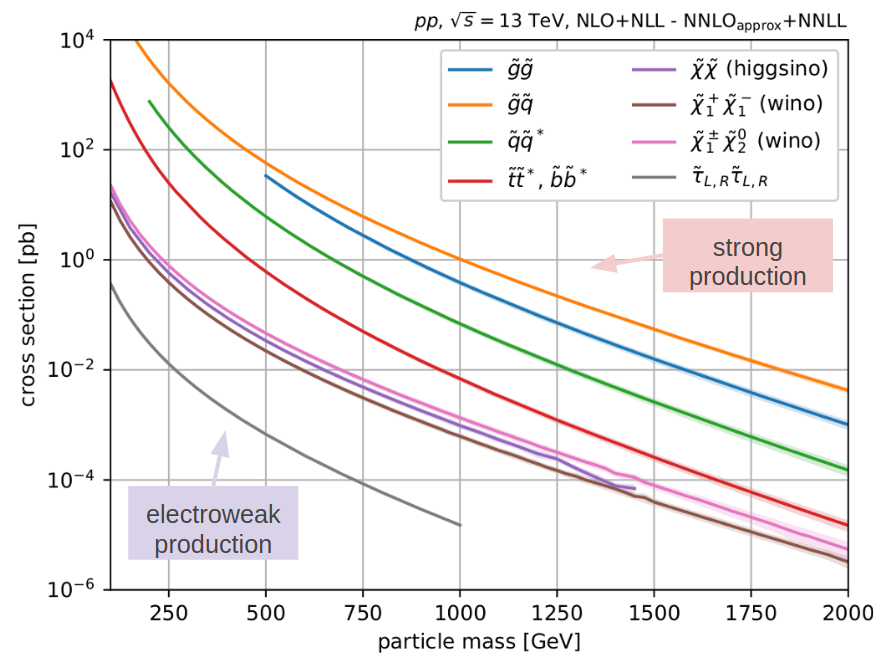
\includegraphics[width=0.8\linewidth]{figs/xsec1}
 \caption{Cross sections for pair production of different SUSY production modes as a
  function of the sparticle mass at the LHC for a center-of-mass energy of 13~TeV.
  The cross section of pair production of electroweak gauginos at the LHC, for masses of several hundreds of GeV, is at least two orders of magnitude smaller than for colored SUSY particles (e.g. top squark pair production). Adapted from Ref.~\cite{susy:xsec}.
 }
 \label{fig:xsec1}
\end{figure}
Despite this fact, the search for SUSY in electroweak scenarios is also feasible due the distinct signal signatures in the event final state which suppress significantly the SM background sources.
For example, the search of multileptonic final states requires the presence many leptons in the event, and the search of direct production of tau sleptons require high values of the $m_\text{eff}$ observable. Both selection requirements reduce significantly the SM processes that mimic these SUSY signal events.
The search of these SUSY scenarios consist the main topic of this thesis, which presents the methodology and discusses the main results. Since none of the searches performed so far have shown significant excess above the  SM background prediction, the interpretation of the presented results is focused on showing exclusion limits on the SUSY parameter space.

In the following, the ATLAS detector at the LHC is shortly described. Then, the main ingredients of the analysis structure and result interpretation are presented, as well as the conclusions of each search. Whereas necessary, the assumptions that have entered the limits when quoting interpretations from simplified models will be explicitly pointed out. The papers accepted for publication or already published in electronic journals are enclosed in the Appendix~\ref{ch:app-b}.


\chapter{ATLAS Detector}
The ATLAS detector~\cite{ATLAS_2008}, shown in Figure~\ref{fig:atlas}, is a multipurpose particle detector with a forward-backward symmetric cylindrical
geometry and nearly $4\pi$ coverage in solid angle.
\begin{figure}[htbp]
 \centering
 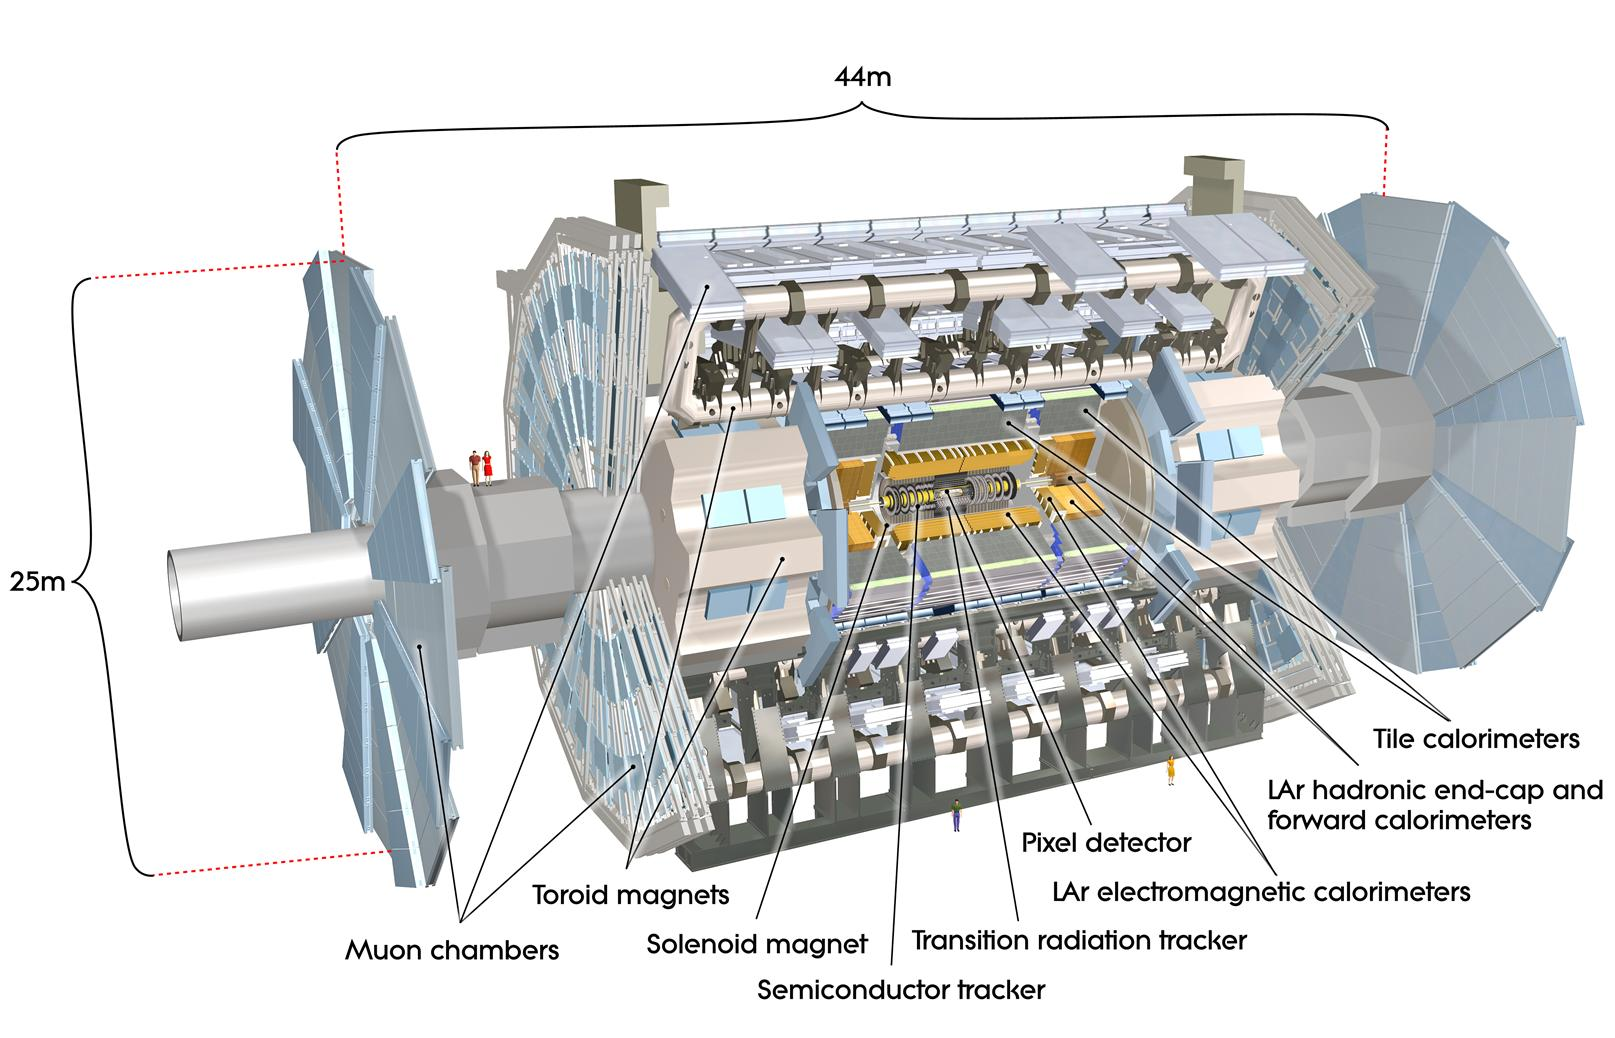
\includegraphics[width=0.9\linewidth]{figs/atlas}
 \caption{Cutaway drawing of the ATLAS detector showing its main detection components.}
 \label{fig:atlas}
\end{figure}
The entire detector weighs approximately 7,000 tons, and is 44 m long and 25 m in diameter. It is situated in an underground cavern at a depth of 100 m, where it surrounds one of the collision points around the 27-km-long LHC ring. The first $pp$ collisions at the LHC were recorded in 2009, and since then collider has operated at different center-of-mass-energies, namely 7, 8 and 13~TeV.
\begin{figure}
	\centering
	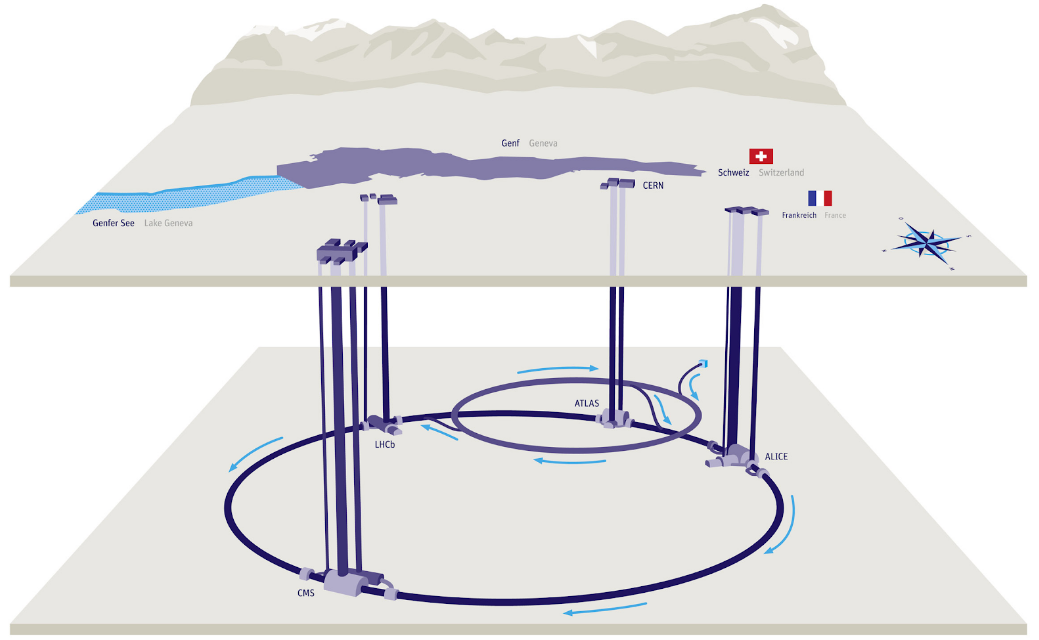
\includegraphics[width=1.0\linewidth]{figs/lhc}
	\caption{The Large Hadron Collider accelerator complex at CERN; the world's largest and highest-energy particle collider and the largest machine in the world. First collisions were achieved in 2010 at an energy of 3.5~TeV per beam. After upgrades it reached 6.5~TeV per beam. The design luminosity of the LHC is $10^{34}\;\text{Hz}\;\text{cm}^{-2}$, which was first reached in June 2016. By 2017, twice this value was achieved.
	Colliding protons are bunched together, into up to 2808 bunches, with 115 billion protons in each bunch so that interactions between the two beams take place at discrete intervals, mainly 25~ns apart, providing a bunch collision rate of 40~MHz.}
	\label{fig:lhc}
\end{figure}


\section{Coordinate System}
ATLAS uses a right-handed coordinate system with its origin at the nominal interaction point (IP) in the center of the detector and the z-axis along the beam pipe. The x-axis points from the IP to the center of the LHC ring, and the y-axis points upward. 
Cylindrical coordinates $(r,\, \phi)$ are used in the transverse plane, $\phi$ being the azimuthal angle around the z-axis. Pseudorapidity, $\eta$, is defined in terms of the polar angle $\theta$ as $\eta = - \ln \tan(\theta/2)$. Rapidity is defined as $y = 0.5 \ln (E + p_z )/(E - p_z )$
where $E$ denotes the energy and $p_z$ is the component of the momentum along the beam direction.

\section{Inner Detector}
The inner tracking detector (ID) consists of silicon pixel detector and semiconductor tracker (SCT) detectors covering the pseudorapidity region $|\eta| < 2.5$. These systems are surrounded by a transition
radiation tracker (TRT), which enhances electron identification in the region $|\eta| < 2.0$. 
Before LHC Run 2, a new innermost pixel layer, the insertable B-layer~\cite{CERN-LHCC-2012-009}, was inserted at a mean sensor radius of $3.3$~cm. 
\begin{figure}[thbp]
 \centering
 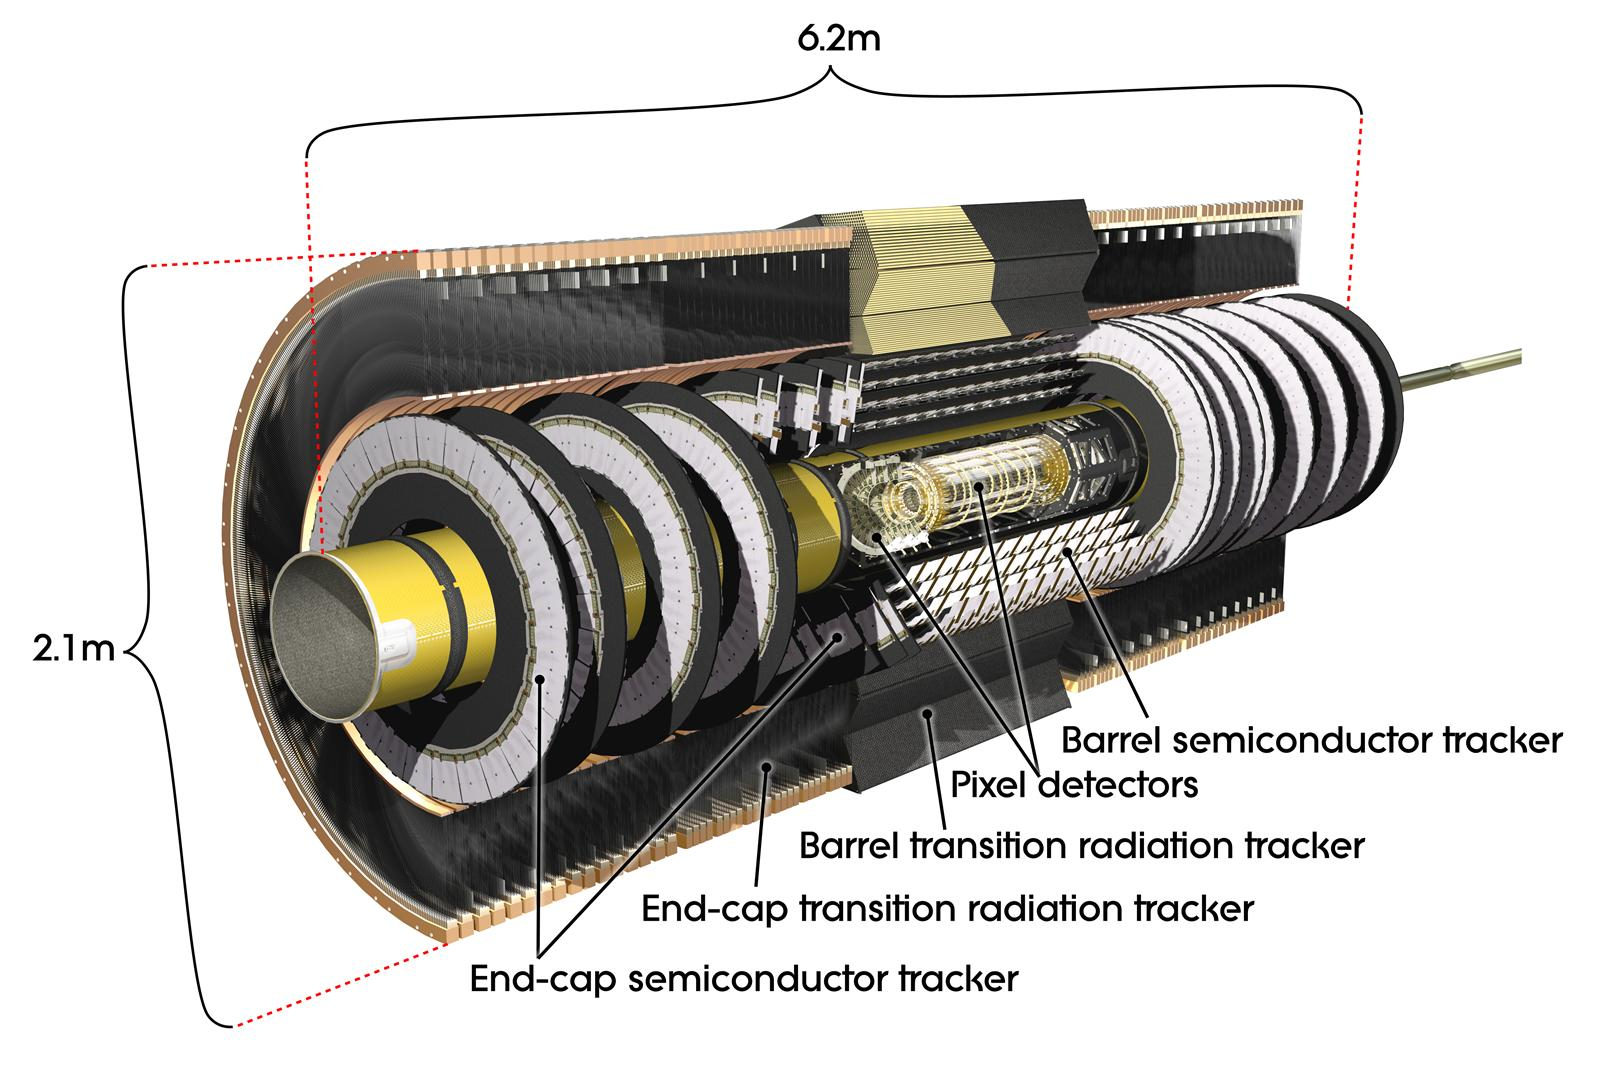
\includegraphics[width=0.7\linewidth]{figs/id}
 \caption{Cut-away image of the ATLAS Inner Detector.}
 \label{fig:id}
\end{figure}
The ID is surrounded by a thin superconducting solenoid providing an axial 2~T magnetic field.

\section{Calorimeters}
A fine granularity lead/liquid-argon (LAr) electromagnetic (EM) calorimeter, covering $|\eta| < 3.2$, is used to reconstruct electrons and photons.
A steel/scintillator tile calorimeter provides coverage for hadronic showers in the central pseudorapidity range ($|\eta| < 1.7$).

The endcaps ($1.5 < |\eta| < 3.2$) of the hadronic calorimeter have LAr active layers with either copper
or tungsten as the absorber material. The forward region ($3.1 < |\eta| < 4.9$) is instrumented with a LAr
calorimeter for both the EM and hadronic measurements. 

\section{Muon Spectrometer}

The ATLAS muon spectrometer (MS) is cylindrical, 22~m in diameter and 45~m in length, surrounding the
calorimeters with an acceptance coverage of $2\pi$ in azimuth and $\pm 2.7$ in pseudorapidity.
It is designed to detect muons in the pseudorapidity region
up to $|\eta| = 2.7$, and to provide momentum measurements with a relative resolution $\delta p /p$ better than 3\% over a wide  $p_T$ range and up to 10\% at $p_T \simeq 1$~TeV~\cite{Aad:2016jkr}. 

The MS consists of one barrel ($|\eta| < 1.05$) and two endcap sections ($1.05 < |\eta| < 2.7$). 
A system of three large superconducting air-core toroidal magnets, each with eight coils, provides a magnetic field with a bending integral  $B \cdot dl$ of about $2.5~\mathrm{T}\cdot \mathrm{m}$ in the barrel and up to $6~\mathrm{T}\cdot \mathrm{m}$ in the endcaps. 
Resistive plate chambers (RPC, three doublet layers for $|\eta| < 1.05$) and thin gap chambers
(TGC, one triplet layer followed by two doublets for $1.0 < |\eta| < 2.4$) provide triggering capability to the detector as well as $(\eta,\; \phi)$ position measurements with typical spatial resolution of $5 - 10~\text{mm}$. 
A precise momentum measurement for muons with pseudorapidity up to $|\eta| = 2.7$ is provided by three layers of monitored drift tube chambers (MDT), with each chamber providing six to eight $\eta$ measurements along the muon trajectory. 
For $|\eta| > 2$, the inner layer is instrumented with a quadruplet of cathode strip chambers (CSC) instead of MDTs. 
The single-hit resolution in the bending plane for the MDT and the CSC is about $80~\mu\mathrm{m}$ and $60~\mu\mathrm{m}$, respectively. 
The muon chambers are aligned with a precision between $30~\mu\mathrm{m}$ and $60~\mu\mathrm{m}$.


%
\begin{figure}[hbtp]
 \centering
 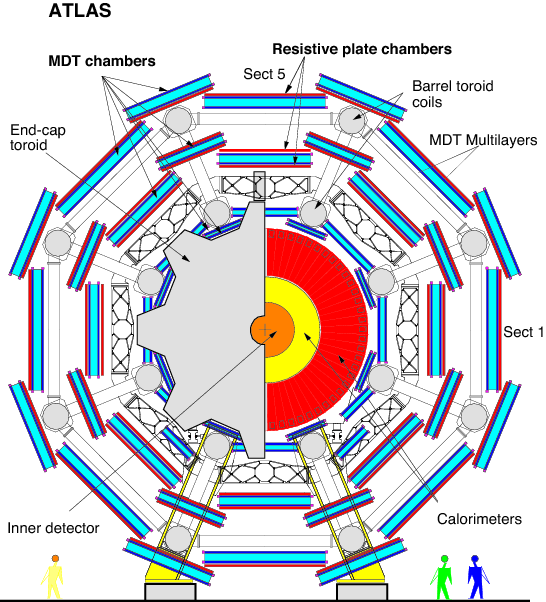
\includegraphics[width=0.45\linewidth]{figs/muons}
 \caption{Cross-sectional view of the ATLAS muon spectrometer.}
 \label{fig:muons}
\end{figure}
%


\section{Trigger System}
The ATLAS trigger system~\cite{Aaboud:2016leb} consists of a hardware-based level-1 (L1) trigger followed by a software-based high-level trigger (HLT). 

The L1 hardware trigger is constructed with custom-made electronics and runs with a fixed latency of $2.5~\mu\mathrm{s}$. It works on a subset of information from the calorimeter and muon detectors. The decision to keep the data from an event is made less than two-and-half microseconds after the event occurs, and the event is then retrieved from pipelined storage buffers. The L1 trigger reduces substantially the event rate from the LHC interaction rate of 40 MHz, and can save at most 100~k events per second for the HLT. 

The HLT software trigger-based trigger is assembled by a large farm of CPUs and serves to refine the analysis of the L1 trigger. In the HLT, offline-like reconstruction algorithms run in a large farm of  $\sim 40$k processor cores and a decision is formed typically within 300~ms. It conducts a very detailed analysis either by performing overall examination of the whole event for selected layers of the detector (for example calorimeters, trackers, muon detectors), or, by utilizing the data in smaller and isolated regions of the detector. About 1k events per second are selected by the HLT analysis and are fully assembled into an event record. These events are finally passed on to a data storage system for offline analysis.

\section{Luminosity}
A precise measurement of the integrated luminosity is a key component of the ATLAS physics program, in particular for cross-section measurements where it is often one of the leading sources of
uncertainty~\cite{ATLAS-CONF-2019-021}. The luminosity measurement is based on an absolute calibration of the primary luminosity-sensitive detectors in low-luminosity runs with specially-tailored LHC conditions using the van der Meer (vdM) method~\cite{GRAFSTROM201597}. 
The total uncertainties on the integrated luminosity measurements  for each individual year of data-taking range from 2.0 to 2.4\%, and are partially correlated between years.

Figures~\ref{fig:intlumivsyear} and \ref{fig:intlumivstimerun2dqall} presents the cumulative luminosity versus day delivered to ATLAS during stable beams and for high energy $pp$ collisions.
\begin{figure}
 \centering
 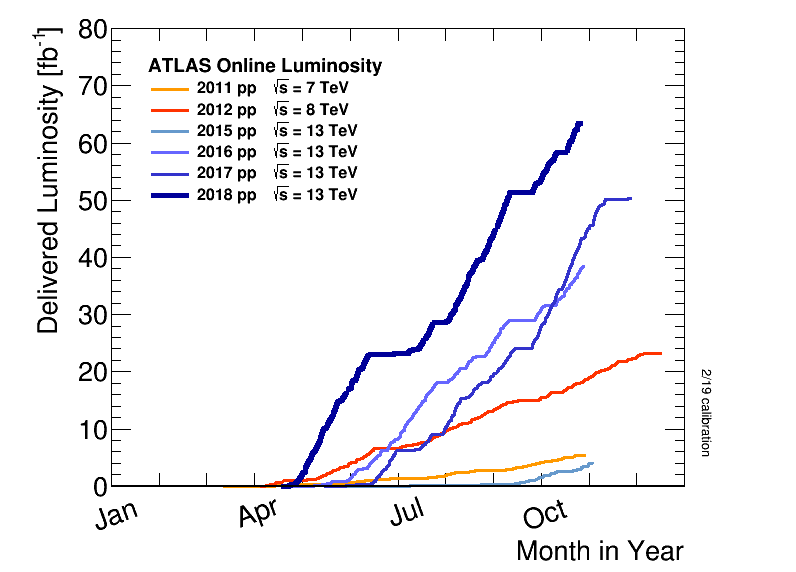
\includegraphics[width=0.75\linewidth]{figs/intlumivsyear}
 \caption{Delivered luminosity to ATLAS for $pp$ collisions versus time for years 2011-2018~\cite{lumi-atlas}.}
 \label{fig:intlumivsyear}
\end{figure}
After typical data-quality selections, the full Run 2 $pp$ data sample corresponds to an integrated luminosity of $139~\mathrm{fb}^{-1}$, with an uncertainty of 1.7\%.

\begin{figure}
	\centering
	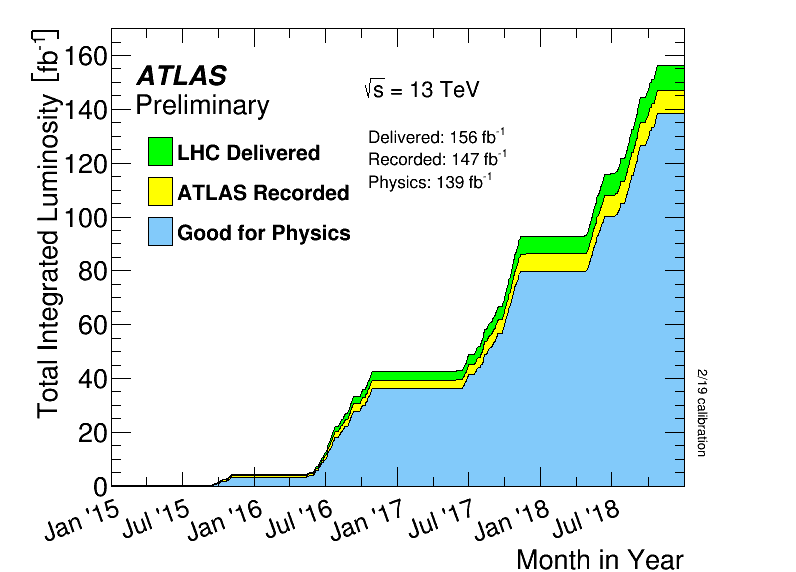
\includegraphics[width=0.75\linewidth]{figs/intlumivstimeRun2DQall}
	\caption{Cumulative luminosity versus time delivered to ATLAS (green), recorded by ATLAS (yellow), and certified to be good quality data (blue) during stable beams for pp collisions at 13 TeV centre-of-mass energy in 2015-2018. }
	\label{fig:intlumivstimerun2dqall}
\end{figure}


\chapter{Searches and Methodology}

\section{Particle Reconstruction Techniques}

\subsection{Primary Vertex}
After collision events are recorded, quality requirements are further applied on the proton-proton beam conditions, the detector status and data quality.
Events recorded during stable LHC beams and ATLAS data-taking conditions are used in the analysis only if the reconstructed primary vertex has at least two tracks with transverse momentum $\pT > 400$~MeV associated with it. 
The primary vertex of an event is identified as the vertex with the highest $\sum \pT^2$ of all associated tracks.

\subsection{Electrons}
Reconstructed electrons are preselected for the analyses by requiring to have $|\eta| < 2.47$ and $\pT > 7$~GeV, where the $\pT$ and $\eta$ are determined
from the calibrated clustered energy deposits in the electromagnetic calorimeter and the matched ID track,
respectively. Electrons must satisfy "loose" criteria of the likelihood-based identification algorithm~\cite{ATLAS-CONF-2016-024},
with additional track requirements based on the innermost pixel layer.

\subsection{Muons}

Muons are initially identified and reconstructed by combining information from the Inner Detector (ID) and the Muon Spectrometer
(MS), supplemented by information from the calorimeters.

In the MS, muons are reconstructed searching for hit patterns inside each muon chamber to form segments. 
Tracks candidate are then built by performing a general fit of all the segments in different layers. 
A track candidate is considered only if the fit satisfies the selection criteria. 
Four muon types are defined depending on which sub-detectors are used in the reconstruction. 
About 96\% of muons are reconstructed by performing a global refit that uses hits from both the ID and MS. 
This defines the \textit{combined} type. 
The other types correspond to tagged ID tracks with muon signatures in the MS or the calorimeter.

Quality requirements are applied to reconstructed muon in order to suppress background, 
mainly originating from pion and kaon decays. 
High efficiency and a robust momentum measurement is guaranteed for prompt muons. 
Four muon identification selections 
are available to meet the different requirements of the physics analyses: Loose, Medium, Tight and High-$\pt$.
%
The Loose identification criteria maximize the reconstruction efficiency providing good-quality tracks. 
%
The Medium category provides the default selection for muons in ATLAS.
It is designed to minimize the systematic uncertainty associated with muon reconstruction and momentum calibration. 
This category is specifically included in most SUSY searches with muons in the  final state.
%
Tight muons are selected to maximize the purity of muons, though sacrifing the muon reconstruction efficiency.
%
Finally, the High-$\pt$ selection criteria aims to maximize the momentum resolution for tracks with transverse momentum above 100 GeV. 
This category is used specifically for searches for new high-mass resonances.

To measure the reconstruction and isolation efficiency of muons, tag-and-probe techniques are used.
The method is based on the selection of an almost pure muon sample from $J/\psi \to \mu^+\mu^-$ or
$Z \to \mu^+\mu^-$ events.
 One leg of the decay (tag) is identified as a Medium muon that fires the trigger and the second leg (probe) is reconstructed by a system independent of the one being studied. 
 The $J/\psi$ sample covers the low transverse momentum range $4.5 < \pt < 15$~GeV, 
 while the Z boson sample extends the measurement up to 110 GeV.

Figure~\ref{fig:muon-eff} shows the muon reconstruction efficiency as a function of $\pt$ for Medium muons measured with $33.3~\text{fb}^{-1}$ of $pp$ data at $\sqrt{s}=13~$TeV.
The plot displays the high reconstruction efficiency across a broad $\pt$ spectrum and the good agreement between data and MC.
\begin{figure}[t]
	\centering
	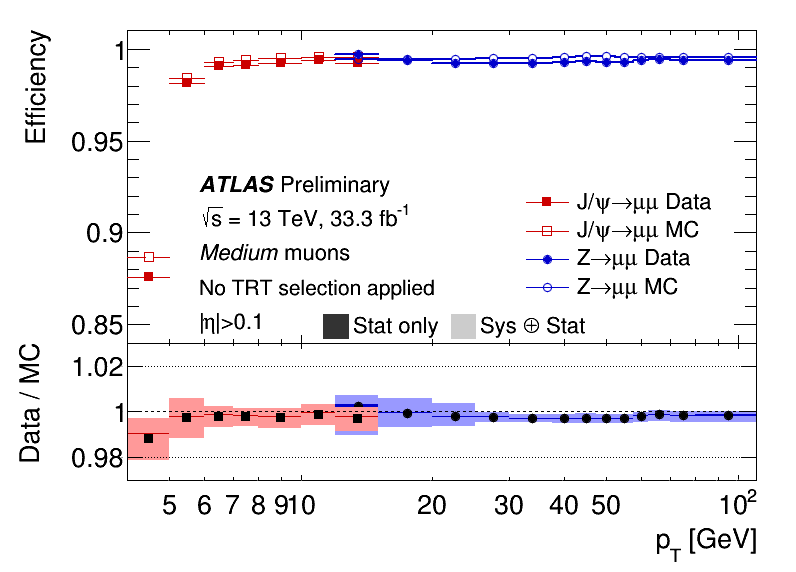
\includegraphics[width=0.7\linewidth]{figs/muon-eff}
	\caption{Muon reconstruction efficiencies for the Medium identification algorithm measured in $J/\psi \to \mu\mu$ and $Z \to \mu \mu$ events as a function of the muon momentum~\cite{Muon-ID-17}. 
		The prediction by the detector simulation is depicted as empty circles (squares), while the full circles (squares) indicate the observation in collision data. Only statistical errors are shown in the top panel. The bottom panel reports the efficiency scale factors. The darker error bands indicate the statistical uncertainty, while the lighter bands indicate the sum of the statistical and systematic uncertainties in quadrature.}
	\label{fig:muon-eff}
\end{figure}


Specifically for the searches described in this thesis, preselected muons are required to have $|\eta| < 2.7$ and $\pt > 5$~GeV. 
Muons must satisfy Medium identification requirements based on the number of hits in the different ID and MS subsystems, and the $q/p$ significance. The latter is defined as the absolute value of the difference between the ratio of the charge and momentum of the muons measured in the ID and MS divided by the sum in quadrature of the corresponding uncertainties~\cite{Aad_2016_muon}.

Events containing one or more muons that have a transverse impact parameter relative to the primary vertex $|d_0 | > 0.2$~mm 
or a longitudinal impact parameter relative to the primary vertex $|z_0 | > 1$~mm are rejected to suppress the cosmic-ray muon background.

\subsection{Signal Charged Leptons}
Signal light charged leptons, abbreviated as signal leptons, are preselected leptons surviving overlap removal and satisfying additional identification criteria. 
Signal electrons and muons must pass $\pt$-dependent isolation requirements, to reduce the contributions from semileptonic decays of hadrons and
jets misidentified as prompt leptons. 
The isolation requirements use calorimeter- and track-based information to obtain 95\% efficiency for charged leptons with 
$\pt = 25$~GeV in $Z \to e^+ e^-$ , $Z \to \mu^+ \mu^-$ events, rising to 99\% efficiency at $\pt = 60$~GeV. 
To improve the identification of closely spaced charged leptons (e.g. from boosted particle decays), 
contributions to the isolation from nearby electrons and muons passing all other signal lepton requirements are removed. 
To further suppress electrons and muons originating from secondary vertices, $|z_0 \sin \theta|$ is required to be less than 0.5~mm,
 and the $d_0$ normalized to its uncertainty is required to be small, with $|d_0 | /\sigma_{d_0} < 5(3)$ for electrons (muons). 
Signal electrons must also satisfy "medium" likelihood-based identification criteria, 
while signal taus must satisfy the "medium" Boosted Decision Trees-based identification criteria against jets.

\subsection{Taus}
The reconstruction of hadronically decaying tau candidates is seeded by jets.
Jets are constructed using the anti-$k_t$ algorithm with a distance parameter $R = 0.4$. 
Three-dimensional clusters of calorimeter cells called TopoClusters~\cite{Aad_2017-taus}, calibrated using a local hadronic
calibration~\cite{Barillari:1112035}, serve as inputs to the jet algorithm. 
Jets seeding tau candidates are  required to have $\pT > 10$~GeV and $|\eta| < 2.5$. 

The visible part of hadronically decaying tau leptons is conventionally referred to as \textit{taus} throughout the analyses described in this thesis.
Tau candidates in the transition region between the barrel and forward calorimeters, $1.37 < |\eta| < 1.52$, are vetoed.
A tau vertex is chosen as the candidate track vertex with the largest fraction of momentum from tracks
associated  with the jet in $\Delta R = \sqrt{(\delta\phi)^2 + (\delta\eta)^2}< 0.2$.
The tracks must pass requirements on the number of hits in the tracker and have $\pt > 1$~GeV. 
Additional requirements are placed on the shortest distance from the track to the tau vertex in the transverse plane, $|d_0| < $~mm, 
and the shortest distance in the longitudinal plane, $|\Delta_{ z_0} \sin\theta| < 1.5$~mm, where $\theta$ 
is the polar angle of the track and $z_0$ is the point of closest approach
along the longitudinal axis. 
Provided these requirements are passed the tracks are then associated to core ($0 < \Delta R < 0.2$) and isolation ($0.2 < \Delta R < 0.4$) 
regions around the tau candidate.

The direction ($\eta$, $\phi$) of the tau candidate is calculated using the vectorial sum of the TopoClusters within $\Delta R < 0.2$
of the seed jet barycenter, using the tau vertex as the origin. The mass of the tau candidate
is defined to be zero and consequently the transverse momentum, $\pT$, and the transverse energy, $E_T$ are
identical. The energy of the tau is obtained through dedicated calibration schemes which are described in depth in Ref.~\cite{ATLAS:2017mpa}.
Overall, the taus candidates are corrected to the visible hadronic energy scale using an $\eta$- and $\pt$-dependent calibration.

Tau candidates which are preselected for the SUSY analyses are required to have one or three associated tracks
(prongs), because taus predominantly decay to either one or three charged hadrons together with a neutrino and often additional neutral hadrons. 
The preselected taus are required to have $\pT > 20$~GeV and unit total charge of their constituent tracks. 

\begin{figure}
	\centering
	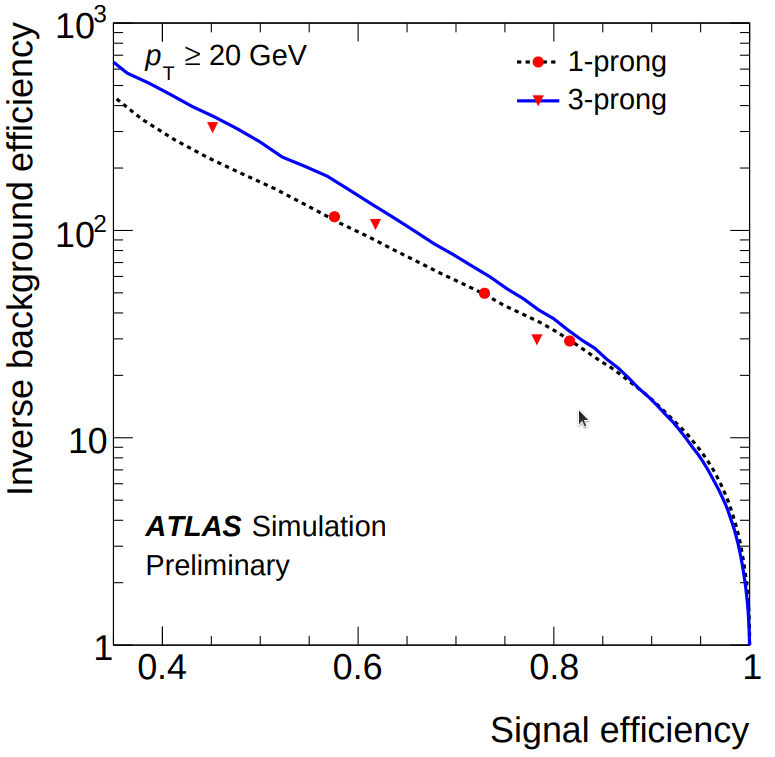
\includegraphics[width=0.6\linewidth]{figs/tau-eff}
	\caption{Inverse of the efficiency for mis-tagging QCD jets as a function of the identification efficiency for tau candidates. The two lines refer to 1-track and 3-track candidates. The Loose, Medium and Tight working points are shown on these lines. The working points do not stay exactly on the line because they implement variable cuts to achieve a reduced $\pt$-dependency of the efficiency. Adapted from Ref.~\cite{TheATLAScollaboration:2015lks}.}
	\label{fig:tau-eff}
\end{figure}
The tau identification is performed via a machine learning classification algorithm,
 which is designed to reject backgrounds from quark- and gluon-initiated jets~\cite{TheATLAScollaboration:2015lks}.
The identification uses Boosted Decision Trees (BDT) as classifier algorithm exploiting calorimetric and tracking information associated to the tau candidate. 
Three working points labelled ``loose", ``medium" and ``tight" are provided, and correspond to different tau identification efficiency values, with
the efficiency designed to be independent of $\pT$. 
The target efficiencies are 0.6, 0.55 and 0.45 for the generated 1-track loose, medium and tight working points, and 0.5, 0.4 and 0.3 for the corresponding
generated 3-track target efficiencies (Figure~\ref{fig:tau-eff}).
The input variables to the BDT are corrected such that the mean of their distribution for signal samples is constant as a function of pile-up. 
This ensures that the efficiency for each working point does not depend strongly on the pile-up conditions. 

Additionally, in order to suppress electrons misidentified as taus, taus are vetoed using transition radiation and calorimeter information.
An independent BDT algorithm is trained using discriminating track and cluster variables to optimize the tau identification against electrons, 
where ``loose", ``medium" and ``tight" working points are defined.

The performance of the identification and energy reconstruction algorithms is
evaluated with a data sample enriched in $Z \to \tau_\mu \tau_\text{had}$ events where one tau lepton decays to a muon and
the other decays hadronically, with associated neutrinos (Figure~\ref{fig:Ztaumu}). 
\begin{figure}
	\centering
	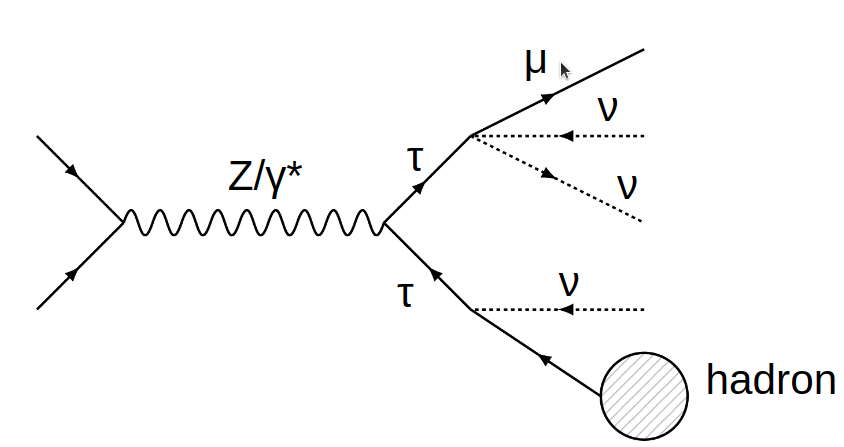
\includegraphics[width=0.6\linewidth]{figs/Ztaumu.png}
	\caption{Diagram of a $Z \to \tau_\mu \tau_\text{had}$ event used for tagging muons and probing the reconstruction and identification efficiency of the hadronically decaying tau lepton.}
	\label{fig:Ztaumu}
\end{figure}
The chosen tag-and-probe approach consists of selecting events triggered by the presence of a muon (tag) and containing a hadronically decaying
tau lepton candidate (probe) in the final state. The method studies the performance of the identification and energy reconstruction algorithms.
To select $Z \to \tau_\mu \tau_\text{had}$ events, a single-muon trigger with the threshold of $\pT > 20$~GeV is used.
 The offline reconstructed muon candidate must have $\pT > 22$~GeV and be geometrically matched to the online
muon. Events are required to have no additional electrons or muons and at least one hadronically decaying tau candidate with 1 or 3 tracks.
The muon and the tau candidate are required to have opposite-sign electric charges.

Figure~\ref{fig:tau-bdt-distr} shows the jet BDT score distribution for tau candidates which are probed in selected $Z \to \tau_\mu \tau_\text{had}$ events.
The efficiency for a given identification working point is calculated by taking the ratio of the extracted number of signal events before and after the identification criteria is applied. Finally, to account for the small differences between data and simulation, 
correction factors (also referred to as scale factors in ATLAS analyses), 
defined as the ratio of the efficiency in data to the efficiency in simulation for tau signal candidates to pass a certain level of identification, are derived.
These scale factors are then provided applied in the actual search analyses that involve taus in the final state.

\begin{figure}[htbp]
	\centering
	\begin{subfigure}[b]{0.48\textwidth}
		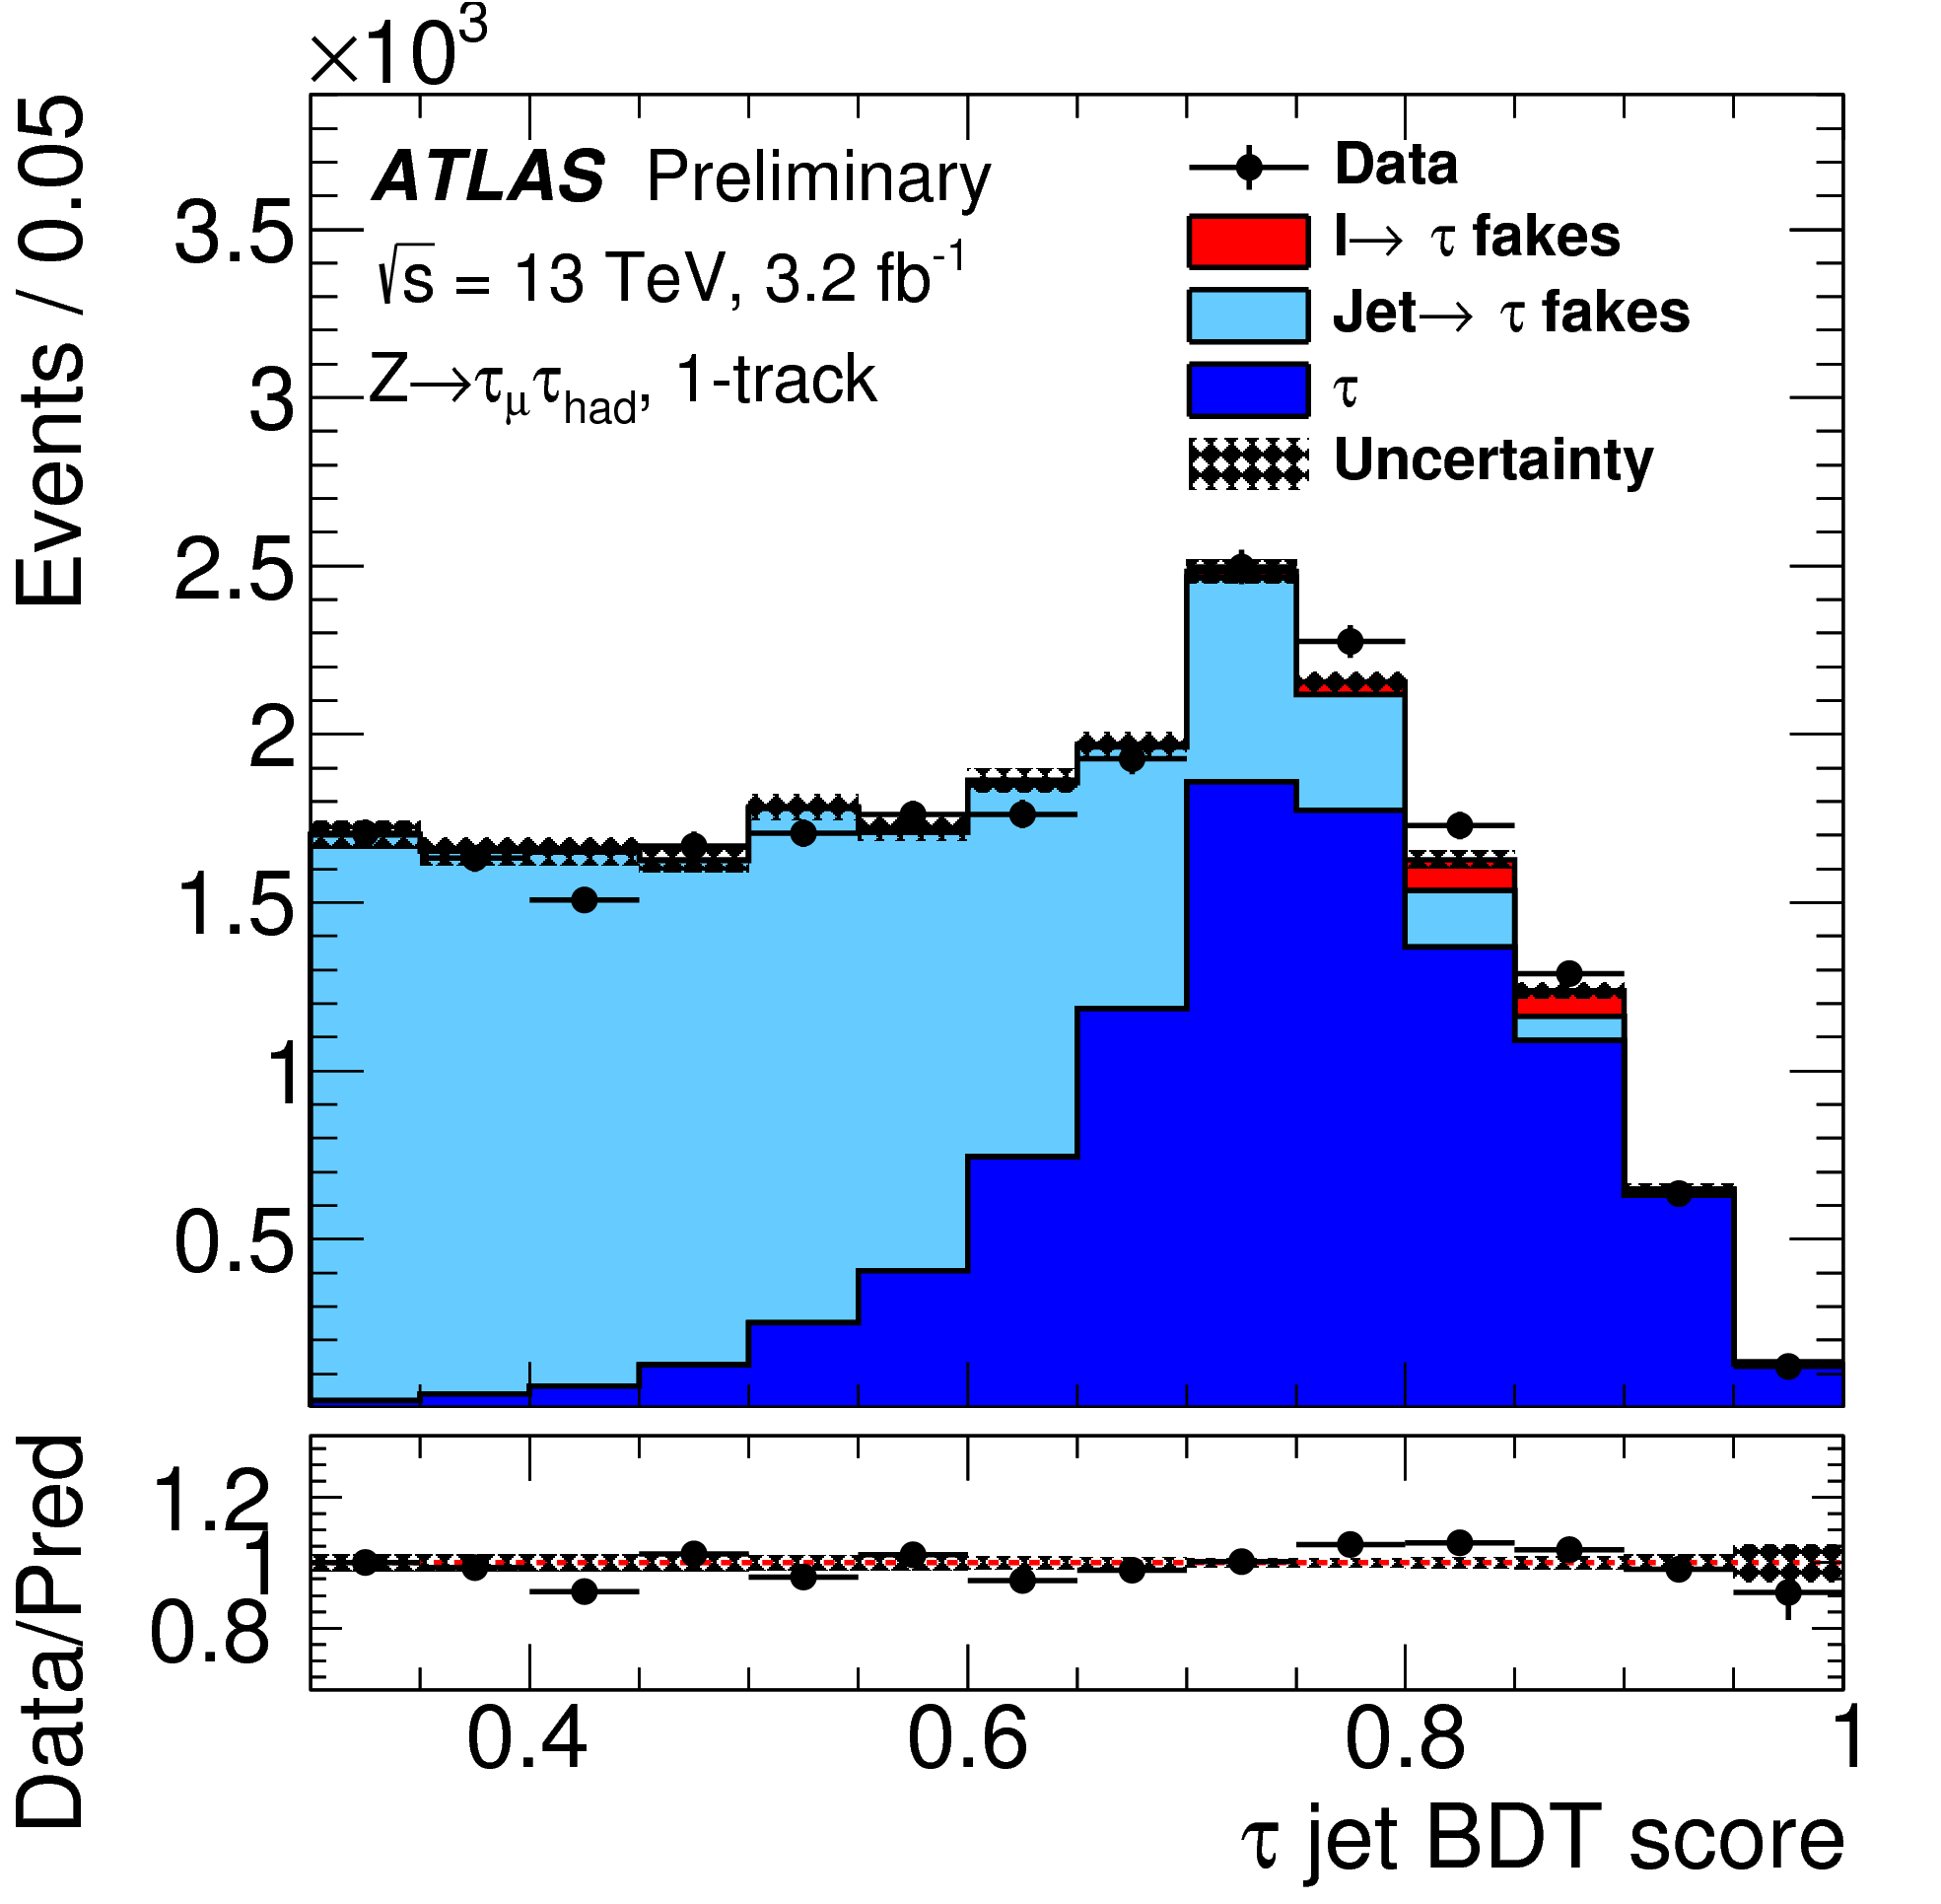
\includegraphics[width=\textwidth]{figs/tau-bdt-1.png}
		\caption{Wino W/Z NLSP}
		\label{fig:fig_01a}
	\end{subfigure}
	~ 
	\begin{subfigure}[b]{0.48\textwidth}
		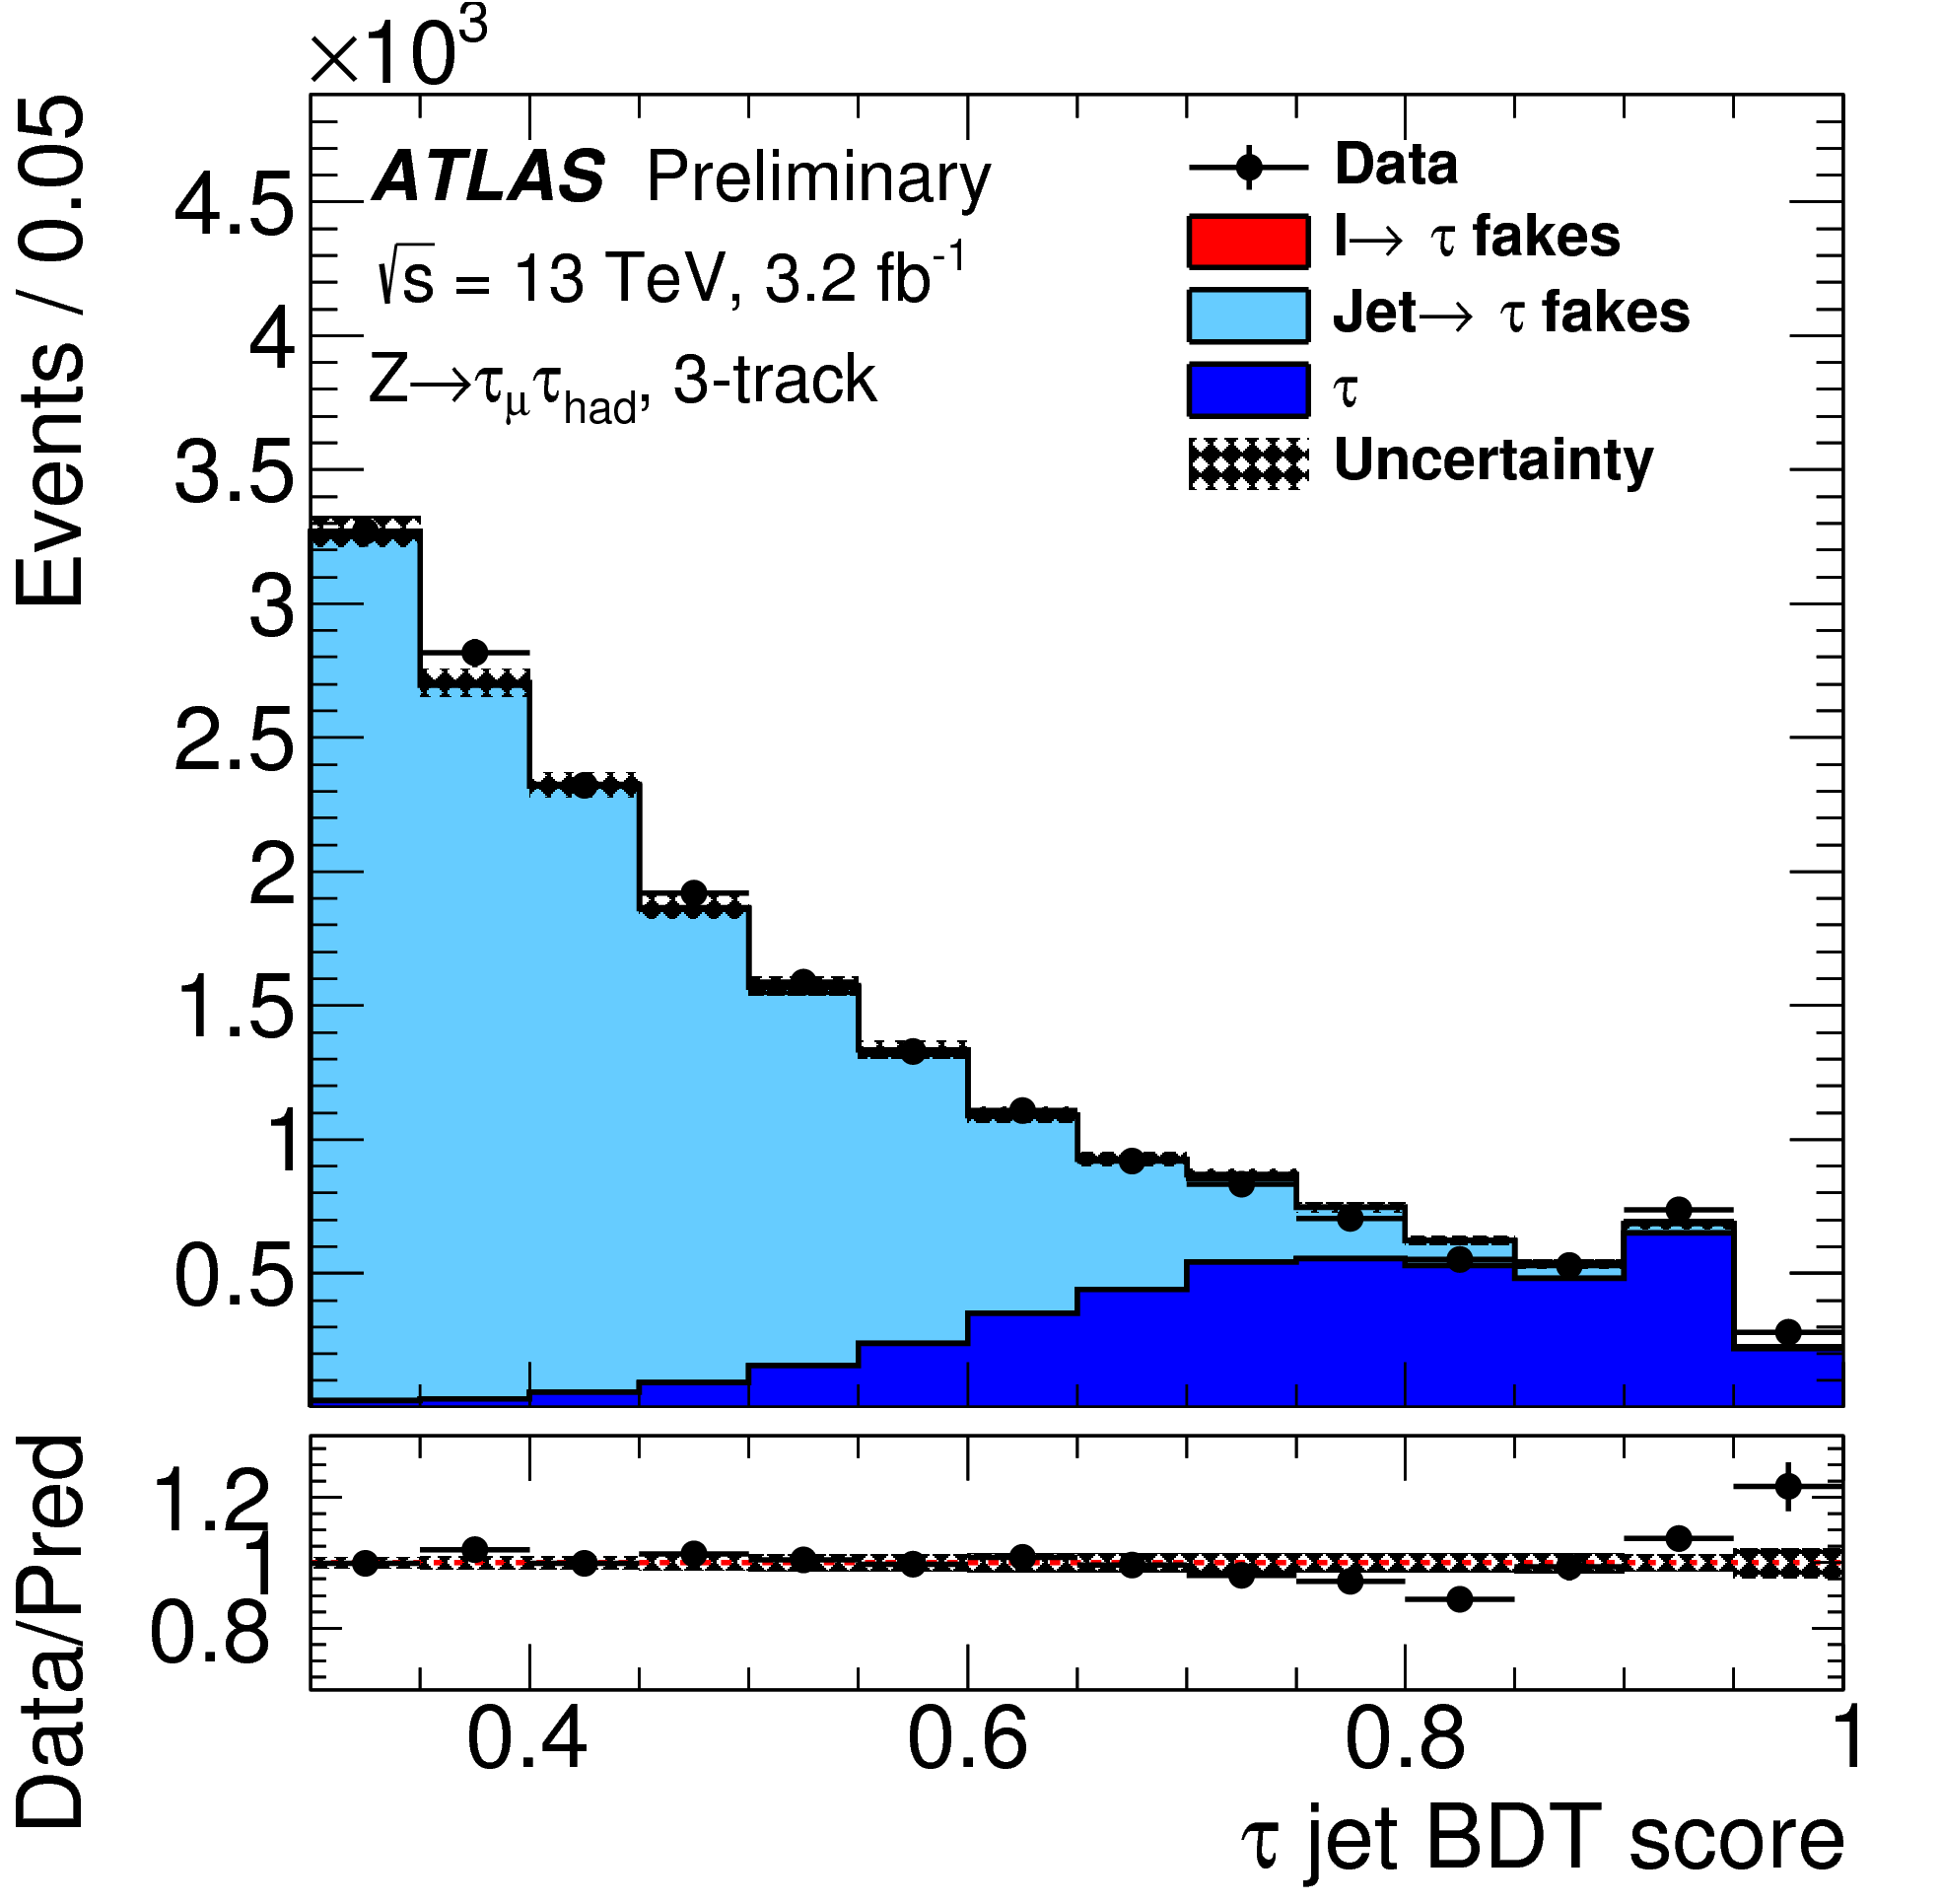
\includegraphics[width=\textwidth]{figs/tau-bdt-3.png}
		\caption{Wino W/h NLSP}
		\label{fig:fig_01b}
	\end{subfigure}
%
	\caption{The jet discriminant BDT output distribution for one track (left) and three track (right) hadronically decaying tau candidates. 
		The uncertainty band contains only the statistical uncertainty~\cite{ATLAS:2017mpa}.}\label{fig:tau-bdt-distr}
\end{figure}

\subsection{Jets}
Jets are reconstructed with the anti-$k_t$ algorithm with a radius parameter of $R = 0.4$~\cite{Cacciari-2008}. 
Three-dimensional calorimeter energy clusters are used as input to the jet reconstruction, and jets are calibrated
following Ref.~\cite{ATL-PHYS-PUB-2015-015}. 
Jets must be reconstructed in the barrel region $|\eta| < 2.8$ and have $\pt > 20$~GeV. 
To reduce pileup effects, jets with $\pt < 60$~GeV and $|\eta| < 2.4$ must satisfy additional criteria using the jet vertex tagging algorithm described
in Ref.~\cite{ATLAS:2015ull}. 
Events containing jets failing to satisfy the quality criteria described in Ref.~\cite{ATL-PHYS-PUB-2015-015} are rejected
to suppress events with large calorimeter noise or non-collision backgrounds.


\subsection{Missing Transverse Energy}
The missing transverse momentum, $E_\mathrm{T}^\mathrm{miss} = |\mathbf{E}_\mathrm{T}^\mathrm{miss}|$,
is the magnitude of the negative vector sum of the transverse momenta of all reconstructed and identified physics objects (electrons, photons, muons, taus and jets),
as well as an additional soft term,
\begin{equation*}
\mathbf{E}_\mathrm{T}^\mathrm{miss} = - \sum_{i} \mathbf{p}_{T,i} \quad \text{with} \quad i=\text{jets},\, \gamma,\, \mu,\, \tau,\, e,\, \text{soft terms} \, .
\end{equation*}
The soft term is constructed from the tracks matched to the primary vertex, but not associated with identified physics objects, which allows the soft term to be
nearly independent of pileup.


\section{Search for SUSY in Multileptonic Final States}

\subsection{Motivation}
Multileptonic final states consist a very attractive channel for the search for new physics at the LHC because the overwhelming hadronic background can be strongly suppressed. 
In RPV models, the lightest SUSY particle is unstable
and decays to SM particles, including charged leptons and neutrinos when violating L but not B. 
In RPC models, the LSP is stable and leptons can originate from unstable weakly interacting sparticles decaying into the LSP. 
Therefore, both the RPV and RPC SUSY scenarios can result in signatures with high lepton multiplicities and substantial missing transverse momentum.

Requiring a high multiplicity of isolated leptons (electrons and muons - including those originating from leptonic tau decays - and hadronically decaying taus), allows any new signature to be cleanly separated from the otherwise overwhelming hadron-rich background processes, typical of high-energy $pp$ collisions, even if its cross-section is small. 

More specifically, within this habilitation program, multiple searches for the production of charginos, neutralinos, sleptons and gluinos decaying to final states with at least four charged leptons are conducted. These searches exploit the complete $pp$ collision dataset delivered by the LHC at a center-of-mass energy of $\sqrt{s}=13$~TeV, and collected and reconstructed with the ATLAS detector. Particular emphasis is placed on the search for light higgsino particles. The exclusion of gluino and stop masses up to the TeV mass scale qualifies�now the light higgsinos to be discovered first at LHC, as motivated by naturalness (see Section~\ref{sec:Naturalness}). In General Gauge Mediated (GGM) SUSY models, the gravitino (supersymmetric particle of graviton) is nearly massless and is the LSP offering the possibility to study light higgsinos. Typical higgsino signal events are characterized by multiple charged leptons substantial missing transverse energy, which is a distinct signature used to identify higgsino events. 

The search itself is optimized using several signal models but is generally model-independent using loose requirements on effective mass or missing transverse energy. 
Results are presented in terms of the number of events from new physics processes with a four charged lepton signature, and in particular in terms of RPC or RPV
simplified models with decays of the LSP to charged leptons.

%The analysis was published in 2018~\cite{Aaboud:2018zeb} and presented at the ICHEP2018 and SUSY2018 conferences.

\subsection{Scenarios}

\subsubsection{R-Parity Violating Processes}
Simplified models of RPV scenarios are considered, where the LSP is a bino-like neutralino ($\tilde{\chi}^0_1$) and decays via an RPV interaction (see Section~\ref{sec:ChAndNeu}). The LSP decay is described by the $\frac{1}{2} \lambda_{ijk}L_i L_j \bar{E}_k$ lepton-number-violating superpotential term, where $L_i$ and $E_i$ indicate the lepton SU(2)-doublet superfield and singlet superfield, respectively. Lepton generations are referred to by the indices $i$, $j$ and $k$ while $\lambda_{ijk}$ corresponds to nine Yukawa couplings which allow the decay of the LSP to every possible combination of charged lepton pairs. In this search, two extremes of the $\lambda_{ijk}$ RPV couplings are considered: 
\begin{enumerate}
	\item $ L_1 L_2 \bar{E}_k\, (k=1,\,2)$ where only decays to electrons and muons are considered ($\lambda_{12k}\neq 0$), and 
	\item $ L_i L_3 \bar{E}_3\, (i=1,\,2)$ where only decays to taus and either electrons or muons are included ($\lambda_{i33}\neq 0$).
\end{enumerate}
In both scenarios, the remaining RPV couplings are considered to be zero. Figure~\ref{fig:RPV-BR} shows the branching ratios for the LSP decay in the $ L_1 L_2 \bar{E}_k$ and $ L_i L_i \bar{E}_3$ scenarios. The search of Yukawa couplings not included in the searched scenarios. For example, the $\lambda_{123}$ RPV couplings is expected to lie in the sensitivity achieved between $ L_1 L_2 \bar{E}_k$ and $ L_i L_i \bar{E}_3$.
\begin{figure}[htbp]
	\centering
	\begin{subfigure}[b]{0.48\textwidth}
		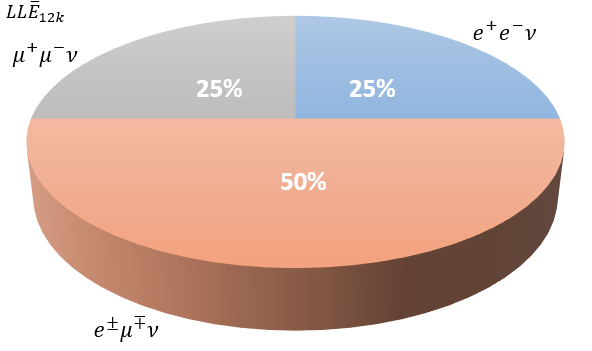
\includegraphics[width=\textwidth]{figs/LLE12k.png}
		\caption{$ L_1 L_2 \bar{E}_k\, (k=1,\,2)$ decays involving electrons, muons and neutrinos.}
	\end{subfigure}
	~ 
	\begin{subfigure}[b]{0.48\textwidth}
		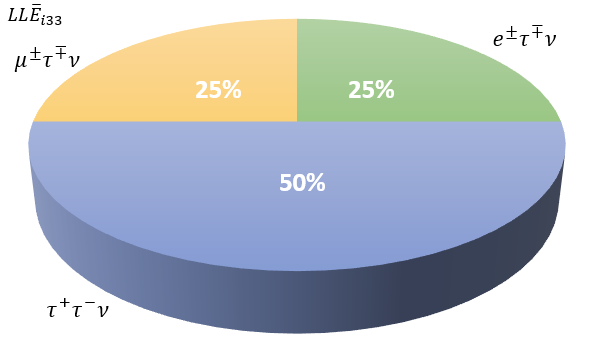
\includegraphics[width=\textwidth]{figs/LLEi33.png}
		\caption{$ L_i L_3 \bar{E}_3\, (i=1,\,2)$ decays involving at least two taus and any other lepton.}
	\end{subfigure}
	\caption{Decay modes and branching ratios for the $\tilde{\chi}^0_1$ LSP in the RPV models, where $\nu$ denotes neutrinos or
		antineutrinos of any lepton generation.}\label{fig:RPV-BR}
\end{figure}


Three different RPV scenarios are searched in this thesis for the next-to-lightest-supersymmetric particle (NLSP) in the $ L_1 L_2 \bar{E}_k$ ($\lambda_{12k}$) and $ L_i L_3 \bar{E}_3$ ($\lambda_{i33}$): 
\begin{enumerate}
 \item Wino NLSP, where mass-degenerate wino-like charginos and neutralinos are produced in association;
 \item Slepton/sneutrino NLSP, where mass-degenerate left-handed sleptons and sneutrinos of all three generations are produced in association; and 
 \item Gluino NLSP, where the produced gluinos decay to the LSP while emitting a quark-antiquark pair each.
\end{enumerate}

These scenarios, as diagrammatically shown in Figure~\ref{fig:RPV_models},  result typically in signatures with high lepton multiplicities and substantially high values of the the effective mass observable, $m_\text{eff}$.
These features of the final state can be used to select signal events while suppressing the  SM background drastically.

\begin{figure}[htbp]
 \centering
 \begin{subfigure}[b]{0.35\textwidth}
  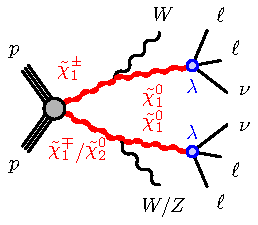
\includegraphics[width=\textwidth]{figs/fig_01a.pdf}
  \caption{Wino W/Z NLSP}
  \label{fig:fig_01a}
 \end{subfigure}
 ~ 
 \begin{subfigure}[b]{0.35\textwidth}
  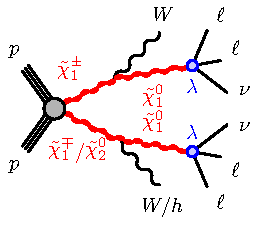
\includegraphics[width=\textwidth]{figs/fig_01b.pdf}
  \caption{Wino W/h NLSP}
  \label{fig:fig_01b}
 \end{subfigure}
 \\
 \begin{subfigure}[b]{0.35\textwidth}
  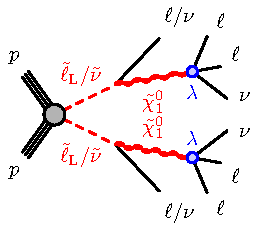
\includegraphics[width=\textwidth]{figs/fig_01c.pdf}
  \caption{Slepton/sneutrino NLSP}
  \label{fig:fig_01c}
 \end{subfigure}
 %
 \begin{subfigure}[b]{0.35\textwidth}
  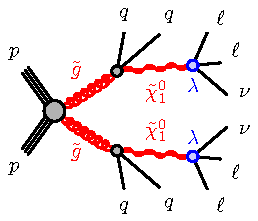
\includegraphics[width=\textwidth]{figs/fig_01d.pdf}
  \caption{Gluino NLSP}
  \label{fig:fig_01d}
 \end{subfigure}
%
 \caption{Diagrams of the processes in the SUSY RPV models considered in the analysis: 
 	\ref{fig:fig_01a} and \ref{fig:fig_01b} a wino, \ref{fig:fig_01c} a slepton and \ref{fig:fig_01d} gluino NLSP, followed by the RPV decay of 
 	the $\tilde{\chi}^0_1$ LSP with a $\mathrm{BR(\tilde{\chi}^0_1 \to \ell \ell \nu)}$ of 100\%.}\label{fig:RPV_models}
\end{figure}

\subsubsection{R-Parity Conserving Processes}
This analysis is also optimized to search RPC scenarios with light $\tilde{\chi}^0_1 \, \tilde{\chi}^0_2 \, \tilde{\chi}^\pm_1$ higgsino triplet states in the context of GGM, which predicts the gravitino ($\tilde{G}$, the fermionic superpartner of the graviton) nearly massless giving the opportunity to study light higgsinos (shown in Figure~\ref{fig:hino}). Light higgsinos are well motivated by naturalness~\cite{BARBIERI198863, deCarlos:1993rbr}, as discussed in Section~\ref{sec:Naturalness}.
\begin{figure}[htbp]
\centering
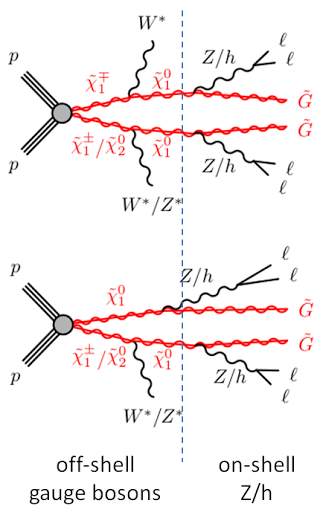
\includegraphics[width=0.4\linewidth]{figs/ggm}
\caption{Diagrams of the processes in the GGM higgsino models considered in the analysis.}
\label{fig:hino}
\end{figure}

Typically, the members of the higgsino triplet are close in mass its decays result in low-momentum decay products that are difficult to reconstruct efficiently. However, the decays of the higgsinos themselves to the LSP gravitino, $\tilde{G}$, would lead to on-shell Z/h, and the decay products can be therefore efficiently reconstructed, as illustrated in Figure~\ref{fig:ggm}.
\begin{figure}[htbp]
 \centering
 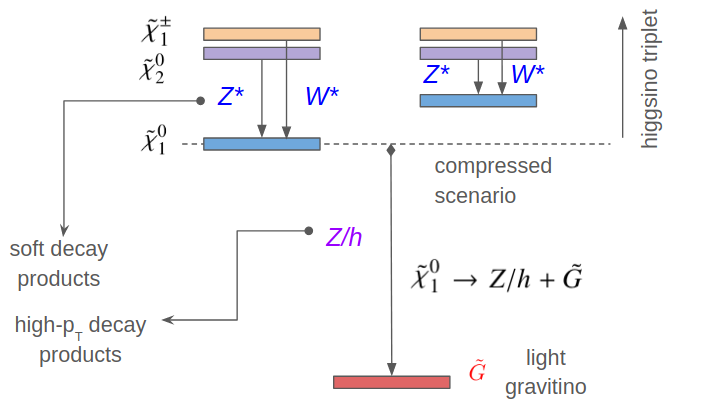
\includegraphics[width=0.7\linewidth]{figs/hino}
 \caption{Chart illustrating the decay chain of the higgsino triplet $\tilde{\chi}^0_1$, $\tilde{\chi}^0_2$, $\tilde{\chi}^\pm_1$ to a nearly massless gravitino, $\tilde{G}$, LSP. The decays of the higgsinos to the LSP would lead to on-shell Z/h, and the decay products can be thus reconstructed. }
 \label{fig:ggm}
\end{figure}
In this search, simplified RPC models inspired by GGM are considered, where the only SUSY particles within reach of the LHC are an almost mass-degenerate higgsino triplet $\tilde{\chi}^0_1\, \tilde{\chi}^0_2\, \tilde{\chi}^\pm_1$ and a massless $\tilde{G}$. Finally, the $ \tilde{\chi}^0_1 \to Z \tilde{G}$ branching ratio is a free parameter of the GGM higgsino scenarios, and so offers an opportunity to study four-lepton signatures with one or more Z-boson candidates.

\subsection{Methodology}

\subsubsection{Event categorization strategy}
Events are selected using single-lepton or dilepton triggers, where the trigger efficiencies are in the plateau
region above the offline $p_\mathrm{T}$ thresholds. The latter are typically a bit higher than the online ones. Dilepton triggers are used only when the leptons in the event fail $p_\mathrm{T}$-threshold requirements for the single-lepton triggers.

Events with four or more signal leptons ($\ell =e,\, \mu$ and hadronically decaying $\tau_\mathrm{had-vis}$) are selected and are classified according to the number of light signal leptons (L = e, $\mu$) and signal taus (T): at least four light leptons and exactly zero taus 4L0T, exactly three light leptons and at least one tau 3L1T, or exactly two light leptons and at least two taus 2L2T .

Events are further classified according to whether they are consistent with a leptonic Z boson decay or not. The Z-boson requirement selects events where any same-flavor LL pair combination with opposite electric charge (SFOS)  has an invariant mass close to the Z-boson mass, in the range $81.2-101.2$~GeV. A second Z boson candidate may be identified if a second SFOS LL pair is present and satisfies $61.2 < m(LL) < 101.2$~GeV.
To suppress radiative Z boson decays into four leptons (where a photon radiated from a $Z \to \ell \ell$ decay converts to a second SFOS lepton pair) the Z veto also considers combinations of any SFOS LL pair with an additional lepton (SFOS+L), or with a second SFOS LL pair (SFOS+SFOS), and rejects events where either the SFOS+L or SFOS+SFOS invariant mass lies in the range $81.2-101.2$~GeV.


In order to separate the SM background from SUSY signal, the $E_\mathrm{T}^\mathrm{miss}$ and the effective mass of the event, $m_\mathrm{eff}$, are both used. More precisely, the $m_\mathrm{eff}$ is constructed as the scalar sum of the $E_\mathrm{T}^\mathrm{miss}$, the $p_\mathrm{T}$ of signal leptons and the $p_\mathrm{T}$ of all jets above 40 GeV (in order to suppress jets stemming  from pileup events and the underlying event).

The event selection strategy is depicted in Figure~\ref{fig:event-selection}.
GGM Higgsino event selection targets events with at least four light leptons, relatively low $m_\mathrm{eff}$  and low or high reconstructed $E_\mathrm{T}^\mathrm{miss}$ in the event. The selection targeting RPV multilepton SUSY scenarios is optimized according to the number of additional hadronically decaying tau leptons and the reconstructed $m_\mathrm{eff}$ that characterizes the event.
\begin{figure}
	\centering
	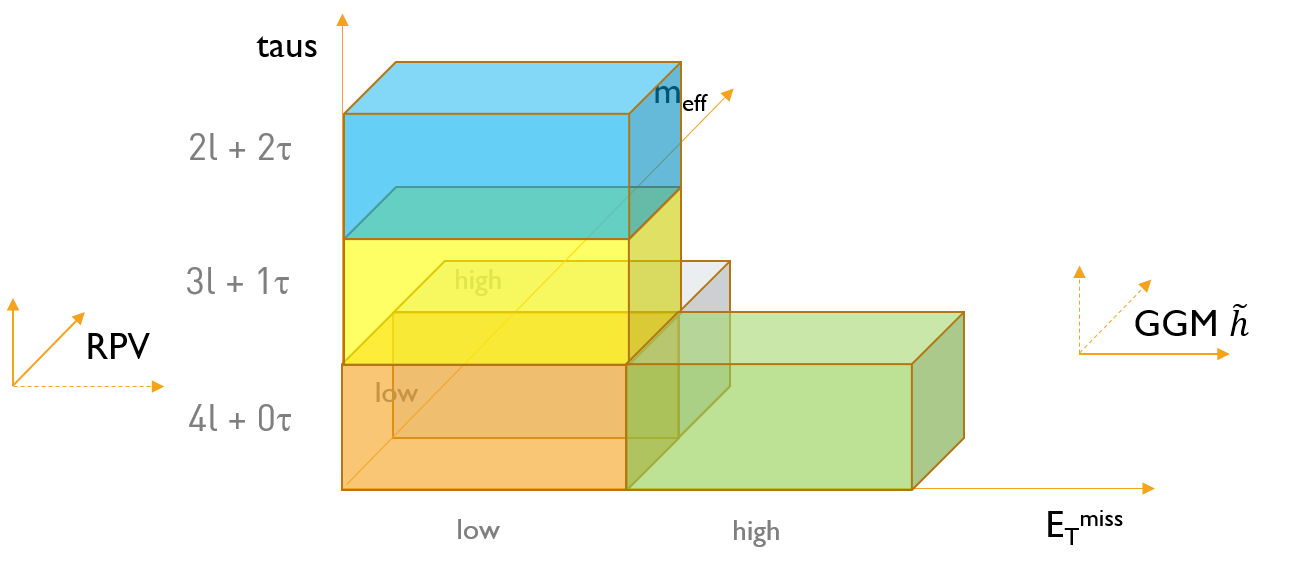
\includegraphics[width=0.95\linewidth]{figs/event-selection}
	\caption{Illustration of the event selection strategy in terms of light lepton multiplicity and the number of hadronically decaying tau leptons associated to the final state event, the reconstructed transverse missing energy,  $E_\mathrm{T}^\mathrm{miss}$, and the effective mass, $m_\mathrm{eff}$.}
	\label{fig:event-selection}
\end{figure}

\subsubsection{Trigger Strategy}
The data used for the four-lepton search are selected with triggers that require the presence of isolated electrons and muons. 
Events are selected using single-lepton or dilepton triggers, 
where the trigger efficiencies are in the plateau region above the offline $\pt$ thresholds indicated in Table~\ref{tab:triggers}.
Dilepton triggers are used only when the leptons in the event fail the $\pt$-threshold requirements for the single-lepton triggers.
\begin{table}[h]
	\begin{center}
		\small{
			\begin{tabular}{ l ll }
				\hline
				Trigger                            & \multicolumn{2}{l}{Offline $\pt$ threshold [GeV] } \\
				& 2015              & 2016                              \\ \hline
				Single isolated $e$                & 25                & 27                                \\
				Single non-isolated $e$            & 61                & 61                                \\
				Single isolated $\mu$              & 21                & 25 or 27                          \\
				Single non-isolated $\mu$          & 41                & 41 or 51                          \\ \hline
				Double $e$                         & 13, 13            & 18, 18                            \\ \hline
				Double $\mu$ { \textit (symmetric)}     & --                & 11, 11 or 15, 15                  \\
				~~~~~~~~~~~~~~~~{\textit(asymmetric)} & 19, 9             & 21, 9 or 23, 9                    \\ \hline
				Combined $e\mu$                    & 8($e$), 25($\mu$) & 8($e$), 25($\mu$)                 \\ \hline
			\end{tabular} 
		}       
		\caption{The triggers used in the analysis of 2015 and 2016 data. 
			The offline $\pt$ thresholds are required only for reconstructed charged leptons which match to the trigger signatures. 
			Trigger thresholds for data recorded in 2016 are higher than in 2015 due to the increase in beam luminosity, and ``or'' denotes a move to a higher-threshold trigger during data-taking.
			\label{tab:triggers} }
	\end{center}
\end{table}

Leptons triggering the event are required to pass signal lepton requirements, be within $\Delta R < 0.1$ from the relevant trigger object and pass offline $\pt$ thresholds that ensure the lepton is sufficiently far away from the turn-on of the trigger efficiency.
For electron triggers, the offline $\pt$ threshold is $1$~GeV higher than the trigger threshold.
For single muon triggers, the offline $\pt$ threshold is $1.05\times$ the trigger threshold, and $+1,\,2$~GeV for dimuon triggers.


The triggers are exclusively applied to different phase-space regions, typically defined by the transverse momentum of the analysis' lepton candidates.
An example of a trigger combination is diagrammatically shown in Figure~\ref{fig:electrons-2017-b4-b8}. 
The offline signal lepton candidates showing up in this trigger scheme must be fulfill the trigger matching requirements and a pass a certain offline $p_T$ threshold based on the trigger efficiency turn-on curve, in order to apply the appropriate trigger efficiency correction to the simulated event.
\begin{figure}
	\centering
	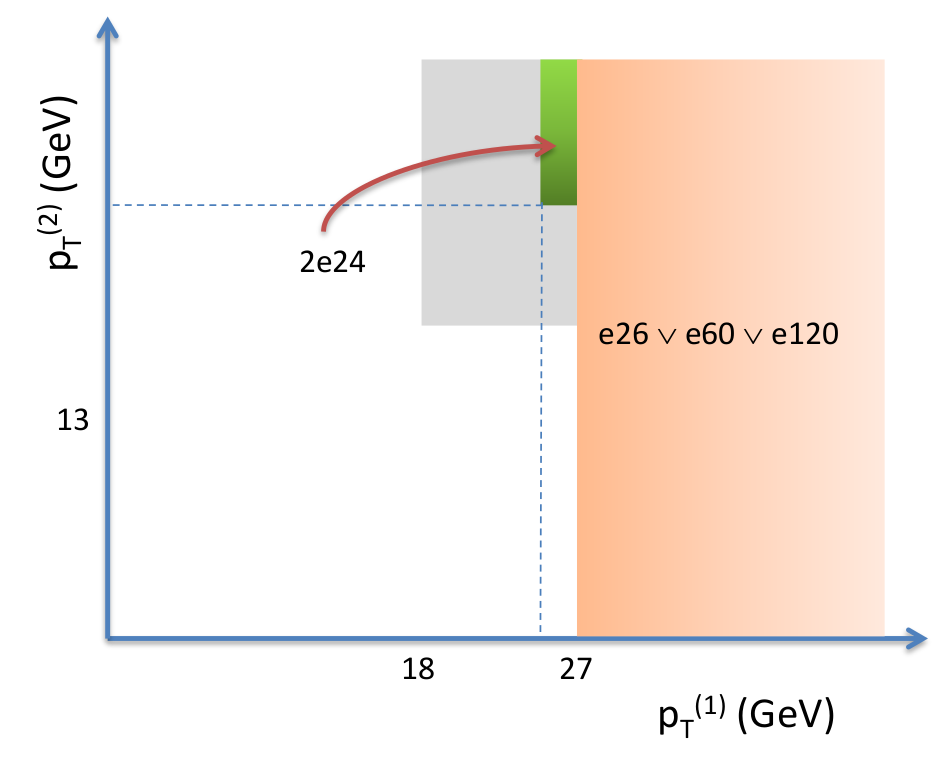
\includegraphics[width=0.6\linewidth]{figs/electrons-2017-B4-B8}
	\caption{Example of combining single- and double-lepton triggers for data collected in a sub-period of year 2017. 
	The horizontal axis represents the reconstructed transverse momentum of the leading signal lepton in the final state. 
	The vertical axis corresponds to the possible sub-leading signal lepton in the event that may cause the di-lepton trigger to fire the event.
	The kinematic area marked with orange color is covered by a logical OR between single trigger with various $\pt$ thresholds, \texttt{e26}, \texttt{e60} and
	\texttt{e120} (values expressed in GeV), each having different online identification and isolation requirements.
	The green area represents multilepton events selected by a dielectron trigger with a symmetric  $\pt$ threshold at 24~GeV. 
	The gray area represents the kinematic phase space covered by a trigger with lower $\pt$ thresholds (\texttt{2e17}) in
	precedent  data LHC runs with lower instantaneous luminosity. As the instantaneous luminosity increases in time, the trigger thresholds increase dynamically in order to cope with the highest collision rates.}
	\label{fig:electrons-2017-b4-b8}
\end{figure}


Since multiple leptons may trigger the event, the triggering scheme is simplified according to the following priority:
\begin{enumerate} \itemsep0pt
	\item If a single or di-electron trigger fires, then apply the $e/\gamma$-related trigger scale factors and associated trigger efficiency uncertainties;
	\item Else, if a single or di-muon trigger fires, then apply the muon-related trigger scale factors and associated trigger efficiency uncertainties;
	\item Else, if a combined electron+muon trigger fires, then apply product of the $e/\gamma$- and muon-related trigger scale factors and corresponding uncertainties to the respective trigger signature  of the trigger item;
	\item The event fails the trigger requirements and is rejected from the analysis.
\end{enumerate}

Trigger efficiencies are measured in data and simulation, and scale factors are applied to MC simulated events to correct the MC trigger simulation to that in data. The applied scale factors are typically parameterized in the $\pt$ and $\eta$ of the reconstructed electron and muon candidates that match to the trigger signature used to select the event. The triggering efficiency for events with four, three and two electrons/muons in signal SUSY scenarios is typically $>$99\%, 96\% and 90\%, respectively. 




\subsubsection{Signal regions}
Two signal regions (SR) are defined with 4L0T and a Z-boson veto: a general, model-independent signal region
(SR0A) with $m_\mathrm{eff}>600$~GeV, and a tighter signal region (SR0B) with $m_\mathrm{eff}>1.1$~TeV, optimized for the RPV $LL\bar{E}_{12k}$ scenarios. 
%
Two further SRs are defined with 4L0T, a first and second Z requirement and different selections on  $E_\mathrm{T}^\mathrm{miss}$: a loose signal region (SR0C) with $E_\mathrm{T}^\mathrm{miss}>40$~GeV, and
a tighter signal region (SR0D) with $E_\mathrm{T}^\mathrm{miss}>100$~GeV, optimized for the low-mass and high-mass higgsino
GGM scenarios, respectively. Finally, two SRs are optimized for the tau-rich RPV $LL\bar{E}_{i33}$ scenarios: one
with 3L1T where the tau has $p_\mathrm{T} > 30$~GeV, a Z veto and $m_\mathrm{eff}>700$~GeV (SR1), and a second with 2L2T
where the taus have $p_\mathrm{T} > 30$~GeV, a Z veto and $m_\mathrm{eff}>650$~GeV (SR2).
%
All signal regions deployed in the search are diagrammatically shown by Figure~\ref{fig:categ}.
\begin{figure}
 \centering
 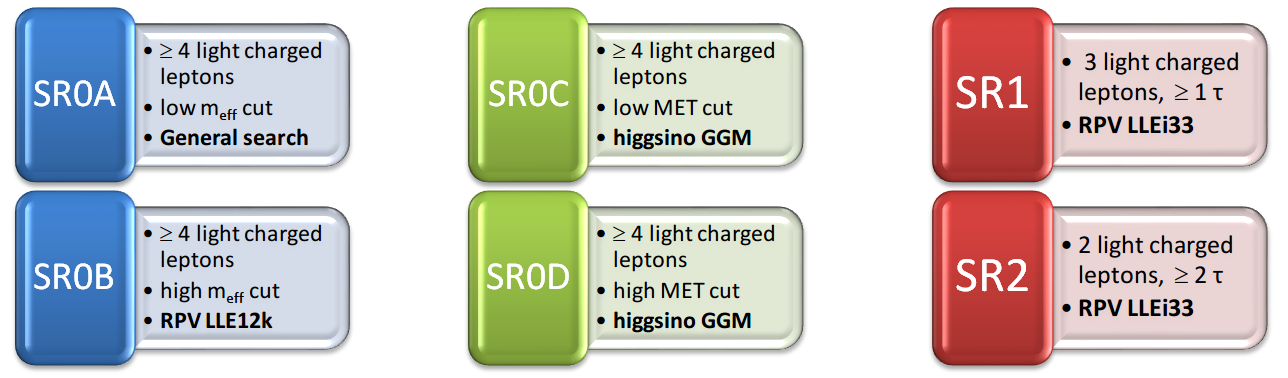
\includegraphics[width=0.95\linewidth]{figs/categ}
 \caption{Signal regions targeting RPV and RPC SUSY signal events. SR0A, SR0B, SR1 and SR2 target SUSY events in RPV scenarios, while SR0C and SR0D are designed to be sensitive to GGM higgsino SUSY events.}
 \label{fig:categ}
\end{figure}

\subsubsection{Background processes}
In general, the search of SUSY processes with four leptons in the final state suffers less by background processes as the known SM four-lepton processes are few with very 
low production cross-section. Nevertheless, several SM processes can result in signatures resembling SUSY signals with four reconstructed charged
leptons, including both the ``real" and ``fake" lepton contributions.
In this search, a real charged lepton is defined to be a prompt (i.e. not stemming from a secondary particle decay) 
and genuinely isolated lepton (i.e. no track activity in the nearby phase-space of $\Delta R < 0.2$).
A fake charged lepton is defined to be a non-prompt or non-isolated lepton that could originate from any of the following:
\begin{itemize}
	\item semileptonic decays of b- and c-hadrons, 
	\item in-flight decays of light mesons,
	\item misidentification of particles within light-flavor,
	\item gluon-initiated jets, or
	\item photon conversions.
\end{itemize}


The main background processes of this search are thus classified into two categories (Figure~\ref{fig:bkg}):
\begin{enumerate}
 \item  irreducible background consisting of hard-scattering processes giving rise to events with four or more real leptons (e.g. $ZZ$ and $t\bar{t}Z$); and  
 \item reducible background consisting of processes leading to events with at least one fake lepton (e.g. $t\bar{t}$, Z+jets and WW).
\end{enumerate}
Backgrounds with three or more fake leptons (e.g. W+jets) are found to have a negligible contribution to this analysis. 
The systematic uncertainty on the reducible background is increased in order to cover any effect from such type of background sources.

The irreducible backgrounds are estimated from Monte Carlo (MC) simulation, while the reducible backgrounds are derived from data with the so-called \textit{fake-factor} method, which is subject of the next section.

\begin{figure}[h!]
	\centering
	\begin{subfigure}[b]{0.3\textwidth}
		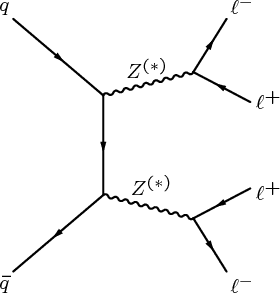
\includegraphics[width=\textwidth]{figs/ZZ.png}
		\caption{ZZ decay to leptons}
	\end{subfigure}
	~ 
	\begin{subfigure}[b]{0.4\textwidth}
		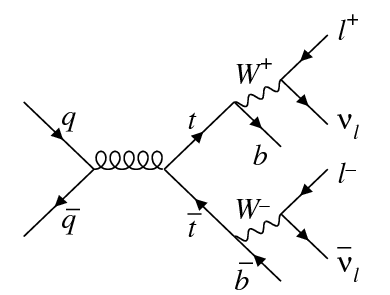
\includegraphics[width=\textwidth]{figs/ttbar.png}
		\caption{$t\bar{t}$ decay to leptons}
	\end{subfigure}
	\caption{Example processes for irreducible (left) and reducible (right) backgrounds of the four-lepton SUSY search.}\label{fig:bkg}
\end{figure}

\subsubsection{Reducible background estimate}

As mention before, the definition of reducible background in this analysis is any signal-like event that includes at least one lepton that does not arise from the prompt decay of a $W^\pm$ boson, Z boson, top quark or a Higgs boson, or, of course, a SUSY particle.
The dominant reducible backgrounds in the signal regions are $t\bar{t}$ and Z+jets processes.

The technique for estimating the reducible background relies on the introduction of control regions for each signal region that have identical kinematic selection criteria, but inverted selection criteria on one or two of the reconstructed leptons:
\begin{description}
	\item[SR:] Four or more signal leptons, any number of loose leptons,
	\item[CR1:] Exactly three signal leptons, at least one loose lepton,
	\item[CR2:] Exactly two signal leptons, at least two loose leptons,
\end{description}
where the reducible background composition is calculated for each region separately.
Specifically, ``loose" leptons are leptons surviving the geometrical overlap removal with respect to other reconstructed particles in the event, but do not satisfy signal lepton criteria. 

Subsequently, in the fake-factor method, the number of reducible background events in a given region is estimated from data using probabilities for a fake charged lepton ($e$, $\mu$ and hadronically decaying tau leptons) to pass or fail the signal lepton selection. 
The ratio 
\begin{equation}
F = \frac{f}{  \bar{f} }
\end{equation} 
for fake leptons is the "fake factor", where f ($\bar{f}$) is the probability that a fake lepton is misidentified as a signal ("loose") lepton. 
The probabilities used in the fake-factor calculations are based on simulation and corrected to data where possible.

%For this fake-factor evaluation, a very loose selection on the identification BDT is also applied to the preselected taus, since candidates with very low BDT scores are typically gluon-induced jets and jets arising from pileup, which is not the case for the signal tau candidates.

In practice, $F$ is seen to vary with physics process, the source of the fake lepton (heavy/light flavour decay, conversion), lepton flavour, $\pt$, and $\eta$, and possibly other variables. 
The fake factors for each lepton source $i$ and MC process $j$ are calculated from MC events with 1--2 leptons, and the overall fake factor for region $XR$ is weighted according to the expected fractional contribution $f$ from each SM process and lepton source

\begin{equation}
F_{XR}^{\ell}(\pt,\eta)=\sum_{i, j} \left(  f_{XR}^{ij}(\pt) \cdot sf^{i}(\pt) \cdot F^{ij}(\pt,\eta) \right)
\label{eq:FakeFactorDef_weighted}
\end{equation}
where, the fake factor for each fake lepton source is corrected to data using $sf$ 

Once $F$ has been calculated appropriately for the given signal region, 
the control region events are weighted according to the loose leptons that they contain to estimate the total number of events in the signal region. In general,

\begin{align}\label{eq:FakeFactorMethod} 
N_{\mathrm{SR}}^{\mathrm{SM}} & =  N_{\mathrm{SR}}^{\textrm{SM,irreducible}} \\
& + \left( N_{\mathrm{CR1}}^{\mathrm{data}} - N_{\mathrm{CR1}}^{\textrm{SM,irreducible}} \right) \cdot F \\
& - \left( N_{\mathrm{CR2}}^{\mathrm{data}} - N_{\mathrm{CR2}}^{\textrm{SM,irreducible}} \right) \cdot F_1 F_2 \\
& + \left( N_{\mathrm{CR3}}^{\mathrm{data}} - N_{\mathrm{CR3}}^{\textrm{SM,irreducible}} \right) \cdot F_1 F_2 F_3 \\
& - \left( N_{\mathrm{CR4}}^{\mathrm{data}} - N_{\mathrm{CR4}}^{\textrm{SM,irreducible}} \right) \cdot F_1 F_2 F_3 F_4 ,
\end{align}
where, 
\begin{itemize}
	\item $N_{\mathrm{CRX}}^{\mathrm{data}}$ represents the control region events in data with $X$ loose leptons, 
	\item $N_{\mathrm{CRX}}^{\textrm{SM,irreducible}}$ represents the estimated number of irreducible events in the control region (e.g. from $t\bar{t}Z$ and $ZZ$ processes), and
	\item  $F$ and $F_i$ represent the fake factor from the loose lepton(s) in the event. 
\end{itemize}
Furthermore, the third term removes the double counting of events with two fake leptons in the second term.
The fourth and fifth terms in Equation~\eqref{eq:FakeFactorMethod} are not used in the analysis, as the contribution from processes with three and four fake leptons in MC simulation is negligible.
However, a systematic uncertainty is included to account for neglected higher order terms.
In the analysis, the control regions for LLLL events are indicated as CR1\_LLLl and CR2\_LLll, where L and l refer to signal and loose light leptons, respectively.
Similarly, ``4L'' indicates a signal region selection with four light signal leptons.

The reducible background prediction is thereby extracted by applying fake factors to control regions (CR) in data. The CR definition only differs from that of the associated SR in the quality of the required leptons. The fake factors are applied on an event-by-event basis rather than as an average.
% here exactly one (CR1) or two (CR2) of the four leptons must be identified as a loose lepton, as shown in Table 5. 
%In 3L1T events, the contribution from events with two fake light leptons is negligible, as is the contribution from one and two fake light leptons in 2L2T events.
Finally, the predictions for irreducible and reducible backgrounds are tested in validation regions (VR).

In practice, fake electrons, muons and taus arise from following main sources:
\begin{description}
	\item[Heavy flavour (HF) leptons] arise from the semileptonic decays of hadrons that contain $b$ or $c$ quarks.
	These are the dominant source of fake leptons in $t\bar{t}$ events.
	\item[Light flavour (LF) electrons and muons] arise from other hadronic processes.
	For electrons, this usually involves a single hadron being misidentified as an electron.
	Various processes can produce LF muons, including in-flight pion decays.
	\item[Conversion (CO) electrons] arise from interactions of photons with material in the ATLAS detector.
	This process is negligible for muons.
	\item[Quark Jet (QJ) taus] arise from the misidentification of a hadronic jet as a hadronic tau. The jet is initiated by a quark/hadron and the presence of charged particles results in a higher fake rate than from gluon-initiated jets.
	\item[Gluon Jet (GJ) taus] again arise from the misidentification of a hadronic jet as a hadronic tau. However, the gluon-initiated jet results in few charged particles and a in a lower fake rate than from quark-initiated jets.
	\item[Unknown (UN) sources] are the small fraction of fake leptons that cannot be classified as any of the above sources. Such cases originate predominantly from secondary interactions other than the hard interaction of the collision event, such as pile-up or underlying events.
\end{description}
The fake factors are calculated for each MC process ($t\bar{t}$, $Z+$jets, ...) and lepton source are calculated from MC events with 1--2 leptons. 
Figures~\ref{fig:FF-LL} and \ref{fig:FF-TAU} show the fake factors obtained from simulated $t\bar{t}$ events for light charged leptons and hadronically 1-prong taus, respectively. The fake factor is estimated  for different types of fake leptons and binned according to $\pT$ and $\eta$ of the reconstructed particle.

\begin{figure}[hp]
	\centering
	\begin{subfigure}[b]{0.475\textwidth}
		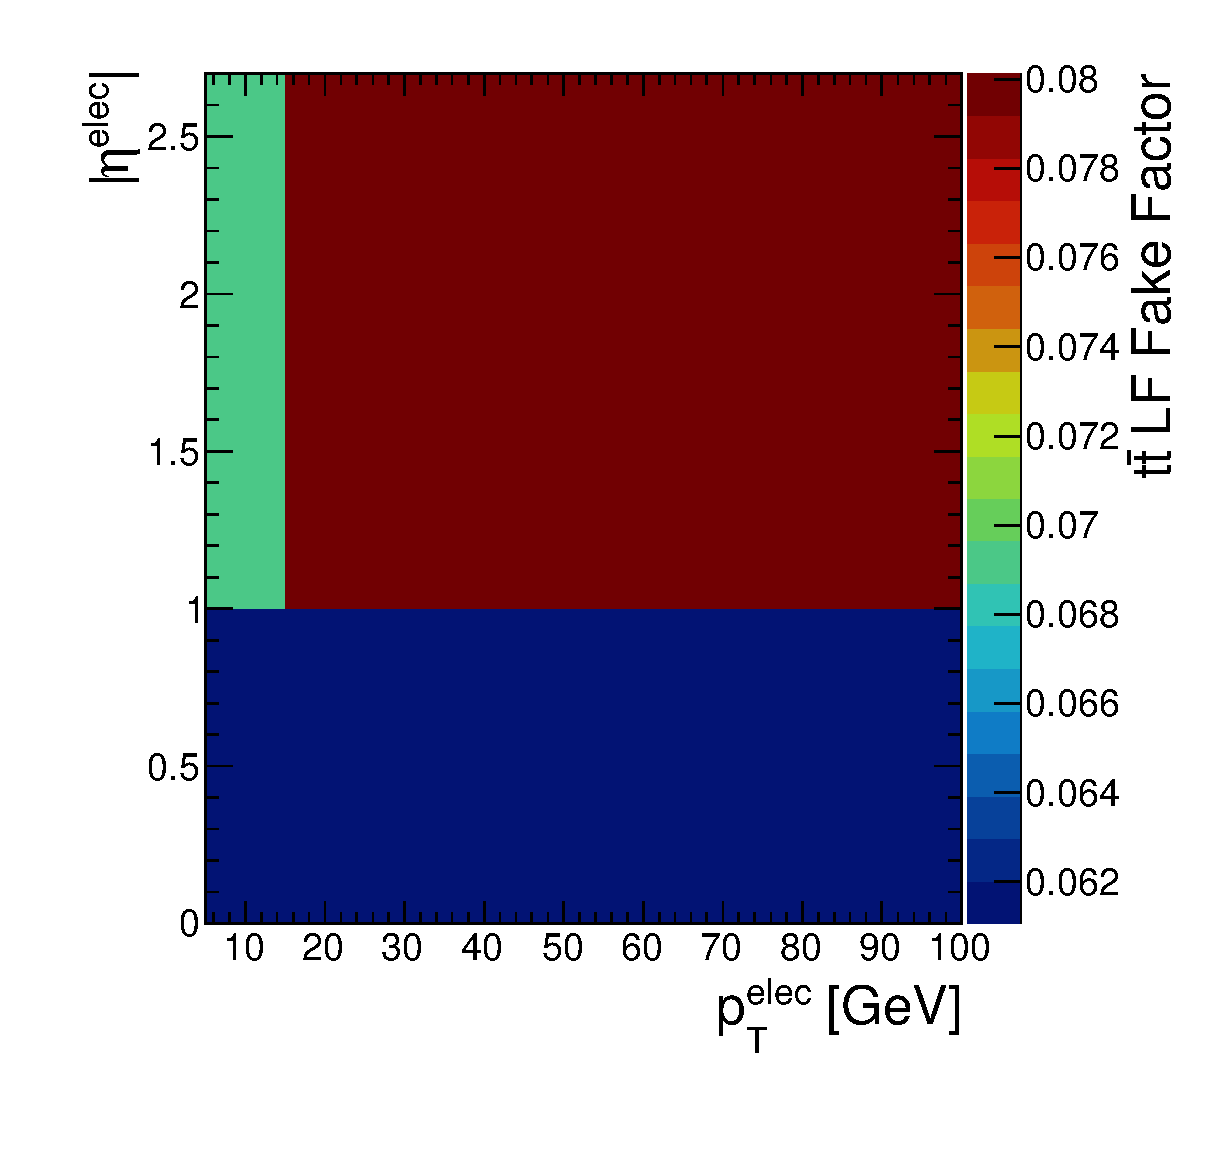
\includegraphics[width=\textwidth]{figs/ff/fakeRatioLFEl.eps}
		\caption{$e$ light flavor}
	\end{subfigure}
	~ 
	\begin{subfigure}[b]{0.475\textwidth}
	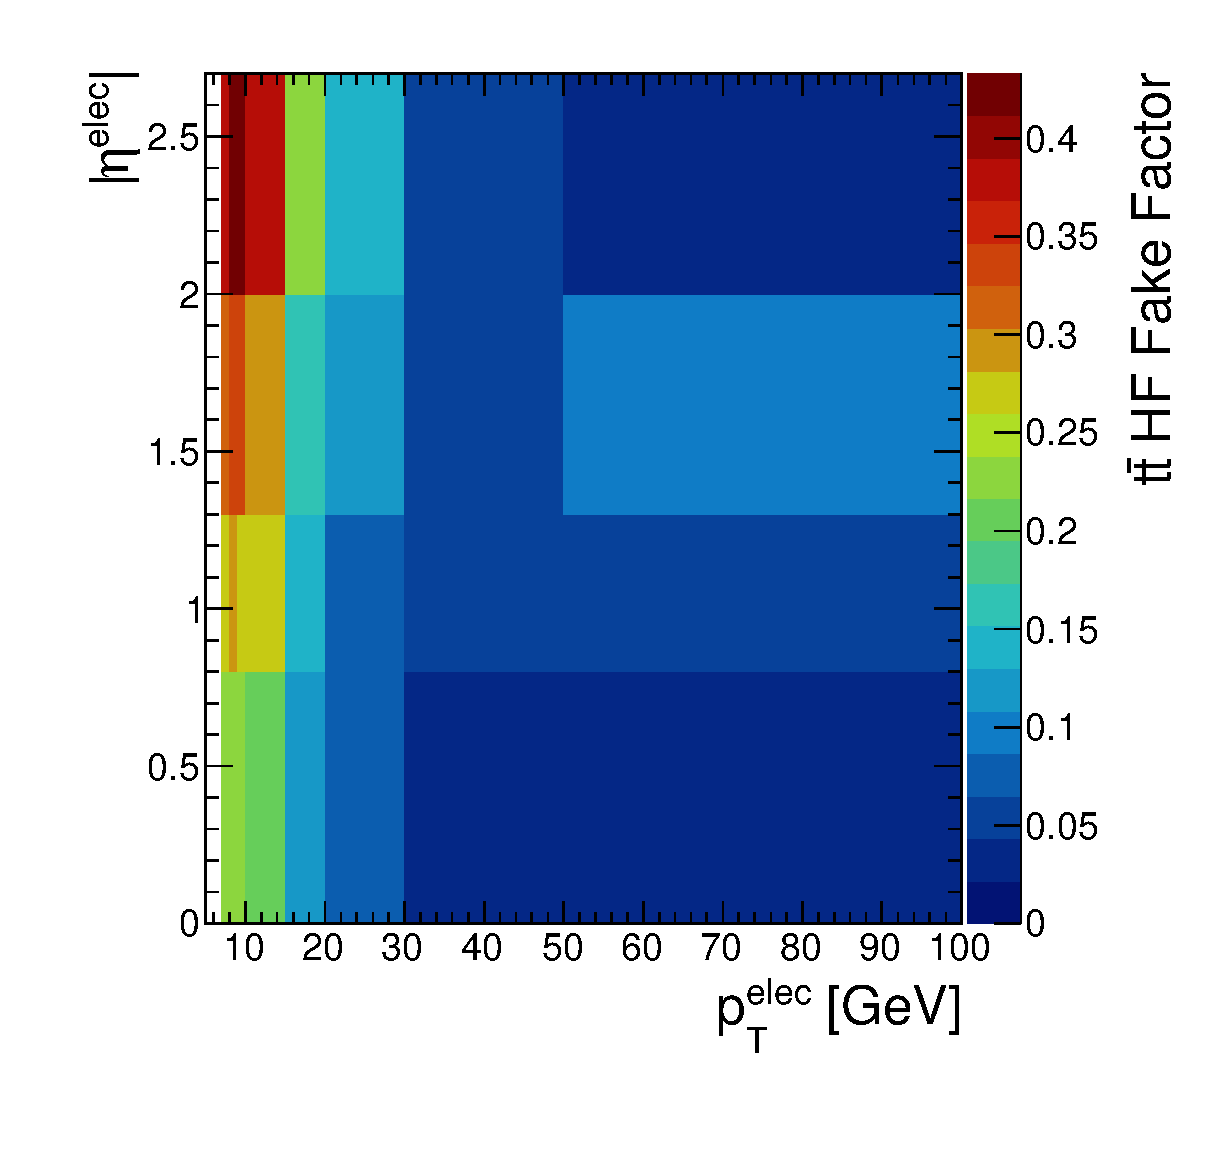
\includegraphics[width=\textwidth]{figs/ff/fakeRatioHFEl.eps}
	\caption{$e$ heavy flavor}
	\end{subfigure}
	~ 
	\begin{subfigure}[b]{0.475\textwidth}
	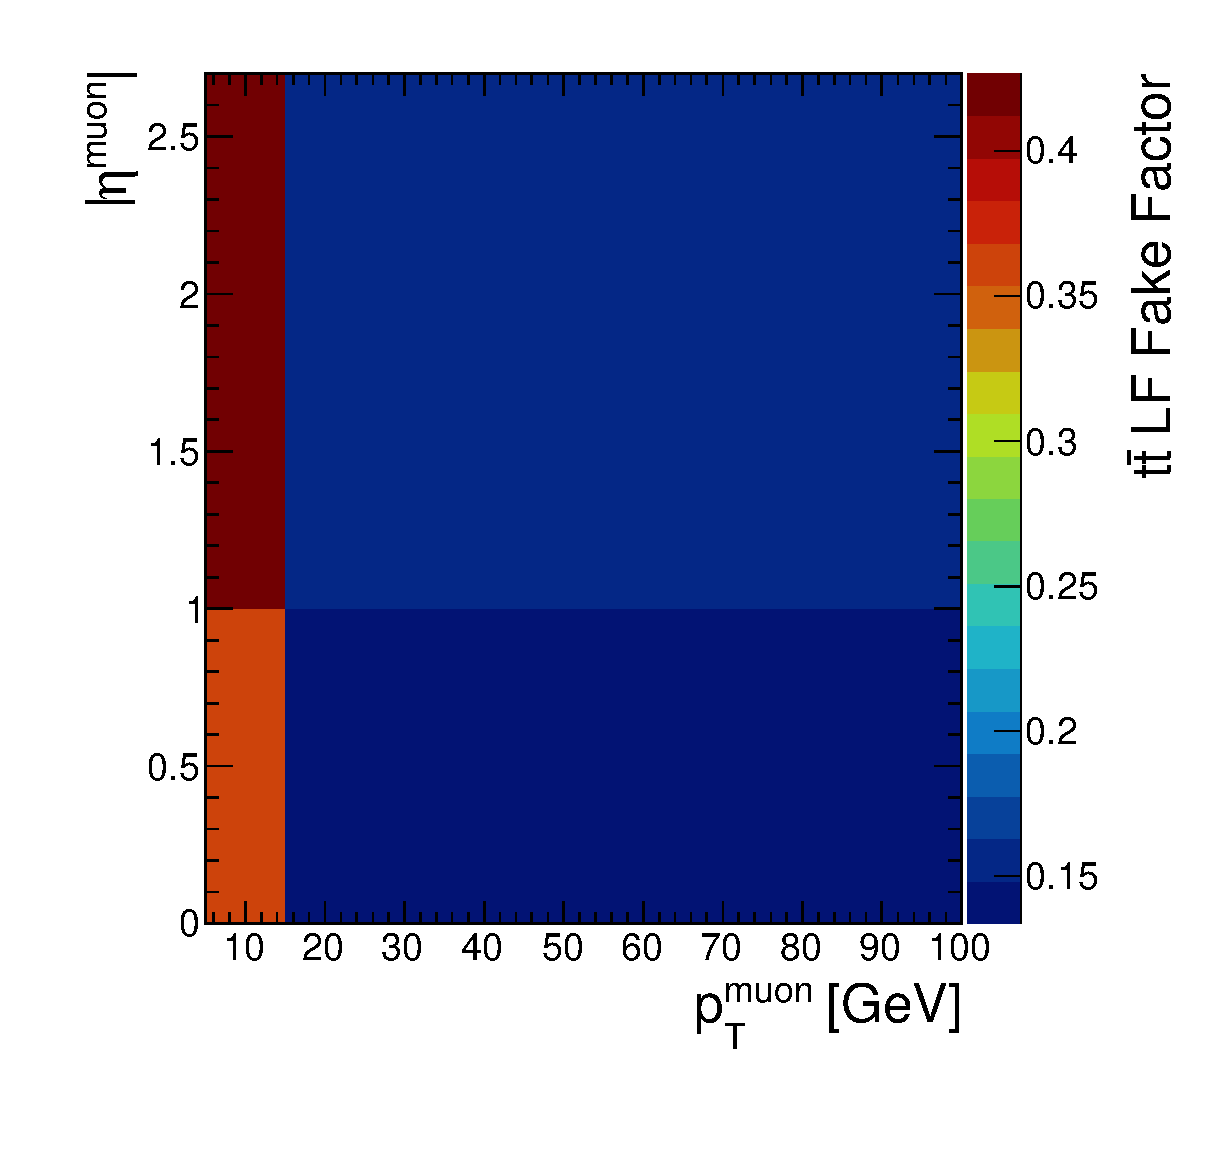
\includegraphics[width=\textwidth]{figs/ff/fakeRatioLFMu.eps}
	\caption{$\mu$ light flavor}
	\end{subfigure}
	~ 
	\begin{subfigure}[b]{0.475\textwidth}
	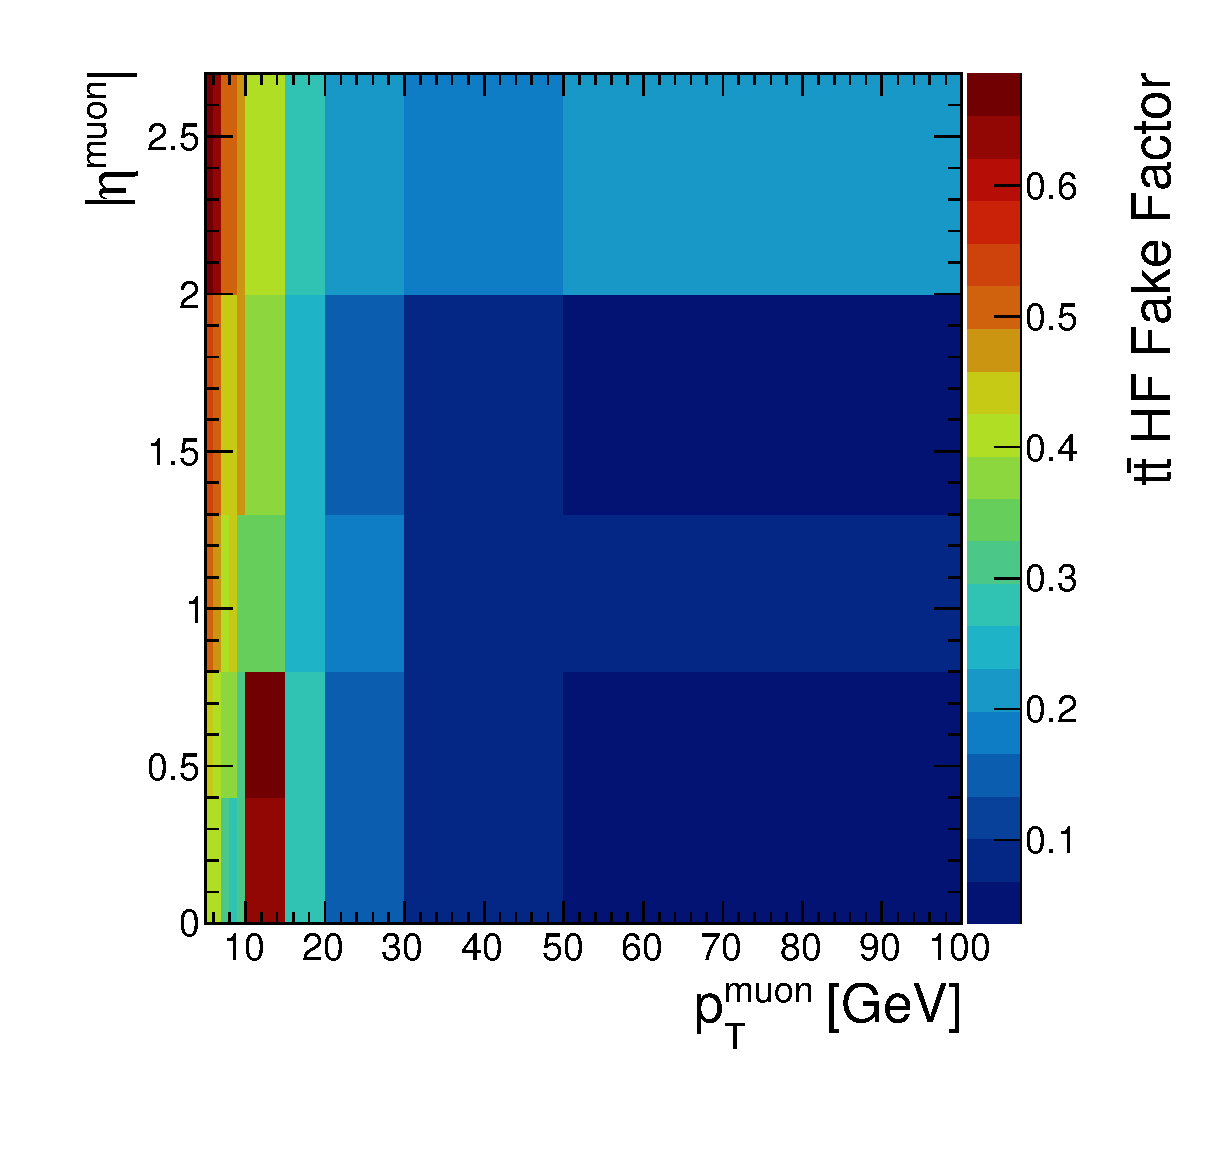
\includegraphics[width=\textwidth]{figs/ff/fakeRatioHFMu.eps}
	\caption{$\mu$ heavy flavor}
	\end{subfigure}
	\caption{Fake factors for electrons and muons in simulated $t\bar{t}$ events as function of their reconstructed $\pt$ and $\eta$.		
		The binning is chosen to give roughly equal statistics in each bin.
	The muon HF fake factor is larger in the $\pt=10-15~\text{GeV}$ bin than surrounding bins due to the isolation requirement for signal muons.}\label{fig:FF-LL}
\end{figure}

\begin{figure}[hp]
	\centering
	\begin{subfigure}[b]{0.475\textwidth}
		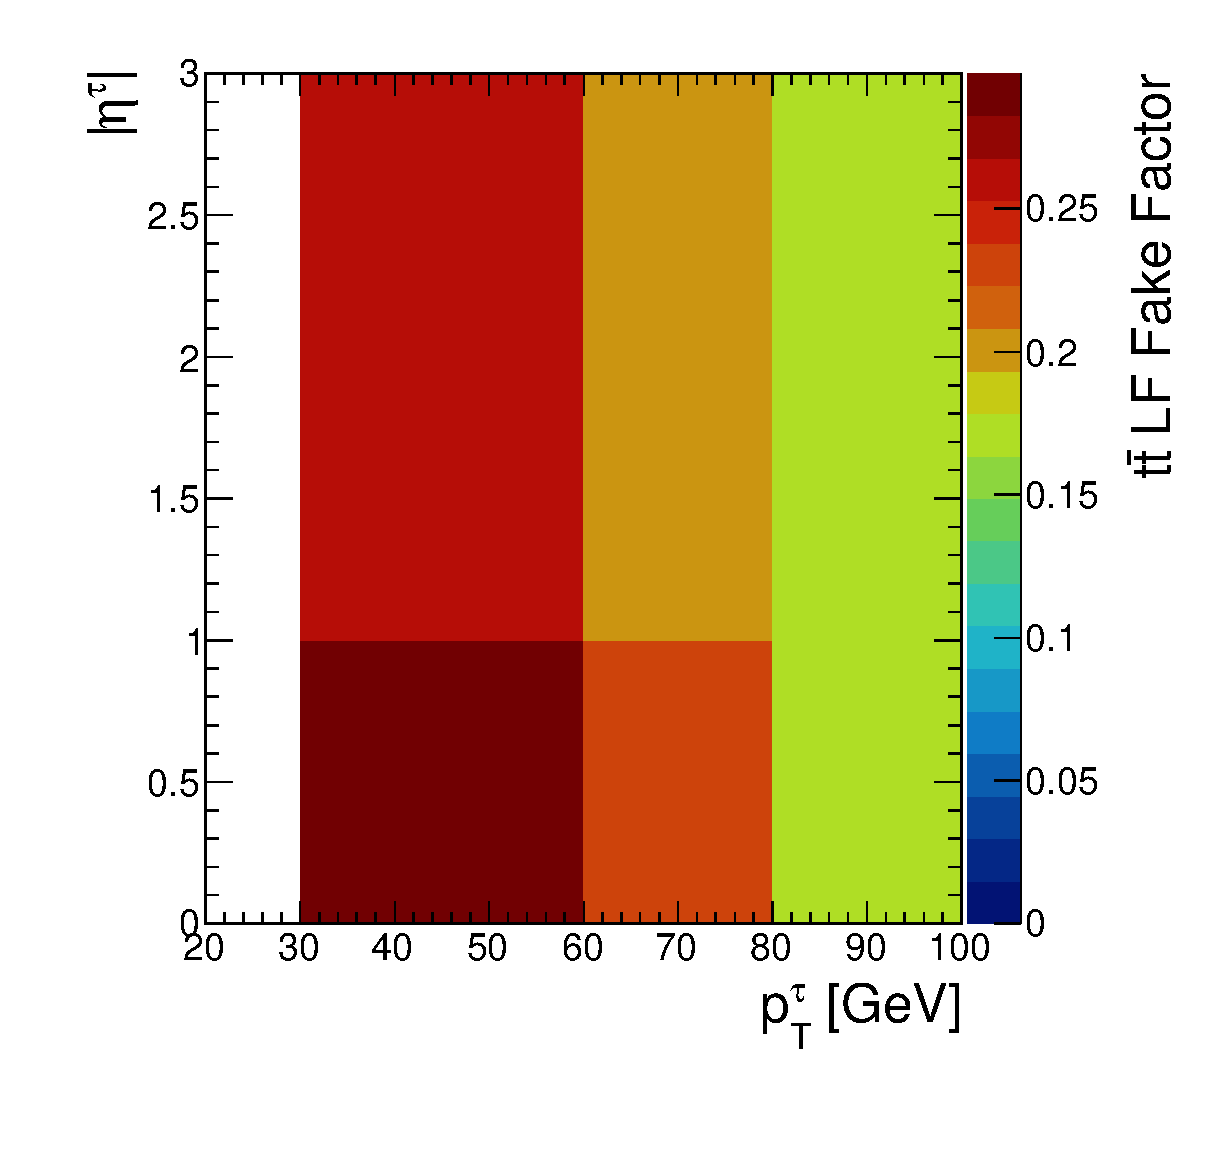
\includegraphics[width=\textwidth]{figs/ff/fakeRatio1pLFTau.eps}
		\caption{light flavor jets}
	\end{subfigure}
	~ 
	\begin{subfigure}[b]{0.475\textwidth}
		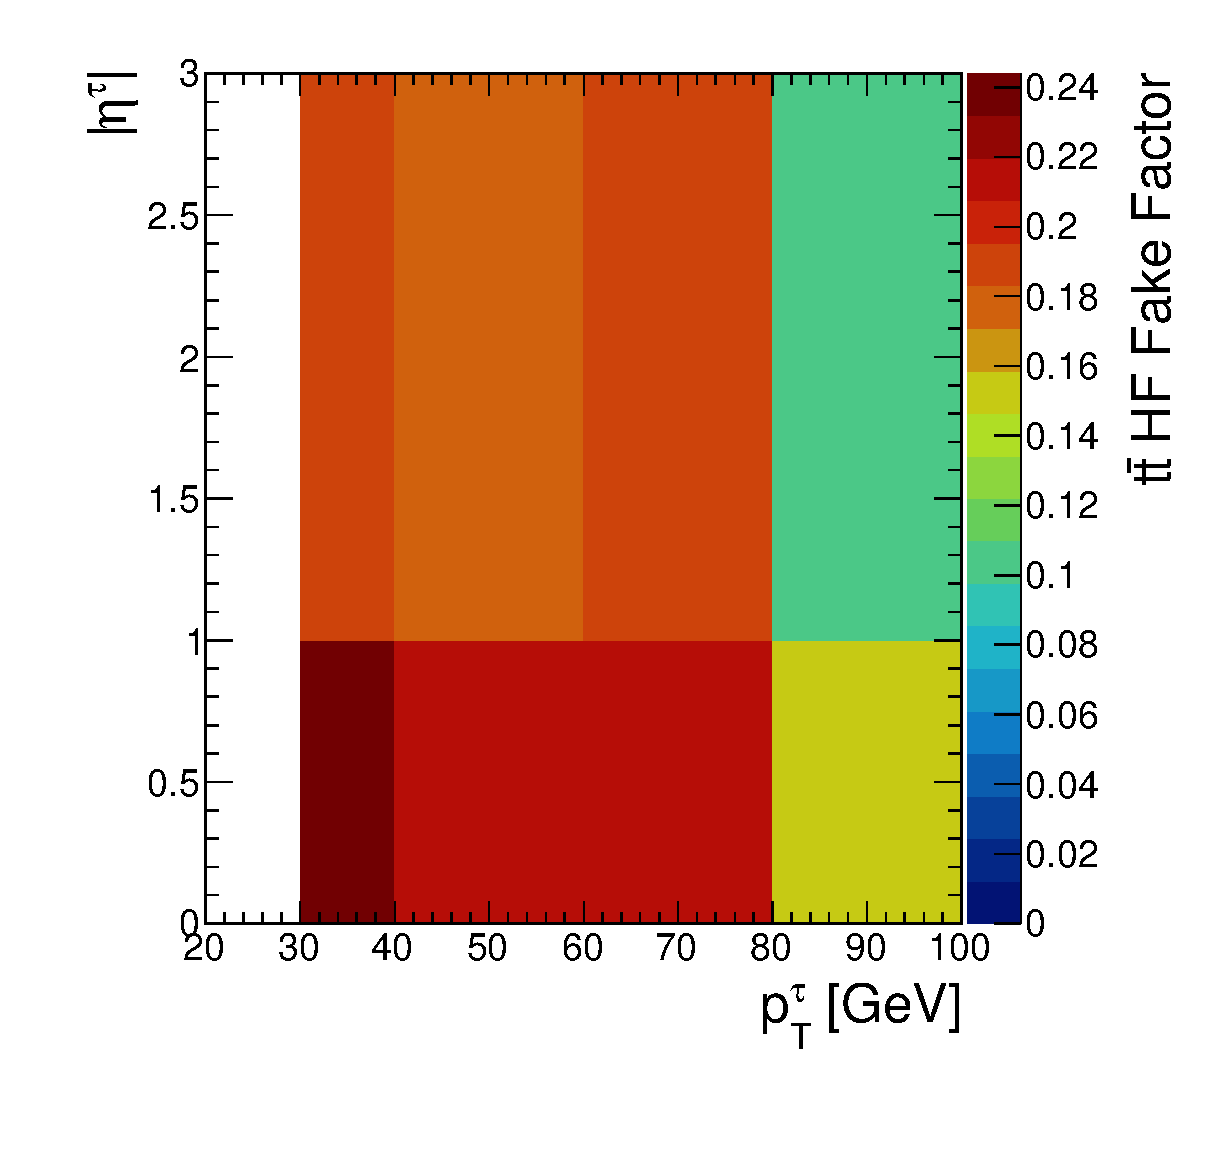
\includegraphics[width=\textwidth]{figs/ff/fakeRatio1pHFTau.eps}
		\caption{heavy flavor jets}
	\end{subfigure}
	~ 
	\begin{subfigure}[b]{0.475\textwidth}
		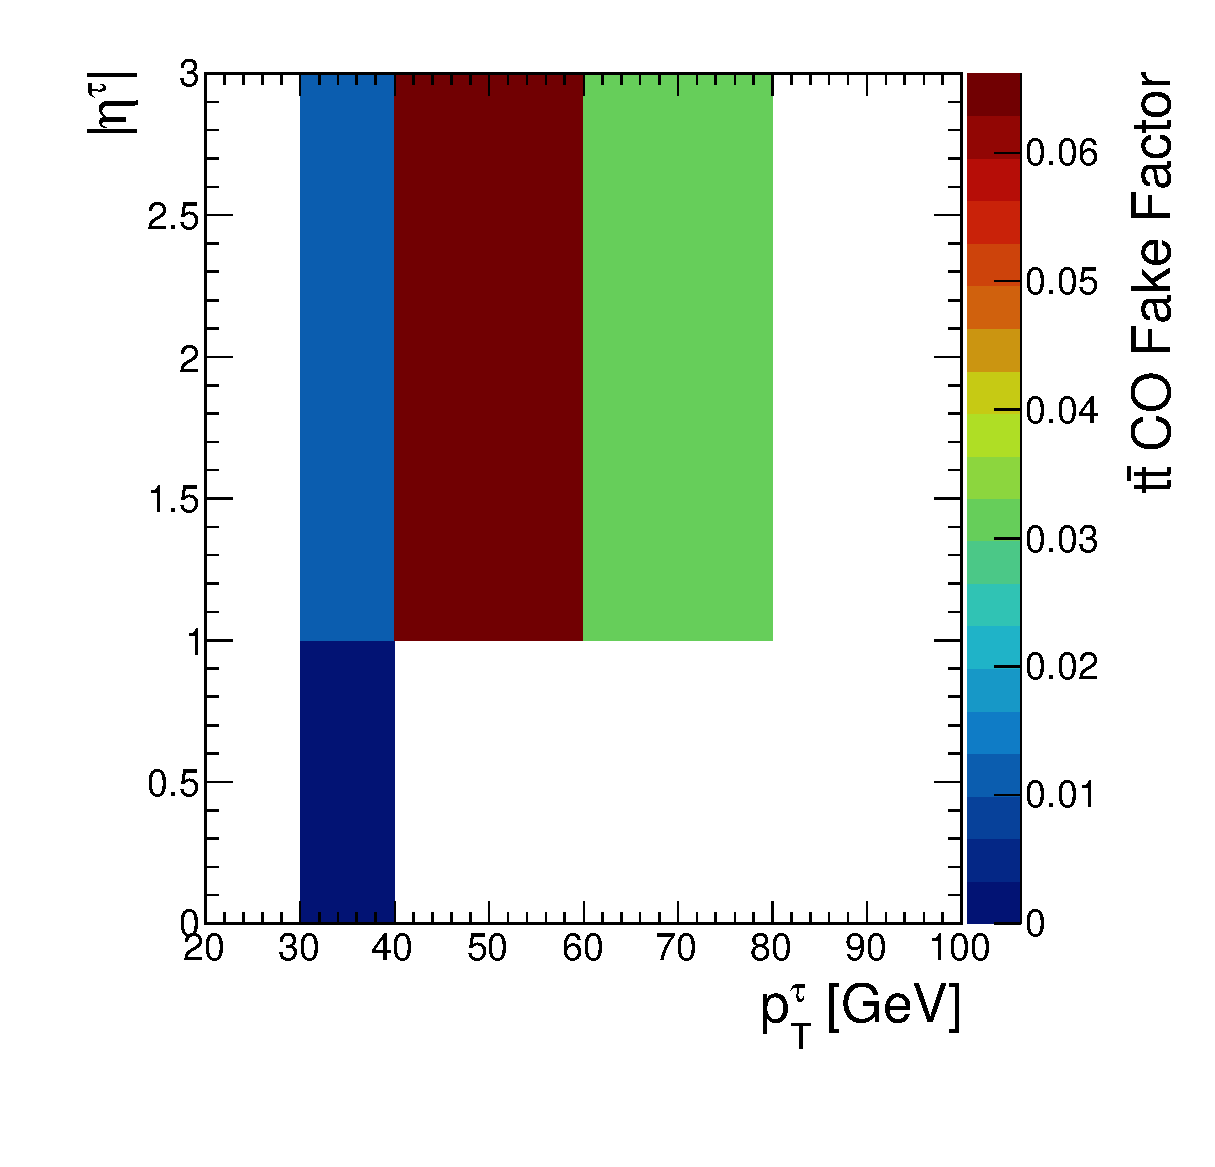
\includegraphics[width=\textwidth]{figs/ff/fakeRatio1pCOTau.eps}
		\caption{photon conversion}
	\end{subfigure}
	~ 
	\begin{subfigure}[b]{0.475\textwidth}
		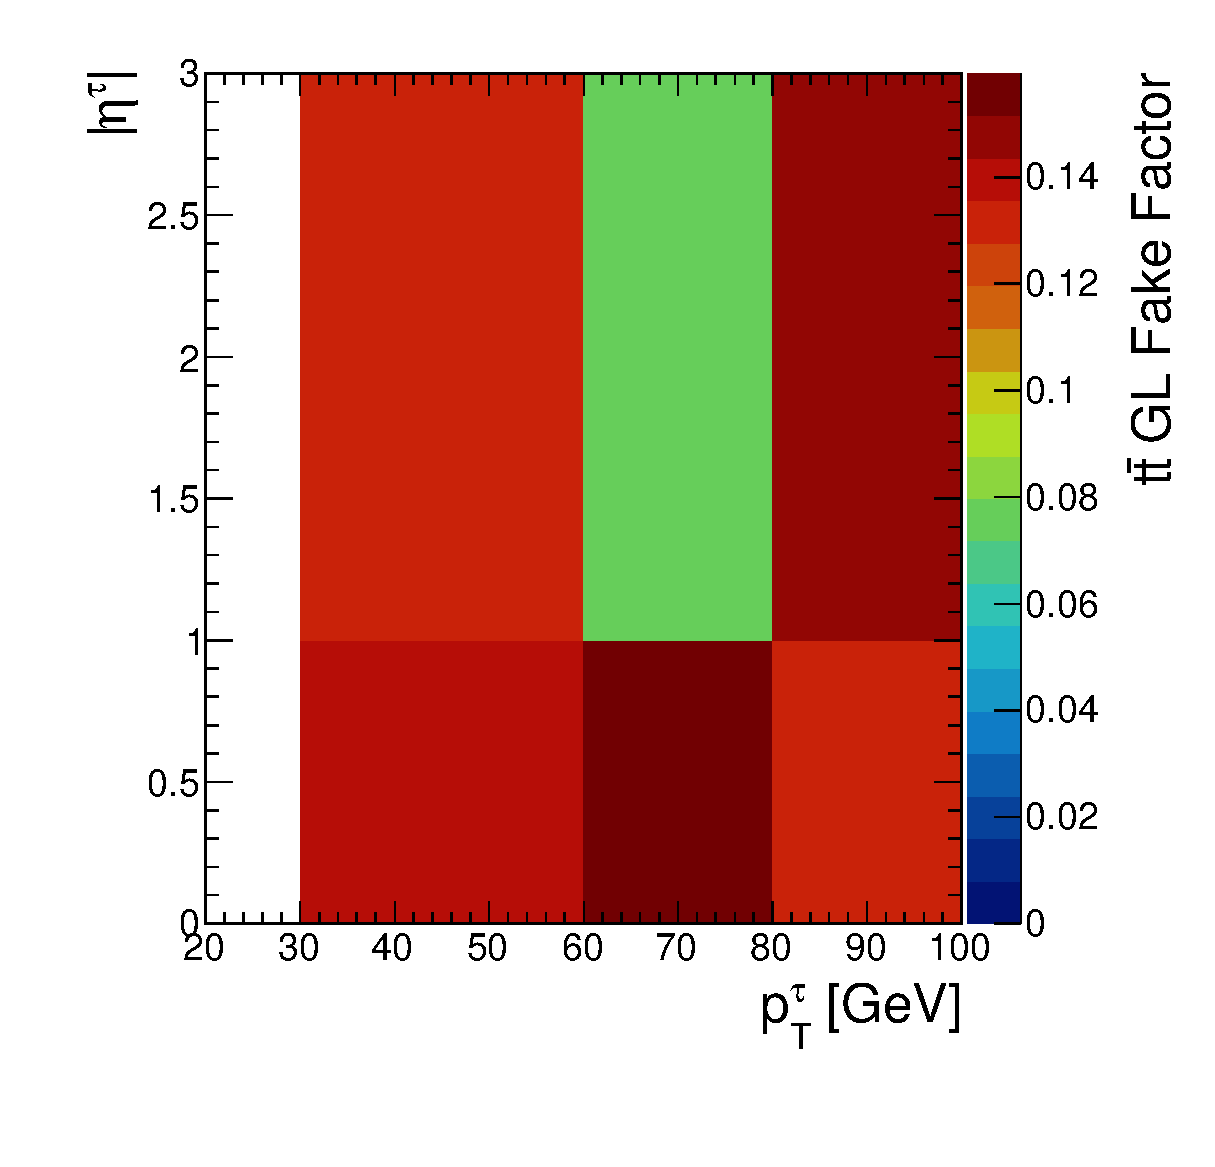
\includegraphics[width=\textwidth]{figs/ff/fakeRatio1pGLTau.eps}
		\caption{gluon-induced jets}
	\end{subfigure}
	\caption{Fake factors for 1-prong hadronically decaying taus in simulated $t\bar{t}$ events. The binning is chosen to give roughly equal statistics in each bin.}\label{fig:FF-TAU}
\end{figure}

\subsubsection{Systematic uncertainties}
Several sources of systematic uncertainty are considered for the SM background estimates and signal yield predictions. The systematic uncertainties affecting the simulation-based estimate can be divided into three components: MC statistical uncertainty, sources of experimental uncertainty 
(from identified physics objects $e$, $\mu$, $\tau$ and jets, and also $E_\mathrm{T}^\text{miss}$), and sources of theoretical uncertainty. The reducible
background is affected by different sources of uncertainty associated with data counts in control regions and uncertainties in the weighted fake factors.
The MC statistical uncertainty for the simulation-based background estimate is small and less than 7\% of the total background estimate in all signal regions.
Systematic uncertainties in the SUSY signal yields from experimental and theoretical sources are typically of the order of 10\% each.

\subsection{Results}

In general, the observed yields in each signal region  are found to be consistent with the SM expectations within a local significance of at most $\sim 1 \sigma$.
% An excess of data of $2.3\sigma$ is, however, seen in SR0D.

In order to quantify the probability for the background-only hypothesis to fluctuate to the observed number of events or higher, a one-sided $p_0$-value is calculated using pseudo-experiments, where the profile likelihood ratio is used as a test statistic to exclude the signal-plus-background hypothesis. A signal model can be
excluded at 95\% confidence level (CL) if the $\mathrm{CL}_\mathrm{s}$ of the signal-plus-background hypothesis is below
0.05. The 95\% CL upper limits on the signal cross section times efficiency and the $\mathrm{CL}_\mathrm{b}$ value for the background-only
hypothesis are also calculated for each signal region.

The number of observed events in each signal region is used to set exclusion limits in the SUSY models, where the statistical combination of all disjoint signal regions is used. 
Since SR0A and SR0B are overlapping signal regions, the one with the better expected exclusion is used in the combination. For the exclusion limits, the observed and expected 95\% CL limits are calculated by performing pseudo-experiments for each SUSY model point, taking into account the theoretical and experimental uncertainties in the SM background and the experimental uncertainties in the signal. For all expected and observed exclusion limit contours, the $\pm 1 ~\sigma_\mathrm{exp}$  uncertainty band indicates the impact on the expected limit of the systematic and statistical uncertainties included in the fit. The $\pm 1 ~\sigma_\mathrm{theory}^\mathrm{SUSY}$ uncertainty lines around the observed limit illustrate the change in the observed limit as the nominal signal cross section is scaled up and down by the theoretical cross section uncertainty.


\begin{figure}[t]
 \centering
 \begin{subfigure}[b]{0.48\textwidth}
  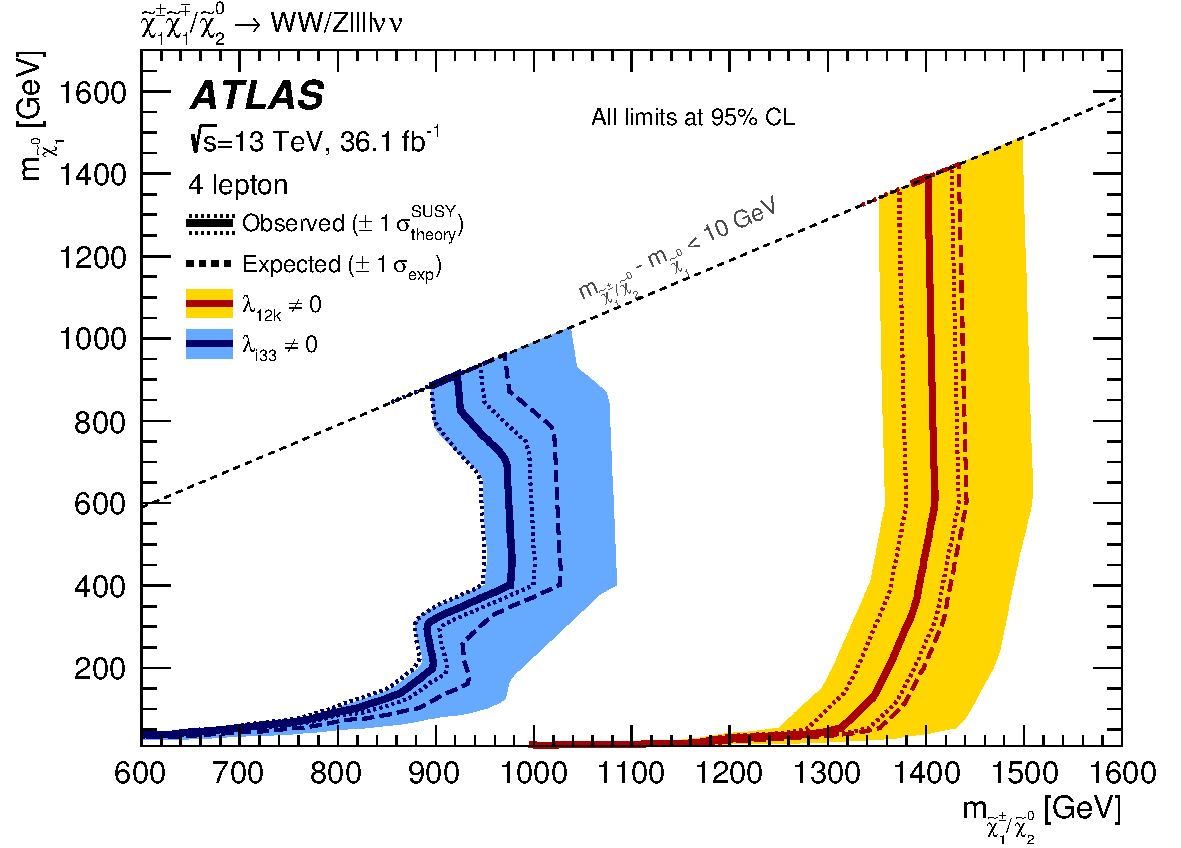
\includegraphics[width=\textwidth]{figs/fig_07a.pdf}
  \caption{Wino W/Z NLSP}
 \end{subfigure}
 ~ 
 \begin{subfigure}[b]{0.48\textwidth}
  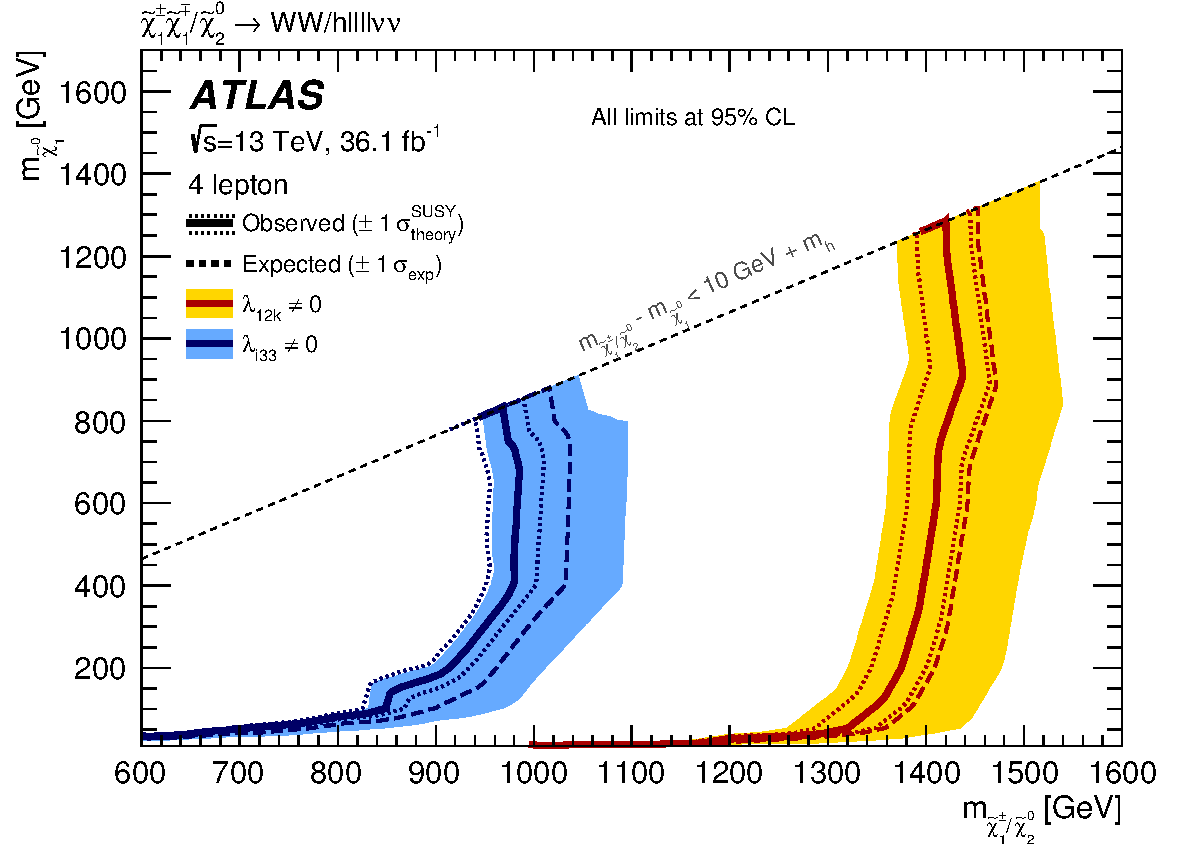
\includegraphics[width=\textwidth]{figs/fig_07b.pdf}
  \caption{Wino W/h NLSP}
  \label{fig:fig_07b}
 \end{subfigure}
 ~ 
 \begin{subfigure}[b]{0.48\textwidth}
  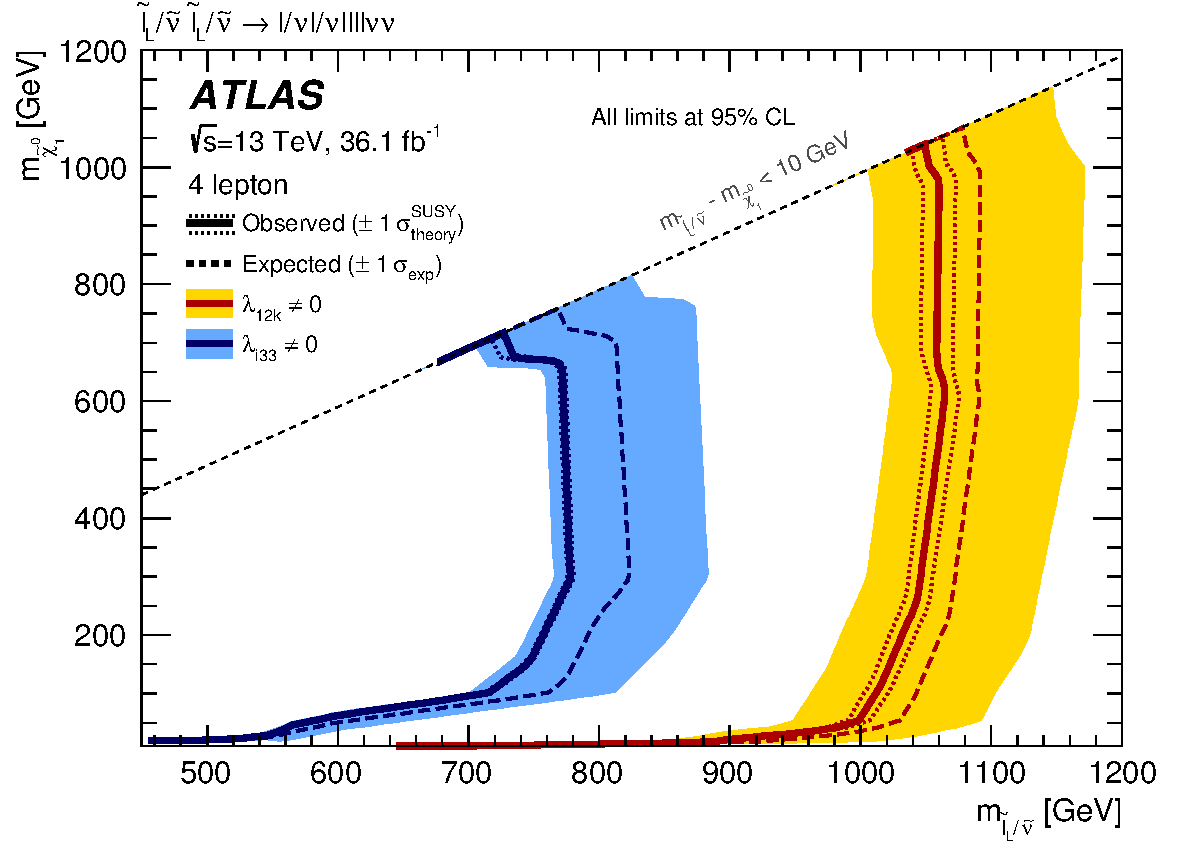
\includegraphics[width=\textwidth]{figs/fig_08a.pdf}
  \caption{Slepton/sneutrino NLSP}
 \end{subfigure}
 ~
 \begin{subfigure}[b]{0.48\textwidth}
  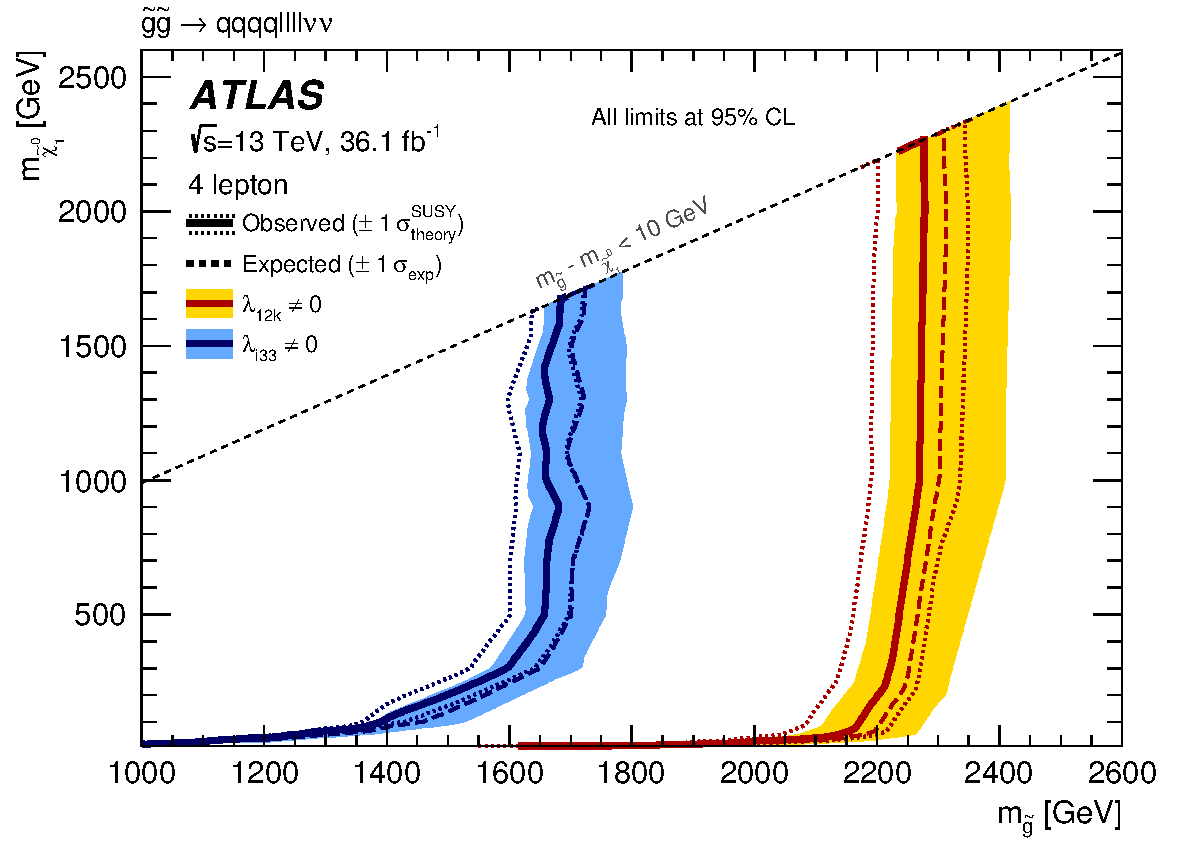
\includegraphics[width=\textwidth]{figs/fig_08b.pdf}
  \caption{Gluino NLSP}\label{fig:excl-gluino}
 \end{subfigure}
 \caption{Expected (dashed) and observed (solid) 95\% CL exclusion limits on the SUSY RPV models considered in the analysis. The limits are set using the statistical combination of disjoint signal regions. Where the signal regions are not mutually exclusive, the observed $\mathrm{CL}_s$ value is taken from the signal region with the better expected $\mathrm{CL}_s$  value~\cite{Aaboud:2018zeb}. }\label{fig:RPV-limits}
\end{figure}
Figure~\ref{fig:RPV-limits} shows the exclusion contours for the RPV models considered in the search. The exclusion limits in the RPV models extend to high masses due to the high lepton multiplicity in these scenarios and the high efficiency of the $m_\mathrm{eff}$ selections. Wino-like $\tilde{\chi}_1^\pm/\tilde{\chi}_2^0$, slepton/sneutrino and gluino masses  up to $1.46$~TeV, $1.06$~TeV, and $2.25$~TeV are excluded, respectively.

The results are also interpreted in simplified higgsino GGM models, where higgsino-like $\tilde{\chi}_1^\pm/\tilde{\chi}_2^0/\tilde{\chi}_1^0$ masses up to 295 GeV are excluded in scenarios with a 100\% branching ratio for $\tilde{\chi}_1^0$ decay to a Z boson and a gravitino (Figure~\ref{fig:RPC-limits}).
\begin{figure}[htbp]
 \centering
 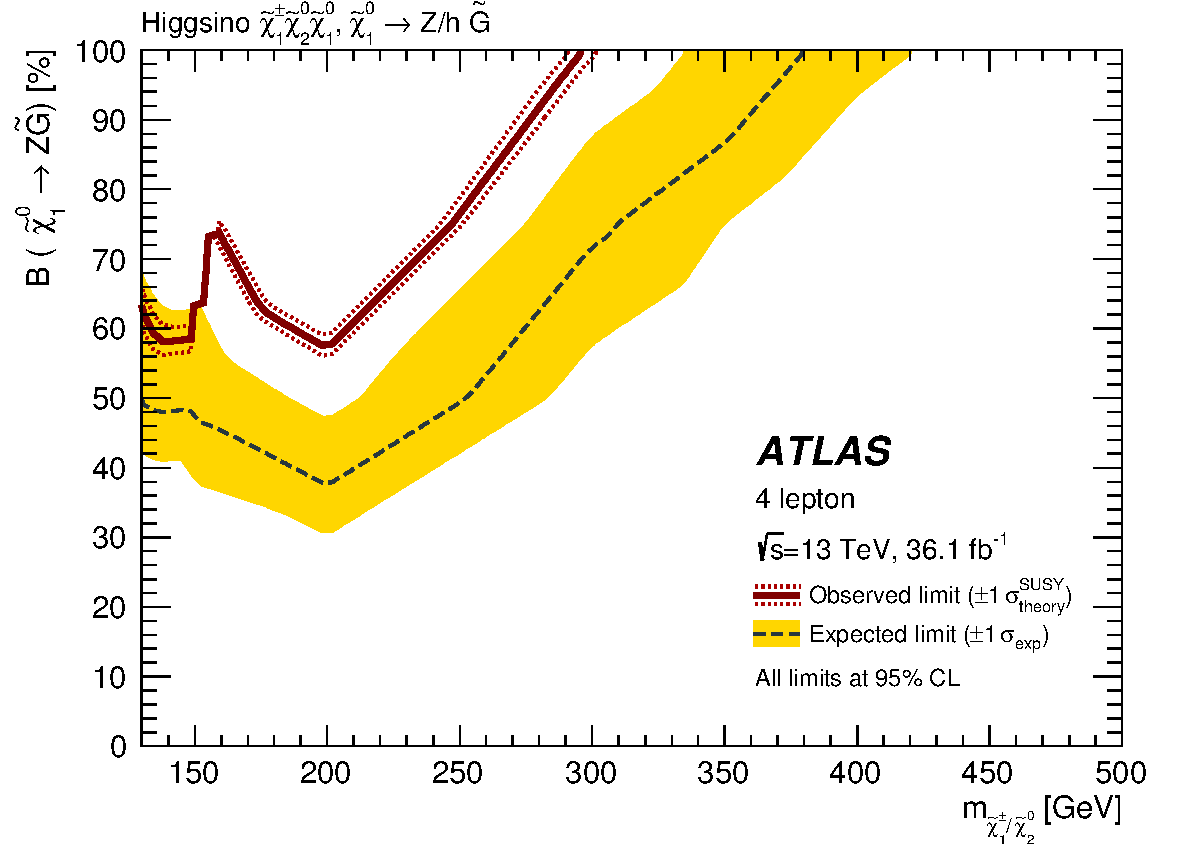
\includegraphics[width=0.8\textwidth]{figs/fig_09.pdf}
\caption{Expected (dashed) and observed (solid) 95\% CL exclusion limits on the GGM higgsino model considered in the analysis. The limits are set using the statistical combination of disjoint signal regions. Where the signal regions are not mutually exclusive, the observed $\mathrm{CL}_s$ value is taken from the signal region with the better expected $\mathrm{CL}_s$ value~\cite{Aaboud:2018zeb}. }\label{fig:RPC-limits}
\end{figure}
 
\begin{figure}[h]
	\centering
	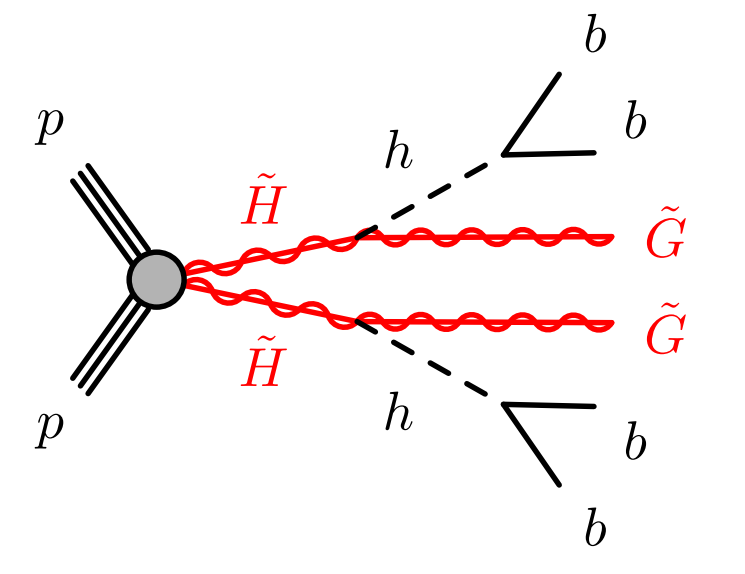
\includegraphics[width=0.4\linewidth]{figs/hino-feyn}
	\caption{Diagram for the higgsino ($\tilde{H}$) production and decay. The production occurs via mass-degenerate pairs of charginos or neutralinos, which decay to the $\tilde{\chi}_1^0$ and typically low-momentum b-quarks.}
	\label{fig:hino-feyn}
\end{figure}
Searches for higgsinos within gauge-mediated scenarios can be performed in final states with different decay products as well, such as b-flavor jets, as illustrated in Figure~\ref{fig:hino-feyn}.
ATLAS performed such kind of search in events containing missing transverse momentum and several energetic jets, at least three of which must be identified as b-quark jets~\cite{Aaboud:2018htj}. As no significant excess is found above the predicted background, limits on the cross-section are set as a function of the mass of the higgsino  in simplified models assuming production via mass-degenerate higgsinos decaying to a Higgs boson and a gravitino. Higgsinos with masses between 130 and 230 GeV and between 290 and 880 GeV are excluded at the 95\% confidence level. Interpretations of the limits in terms of the branching ratio of the higgsino to a Z boson or a Higgs boson are also presented, and a 45\% branching ratio to a Higgs boson is excluded for higgsino masses of about 400 GeV.
\begin{figure}[htbp]
 \centering
 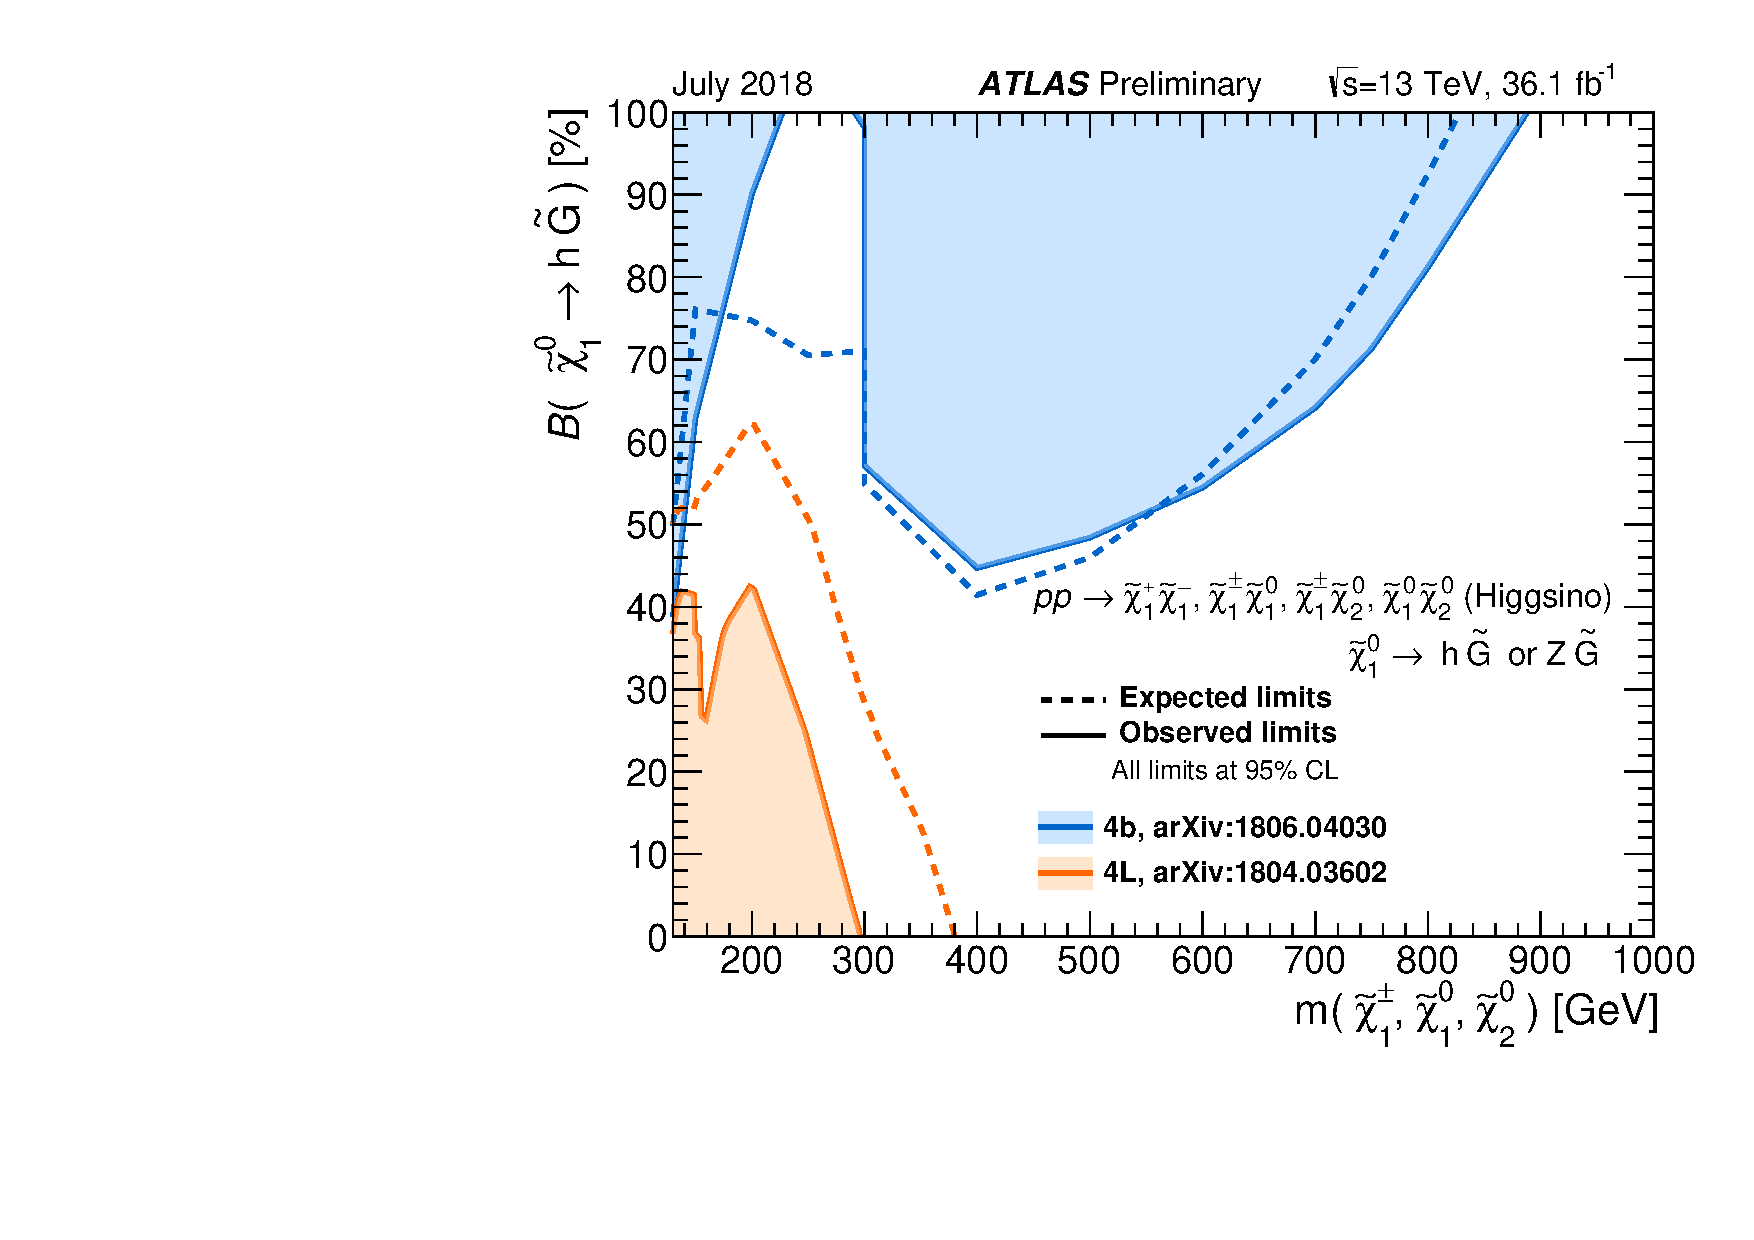
\includegraphics[width=0.8\linewidth]{figs/fig_Hino}
 \caption{The 95\% CL exclusion limits on the GGM model involving higgsino triplets~\cite{ATL-PHYS-PUB-2019-022}. The model assumes a pure higgsino NLSP that promptly decays to either Z + gravitino or Higgs + gravitino, and subsequently decaying into charged leptons or b-quarks. The limits are displayed as a function of the mass of the nearly mass-degenerate higgsino triplet and the branching fraction of lightest higgsino to Higgs gravitino. This contour plot combines the limit results from the four-lepton~\cite{Aaboud:2018zeb} and multi-b-jet~\cite{Aaboud:2018htj} searches.
 In the range $200~\mathrm{GeV} < m_\text{higgsino} < 300~\mathrm{GeV}$, 
 the observed limit is $1-2~\sigma$ weaker than expected due to the data exceeding the background in several bins with $E_T^\text{miss} > 100$~GeV 
 in the low-mass regions of the analysis.
}
 \label{fig:fig_Hino}
\end{figure}

The limit results of the two higgsinos searches in final states with multiple charged leptons or b-flavor jets are combined in the contour plot shown in Figure~\ref{fig:fig_Hino}. As seen, the multi-lepton analysis has more sensitivity to higgsino decays via the Z-boson, while the multi-b-jet search shows more sensitivity to higgsino decays occurring via the Higgs boson emission expanding to considerably higher higgsino masses.

\subsection{Comparison with CMS}
The CMS collaboration also presented in Ref.~\cite{PhysRevD.97.032007} a search for higgsinos in events with missing transverse momentum greater than 150 GeV and at least three jets identified as originating from b-quark hadronization. 
In each event, two Higgs boson candidates are reconstructed with each one decaying as $H \to bb$. 
Search regions within a Higgs boson mass window are defined in order to be sensitive to final states with 2 pairs of b-tagged jets associated with substantially large missing transverse momentum.

The CMS data sample corresponds to an integrated luminosity of $35.9~\mathrm{fb}^{-1}$ at $\sqrt{s} = 13$~TeV, similar to the ATLAS analysis. 
Because the signal has four b-quarks, while the background is dominated by $t\bar{t}$ events containing only two bottom quarks from the top quark decays, 
CMS binned the analysis according to the number of b-tagged jets. 
In each event, the mass difference between the two Higgs boson candidates is required to be small, and the average mass of the two candidates is
used in conjunction with the number of observed b-quark tags to define signal and sideband regions.
The observed event yields in these regions are used to obtain estimates for the SM background in the signal regions without input from simulated event samples. 
The data are also binned in regions of missing transverse momentum to enhance the sensitivity to the signal.
The observed event yields in the signal regions are consistent with the background predictions.

\begin{figure}[ht]
	\centering
	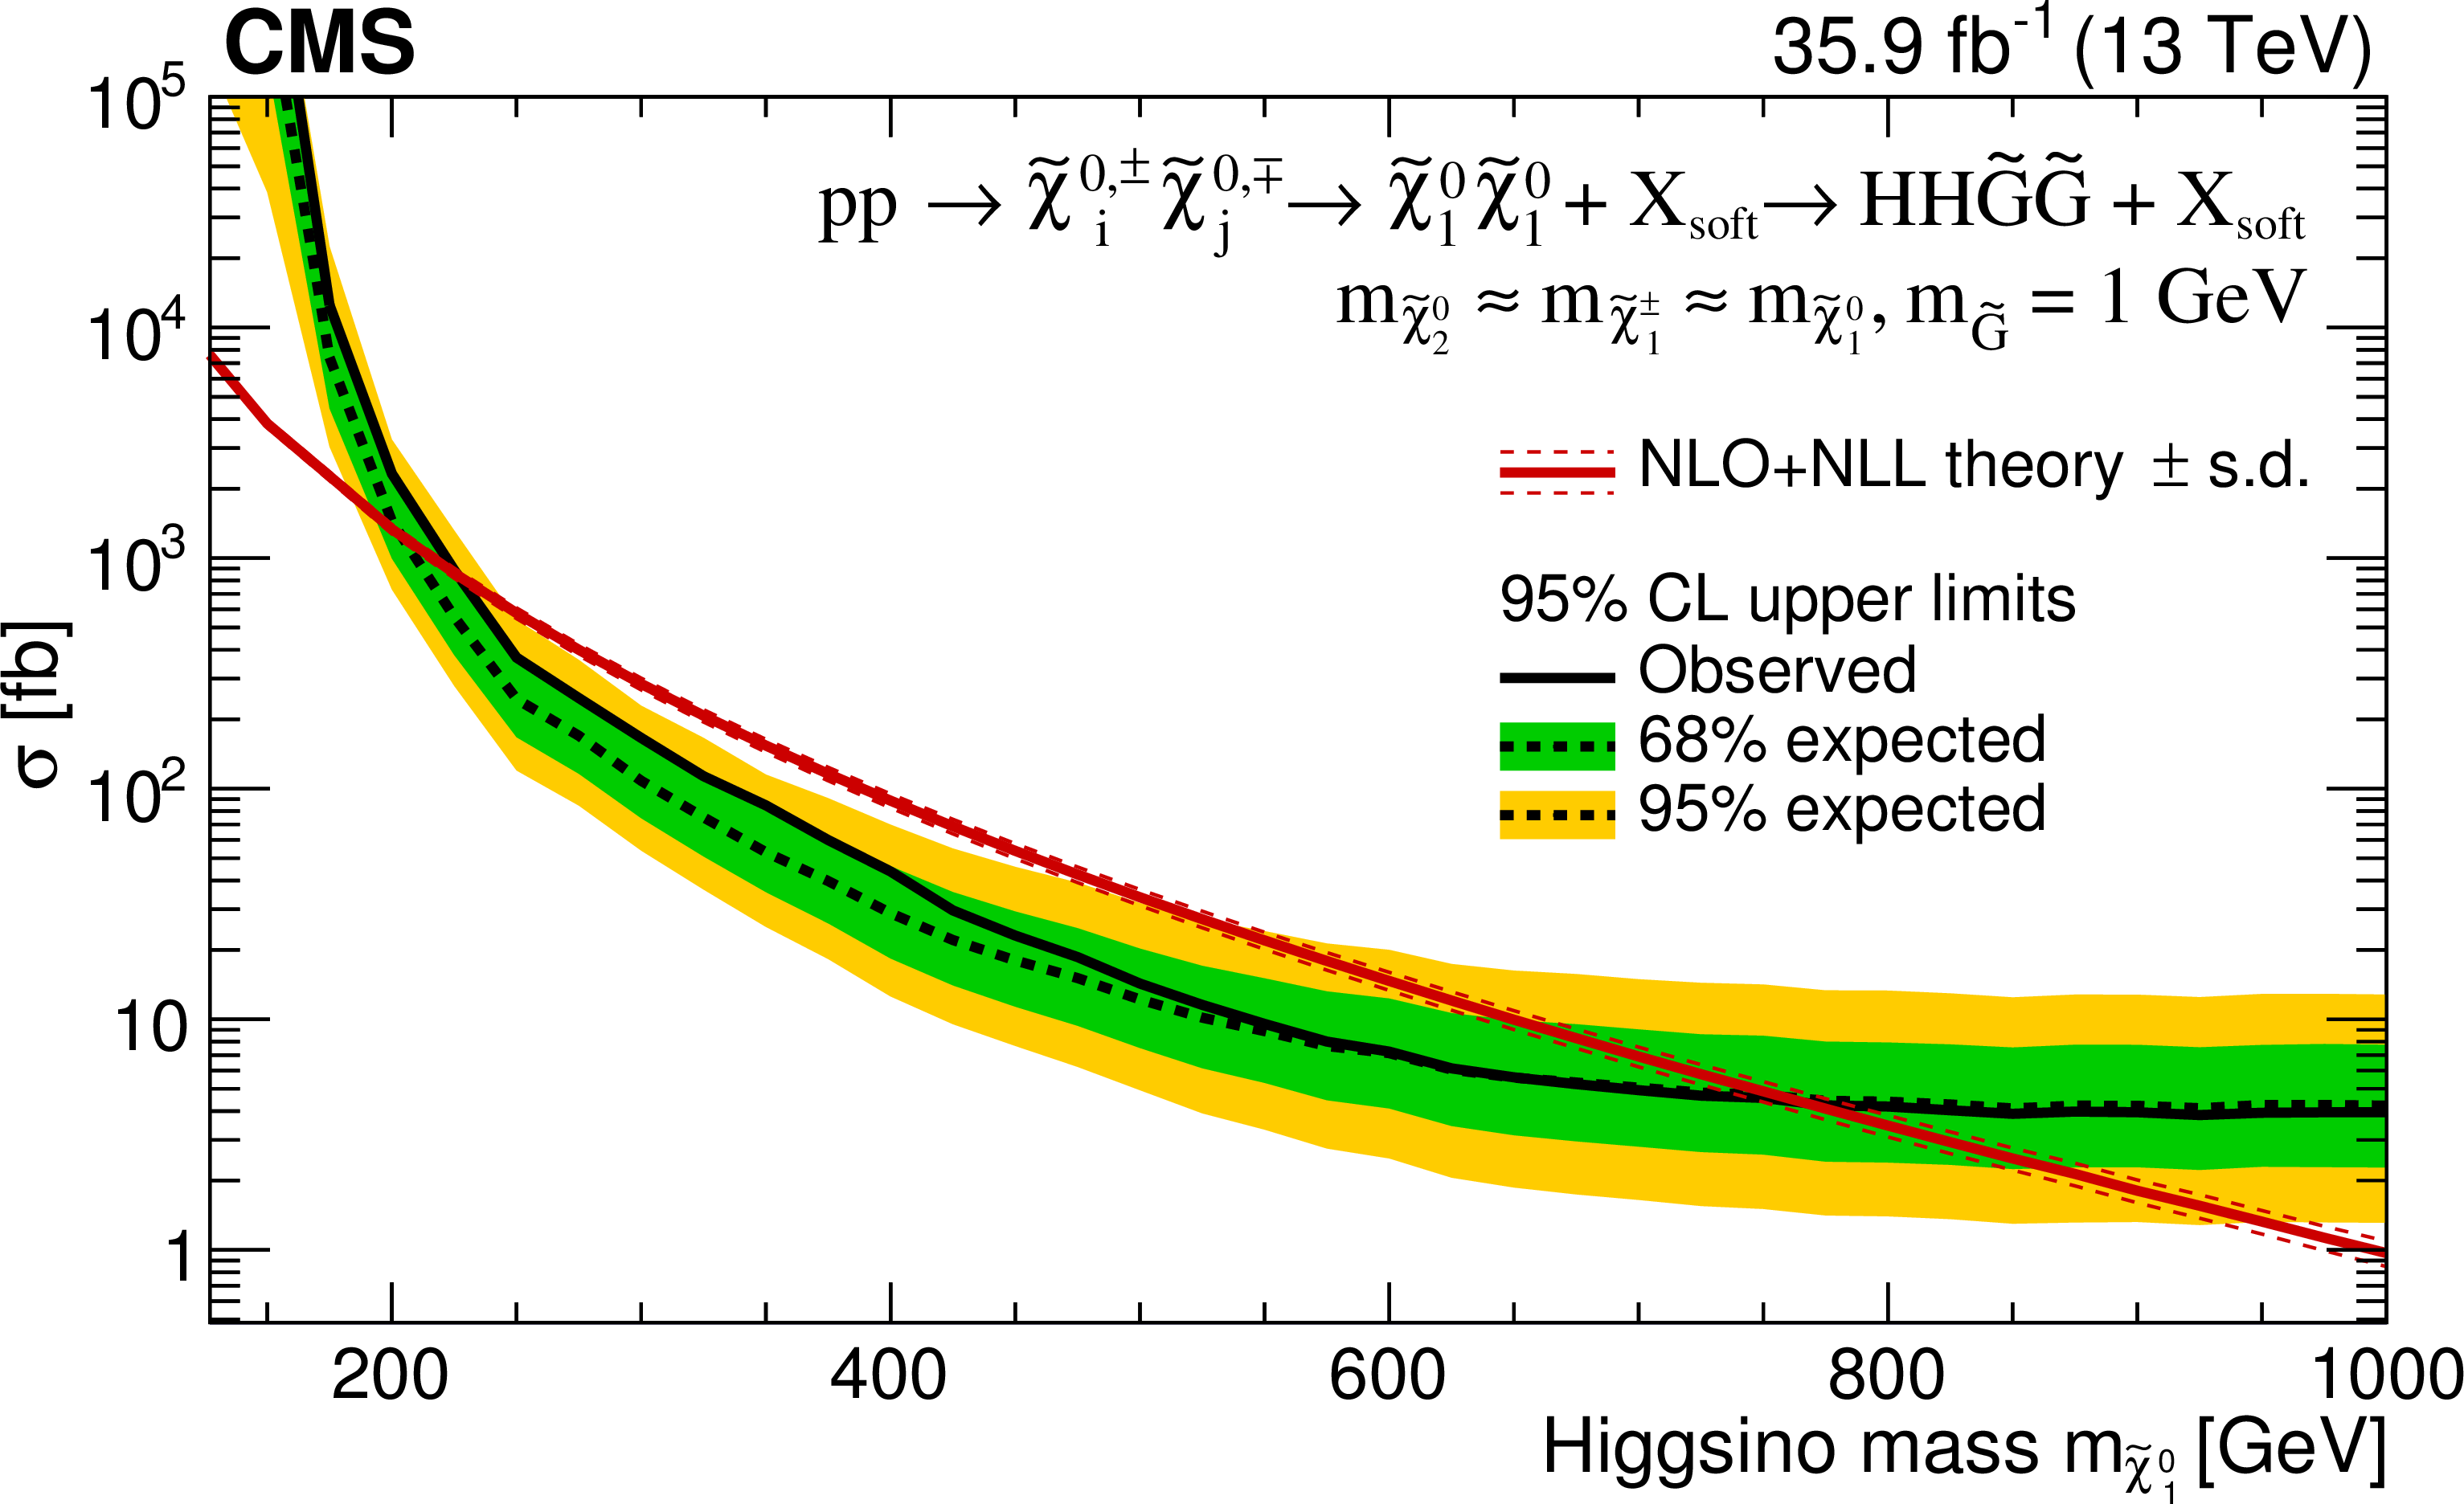
\includegraphics[width=0.7\linewidth]{figs/CMS-SUS-16-044_Figure_009}
	\caption{Expected (dashed black line) and observed (solid black line) excluded cross sections at 95\% CL as a function of the higgsino mass. The theoretical cross section for the higgsino simplified model is shown as the red solid line. Adapted from the CMS analysis of Ref.~\cite{PhysRevD.97.032007}.}
	\label{fig:cms-sus-16-044figure009}
\end{figure}

These results are interpreted in the context of a model in which each higgsino decays into a
Higgs boson and a nearly massless LSP, which is weakly interacting. 
Such a scenario is compatible with gauge-mediated supersymmetry breaking models, in which the LSP is a goldstino. 
The cross-section calculation assumes that the higgsino sector is mass degenerate and sums over the cross sections for the pair production of all relevant
combinations of higgsinos, but all decays are assumed to be prompt. 
With the CMS analysis, higgsinos with masses in the range 230 to 770 GeV are excluded at 95\% confidence level. 

The corresponding ATLAS analysis~\cite{Aaboud_2018}, excludes Higgsinos with masses between 130 and 230 GeV and
between 290 and 880 GeV at the 95\% confidence level. ATLAS performs two complementary analyses, targeting high- and low-mass signals to maximize sensitivity.
For the analysis targeting high-mass higgsinos, events are selected using missing transverse energy triggers. 
Events with at least three b-jets are further analyzed, and jet pairs are assigned to two Higgs candidates.
For the low-mass analysis, events are selected with a combination of b-jet triggers, and events with four
b-jets are further analyzed by grouping the jets into Higgs candidates. On the other hand, the CMS analysis defines multiple signal regions in order to optimize signal efficiency and background rejection. In particular, the CMS analysis defines mutually exclusive categories based on the number of b-tagged jets with varying thresholds on the missing transverse momentum.


\subsection{Conclusions}
Results are reported from a search for new physics in the final state with four or more leptons (electrons,muons or taus), using  $pp$ collision data at $\sqrt{s}=13$~TeV collected by the ATLAS
detector at the LHC in 2015 and 2016.
Signal regions are defined with up to two hadronically decaying
taus, and target lepton-rich RPV  SUSY signals with selections requiring large effective mass or
missing transverse momentum, and the absence of reconstructed Z-boson candidates. 
The results are interpreted in simplified models of NLSP pair production with RPV LSP decay and in simplified higgsino GGM models. 
Data yields in the signal regions are consistent with SM expectations and therefore exclusion limits are set at the 95\% confidence level.

In RPV simplified models with decays of the LSP to charged leptons, lower limits of 1.4 TeV, 1.06 TeV, and 2.25 TeV are placed on wino, slepton and gluino masses, respectively. In simplified models of GGM SUSY, higgsino masses are excluded up to 295 GeV. 

No signs of SUSY are found in this search targeting multi-lepton events. These results place strong constraints on important RPV and RPC supersymmetric scenarios both in the strong and electroweak sector of supersymmetric processes.

%================================================================================================================================

\section[Search for direct stau lepton production]{Search for direct stau production in events with two hadronic tau leptons}

\subsection{Motivation}\label{sec:stau-motivation}
SUSY predicts the existence of sleptons as the superpartners of the SM leptons. Although experimentally challenging, final states with tau leptons originating from stau (the supersymmetric partner of the tau lepton), $\tilde{\tau}$, decays are of particular interest for supersymmetric searches. 
In SUSY models with R-parity conservation, the LSP is stable and could be a DM candidate~\cite{Jungman:1995df}. 
Such supersymmetric scenarios in which the  $\tilde{\tau}$ is light lead to the possibility of $\tau$ lepton rich final states~\cite{Belanger:2012jn, Arganda:2018hdn}.

Coannihilation scenarios involving a light $\tilde{\tau}$ that has a small mass splitting with an LSP that is almost purely bino lead to a DM relic density consistent with cosmological observations~\cite{PhysRevD.43.3191, AlbornozVasquez:2011yq, King:2007vh, Arnowitt:2008bz}, making the search for new physics in these final states particularly interesting. 
In addition, searches for the direct production of charginos and neutralinos in final states with tau leptons are also motivated as they can affect the Higgs decay rate into di-photons and provide a reasonable explanation for the anomalous magnetic moment of the muon, $g-2$, discrepancy between experiment the SM theory~\cite{Arganda:2018hdn, Giudice:2012pf}.

\begin{figure}[htbp]
 \centering
 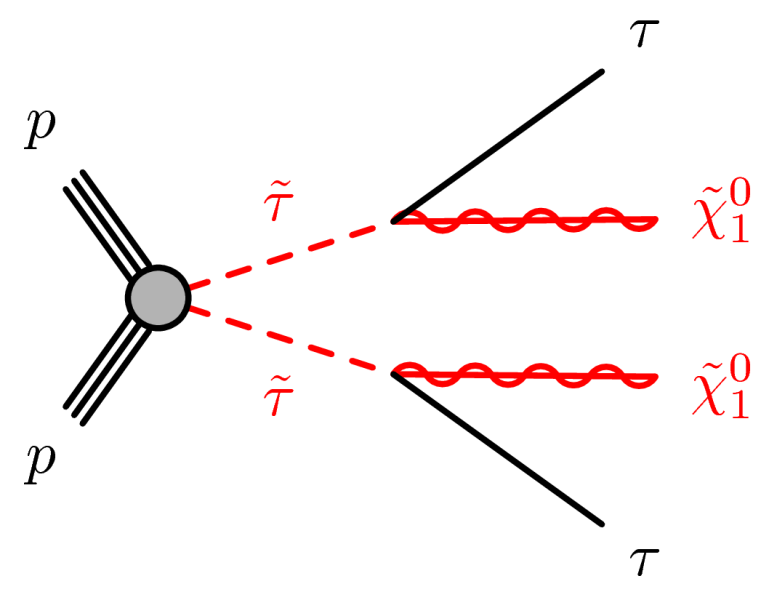
\includegraphics[width=0.4\linewidth]{figs/staustau-tautauN1N1}
 \caption{Diagram for the direct stau pair production followed by each $\tilde{\tau}$ decaying to a $\tau$ lepton and $\tilde{\chi}_1^0$.}
 \label{fig:staustau-tautaun1n1}
\end{figure}

Until recently, the most sensitive searches for direct $\tilde{\tau}$ pair production were performed at the CERN LEP collider~\cite{lep:stau}. As shown in Figure~\ref{fig:lepstau}, LEP limits were set up to stau masses of about 90~GeV, while none of the LHC experiments had sensitivity at higher stau mass regimes.
\begin{figure}[htbp]
 \centering
 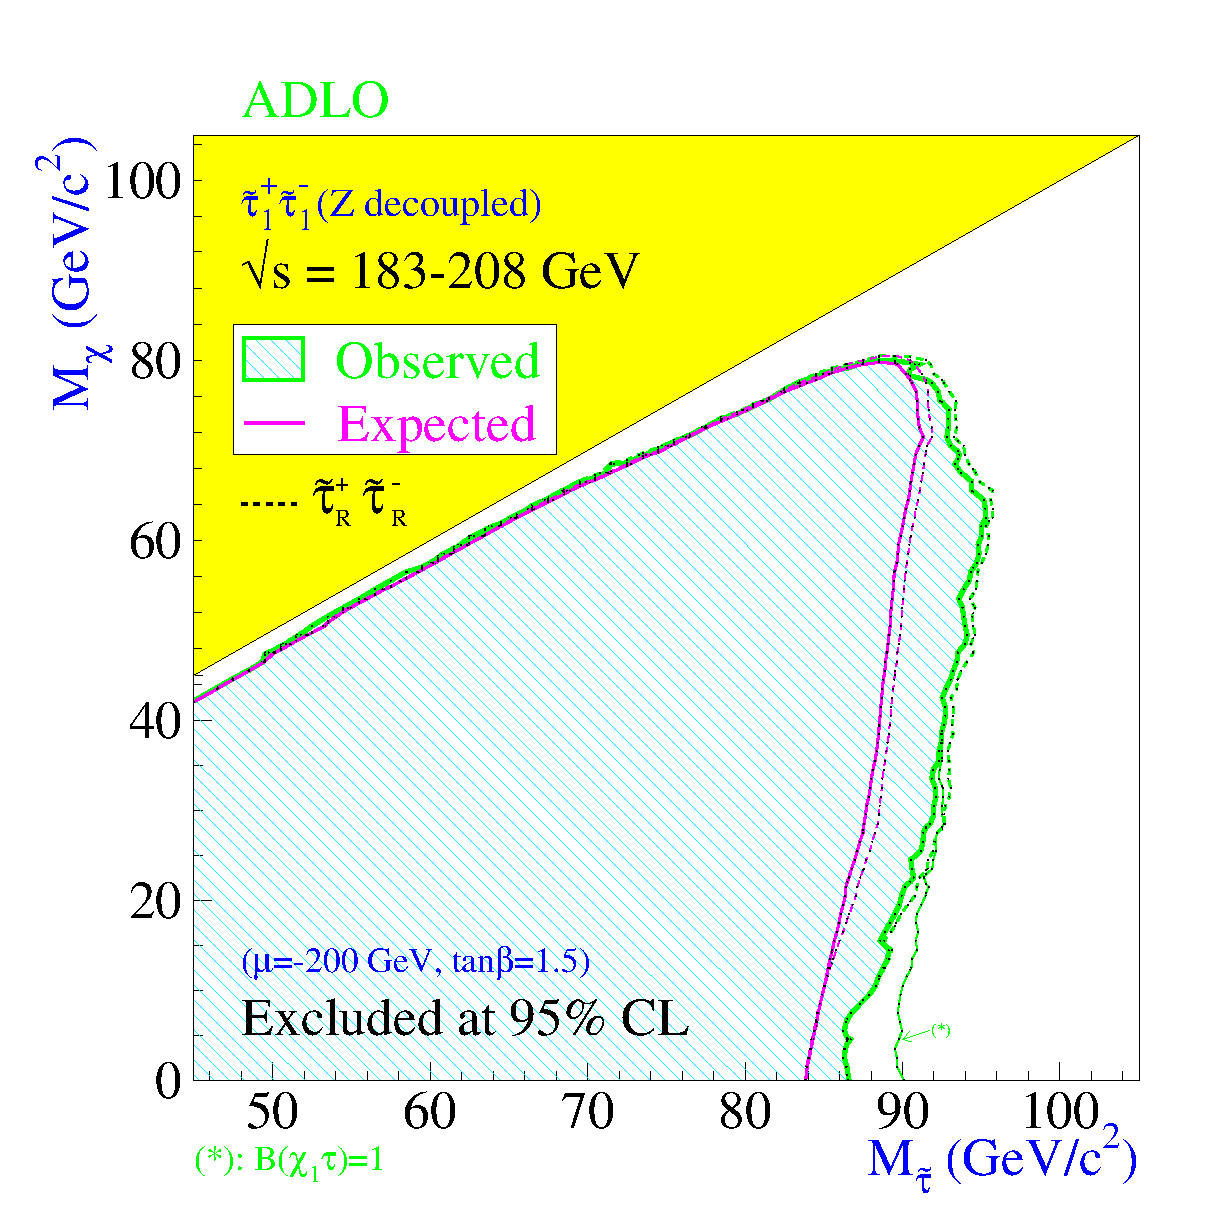
\includegraphics[width=0.7\linewidth]{figs/lep_stau}
 \caption{Expected and observed exclusion limits in the \textit{stau mass - neutralino mass} plane. The branching ratio for right-handed stau decaying to tau lepton + $\tilde{\chi}_1^0$ is included. The results were obtained by combining LEP data collected at center-of-mass energies ranging from 183 GeV to 208 GeV~\cite{lep:stau}.
Stau particles have to be searched for beyond the exclusion limit of around 90~GeV found at the LHC's predecessor at CERN, the Large Electron-Positron collider. 
A light stau, if it exists, could play a fundamental role in neutralino coannihilation, moderating the amount of Dark Matter in the visible universe, which would otherwise
be too abundant to explain the astrophysical measurements.}
 \label{fig:lepstau}
\end{figure}

At the CERN LHC, 
the ATLAS~\cite{Aad:2014yka, Aad:2015eda} and 
CMS~\cite{Khachatryan:2016trj, Khachatryan:2015kxa, Sirunyan:2018vig}
collaborations have both performed searches for direct and indirect stau production with 8 TeV and 13 TeV center-of-mass energy LHC data.  
At 8 TeV center-of-mass energy, ATLAS had no sensitivity to the direct stau-pair production due to the very low low cross-section of the process.
At 13 TeV center-of-mass energy, the CMS collaboration has reported for a degenerate production scenario, in which both left- and right-handed $\tilde{\tau}$ pairs are produced, exclusions of $\tilde{\tau}$ masses up to 150 GeV when assuming a nearly massless neutralino~\cite{CMS:2019eln}.
The ATLAS collaboration has shown results of a search for SUSY in final states with $\tau$ leptons, probing indirect $\tilde{\tau}$ production in models of chargino-neutralino and chargino pair production, using data collected at $\sqrt{s} = 13$~TeV~\cite{Aaboud:2017nhr}. Finally, ATLAS  released in 2019 results of the indirect stau search analysis showing the  first results on upper limits on the $\tilde{\tau}$ production cross-section excluding stau masses from 120~GeV to 390~GeV and a massless lightest neutralino~\cite{ATLAS:2019gti}. 

The search for stau-pairs is very challenging predominantly due to the low production cross section as an electroweak process in hadron collisions (see Figure~\ref{fig:xsec1}). Despite this fact, complex cut-and-count and machine learning techniques are developed to maximize the  sensitivity for scenarios involving the direct production of stau pairs, as well as their indirect production via the decays of charginos and neutralinos.  In this thesis, simplified SUSY models~\cite{PhysRevD.79.075020, PhysRevD.79.015005, Alves_2012} are examined, in which the $\tilde{\tau}$ can be produced directly through pair production, as shown in Figure~\ref{fig:staustau-tautaun1n1}.
The lightest neutralino is the LSP and purely bino, and the two charged staus are assumed to be mass-degenerated. The left- and right-handed staus are assumed to decay with a 100\% branching fraction to a bino-like neutralino, $\tilde{\tau}^\pm_{\mathrm{L},\;\mathrm{R}}  \to \tau^\pm\; \tilde{\chi}_1^0$, whereas all sparticles other than those explicitly mentioned here are assumed to be inaccessible at the LHC energy.
%Furthermore, the search considers final states with two hadronically decaying tau leptons stemming from the $\tilde{\tau}$-pair  decay to two  $\tau$ leptons and two $\tilde{\chi}_1^0$.


\subsection{Methodology}\label{ref:method-stau}

This first ATLAS stau search with LHC Run2 data targets the direct production of a pair of staus, each decaying into one tau lepton and one invisible LSP. Each tau lepton stemming from the $\tilde{\tau}$ decay undergoes a subsequent decay into hadrons ($\tau \to \text{hadrons}\,\, \nu_\tau$) and an invisible neutrino. Signal events would thus be characterized by the presence of two sets of close-by hadrons and substantial missing transverse energy.
The presence of missing transverse energy, which can originate from escaping stable neutralinos as well as neutrinos from tau lepton decays, provides an important source
of discriminating power between signal and background events.
The event classification strongly depends on the amount of missing transverse energy subsequent as well as on the decay mode of the tau lepton stemming from the stau decay. The possible search channels are therefore:
\begin{itemize}
	\item fully-leptonic channel -- both tau lepton leptons undergo weak decays to either electrons or muons, and the associated neutrinos ($\text{BR}\simeq 13\%$);
	\item fully-hadronic channel -- both tau leptons decay weakly to hadrons ($\text{BR}\simeq 42\%$);
	\item lepton-hadron channel -- one tau decays leptonically and the other hadronically ($\text{BR}\simeq 45\%$).
\end{itemize}
The ATLAS analysis explores only the fully-handronic and lepton-hadron channel, with first results being officially released only for the former accounting to approximately the 42\% of the stau events.

\begin{figure}[htbp]
	\centering
	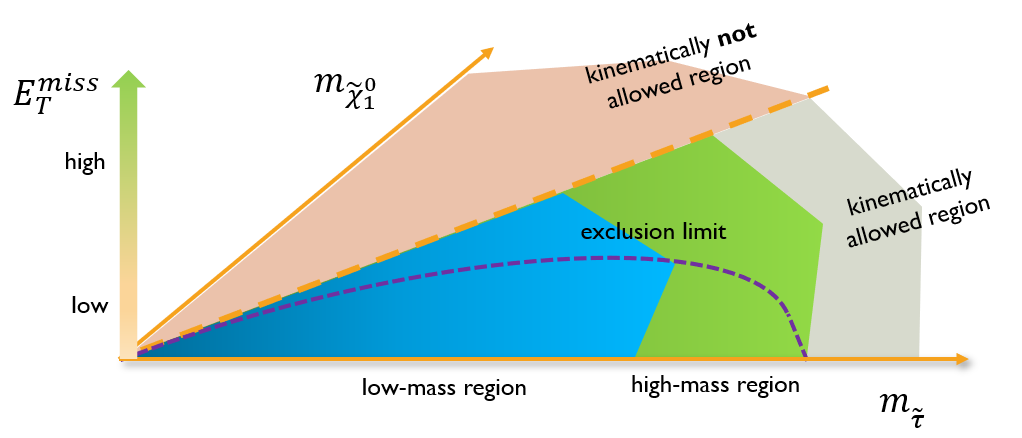
\includegraphics[width=0.8\linewidth]{figs/stau-strat}
	\caption{The analysis exploits the missing transverse energy, $E_\mathrm{T}^\text{miss}$, and stransverse mass observable, $m_{T2}$, to optimize the sensitivity to staus. The search is divided into signal regions with low or high $E_\mathrm{T}^\text{miss}$, targeting therefore scenarios with low or high stau mass.}
	\label{fig:stau-strat}
\end{figure}
The analysis predominantly exploits the missing transverse energy, $E_\mathrm{T}^\text{miss}$, to better optimize the sensitivity to staus (Figure~\ref{fig:stau-strat}).
Orthogonal signal regions (SR) are optimized for stau discovery by varying the kinematic selection criteria, including the particle transverse momentum, $\pt$,
 and the stransverse mass, $m_{T2}$, observable. More specifically, the analysis defines two signal regions,  SR-lowMass  and SR-highMass. The former targets low-mass stau-pair events with missing transverse energy in the window $75-150$~GeV, while the latter selects high-mass stau-pair events with $E_T^\mathrm{miss}>150$~GeV.
Events are required to have have exactly two tau candidates with opposite-sign electric charge (OS). 
They are selected by the asymmetric di-tau trigger to cover the low stau mass region ($75~\text{GeV}<E_\mathrm{T}^\mathrm{miss}<150$~GeV) and by the 
di-tau +$E_\mathrm{T}^\mathrm{miss}$ trigger to cover the high stau mass region ($E_\mathrm{T}^\mathrm{miss}>150$~GeV).


\subsection{Backgrounds}
The main background contributing to the selected final states are SM processes from QCD multijet, W+jets and diboson production.
Background events may contain a combination of `real' tau leptons, defined as correctly identified prompt
tau leptons, or `fake' tau leptons, which can originate from a misidentified quark or gluon jet, an electron, or a muon.  Smaller SM backgrounds arise from Z+jets production, or events that
contain a top quark or a top-quark pair in association with jets or additional W or Z bosons.
To estimate these irreducible background contributions,  MC simulated samples are used and validated in dedicated validation regions. Other SM backgrounds are found to be negligible.

One of the dominant backgrounds in the SRs originates from jets misidentified as tau leptons in multijet
production, where  nearly all hadronically decaying tau candidates are misidentified jets.
The multijet contribution in the SRs is estimated from data using the so-called ABCD method. 
This method defines various non-overlapping regions in a two-dimensional plane, as a function of two (or more) discriminating variables that are largely uncorrelated. More specifically, events are classified in regions differing by the product of electric charge of the tau-pair and the identification requirements of the tau candidates, either loose or tight. These regions are also constructing for varying cuts on the discriminating observables $E_\mathrm{T}^\mathrm{miss}$ or $m_{\mathrm{T}2}$ (see definition in Equation~\ref{eq:mt2}). The number of multijet events in the search region with OS tau-lepton pairs can therefore be calculated from  multijet events in regions identified with tau-lepton pairs having same sign of electric charge (SS) and passing the tight requirements of the tau identification. 
Afterwards, a transfer factor, which is extracted in regions where the tau candidates pass only the loose identification requirements, is used to provide the correct normalization of the multijet estimate.
This transfer factor is defined as the ratio between the number of events with OS tau pairs to the number of events with SS tau-pair candidates.


The multijet background estimation is also validated using a different method, the \textit{fake-factor} method. Fake factors (FF) are derived for each of the two tau candidates with the same electric charge in a multijet enriched region. They are computed as the ratio of the number of leading or subleading tau candidates passing all of the nominal signal identification criteria over the number of tau candidates failing the requirement on the tau identification, and are parameterized with respect to the $p_T$, $\eta$ and number of tracks of the tau candidates. The expected number of multijet events entering a selection is computed by applying the fake factors to the yields in a set of sideband regions where either the leading, subleading or both tau candidates fail the identification requirements. Agreement of the predicted multijet event yields from the ABCD method and the FF method is observed within the statistical and systematic uncertainties.


The production of W+jets events with at least one misidentified tau lepton is an important background,
accounting for about 25\% of the expected SM background in the two SRs. It is  estimated from MC simulation and normalized to data in a dedicated control region.

\subsection{Systematic uncertainties}
Systematic uncertainties have an impact on the estimates of the background and signal event yields in the signal regions. 
Uncertainties arising from experimental and theoretical sources are estimated in the analysis and considered in the statistical analysis to interpret the results. 
The main sources of experimental systematic uncertainty in the SM background estimates include tau lepton and jet energy scale and resolution, tau lepton identification, pile-up, and uncertainties related to the
modelling of $E_\mathrm{T}^\text{miss}$ in the simulation. 
Uncertainties arising from ABCD method to determine the QCD multijet events are also considered, dominated by the the correlation between the tau identification, the charge requirement, and the kinematic variable $m_{\mathrm{T}2}$.
Finally, theoretical uncertainties affecting the MC event generator predictions, for the W+jets, Z+jets
and multi-boson samples, are estimated by varying the renormalization and factorization scale as well as
PDF uncertainties. The dominant uncertainties in the SRs are tau identification and energy scale (14 - 29\%) and the statistical uncertainty of the signal MC predictions (6 - 10\%). 
The multijet normalization with respect to the prediction from the ABCD method in the SR has an uncertainty
of around 30\%, due to the small number of observed events in the multijet regions.
The cross-section uncertainty is taken into account as main source of signal modelling theoretical uncertainty, and it varies from 3\% to 7\% for the considered SUSY models.


\subsection{Results}

Selected events are distributed according to the $m_{\mathrm{T}2}$ observable for data, expected SM backgrounds, and the SUSY signal models.  In both signal regions of the analysis, SR-lowMass and SR-highMass, observations and background predictions are found to be compatible within uncertainties.
The $m_{T2}$ distributions are shown in Figure~\ref{fig:stau-distr} for data, expected SM backgrounds, and two SUSY scenarios with different stau masses. 
In both signal regions, observations and background predictions are found to be compatible within uncertainties.
\begin{figure}[h]
	\centering
	\begin{subfigure}[b]{0.7\textwidth}
		\includegraphics[width=\textwidth]{figs/mt2-1.png}\caption{SR-lowMass }	\label{fig:mt2-2}
	\end{subfigure}
	~ 
	\begin{subfigure}[b]{0.7\textwidth}
		\includegraphics[width=\textwidth]{figs/mt2-1.png} \caption{SR-highMass }	
		\label{fig:mt2-2}
	\end{subfigure}
	\caption{	The post-fit $m_{T2}$ distribution for SR-lowMass (\ref{fig:mt2-2}) and SR-highMass (\ref{fig:mt2-2}). 
		The stacked histograms show the expected SM backgrounds.
		The hatched bands represent the sum in quadrature of systematic and statistical uncertainties of the total SM background. 
		For illustration, the distributions from SUSY reference points differing by stau mass are also shown as dashed lines. 
		The last bin includes the overflow events. Adapted from Ref.~\cite{ATLAS:2019gti}. }\label{fig:stau-distr}
\end{figure}

In the absence of a significant excess over the expected SM background, the observed and expected numbers
of events in the signal regions are used to place exclusion limits at 95\% CL using the model-dependent limit fit. The exclusion limits for the combined low-mass and high-mass SRs for the simplified models described previously are shown in Figure~\ref{fig:stau-limits-atlas}.
While the left-handed stau pair production has a higher production cross section, the right-handed stau pair production has a higher efficiency times acceptance due to kinematic differences in the resulting decay products. Stau masses from 120 GeV to 390 GeV are excluded for a massless lightest neutralino in the scenario of the combined left- and right-handed stau-pair production.
These limits significantly extend previous results~\cite{Aad:2015eda, Khachatryan:2014qwa, Sirunyan:2018vig} in the high $\tilde{\tau}$ mass region.
The exclusion limits from the stau analysis can be compared to other SUSY electroweak searches involving two light charged leptons ($\ell=e,\,\mu$) in the final state. Figure~\ref{fig:atlas-ml} shows the exclusion limits at 95\% CL for the $2\ell$ compressed, $2\ell$, $2\tau$ and results from LHC with $\sqrt{s}=8$~TeV data and LEP.
The exclusion limits are shown in the plane of the lightest supersymmetric neutralino $\tilde{\chi}_1^0$ and the invariant mass of the produced and decaying slepton.

\begin{figure}[h]
	\centering
	\begin{subfigure}[b]{0.7\textwidth}
		\includegraphics[width=\textwidth]{figs/stau-limits-atlas.png}\caption{Stau exlcusion limits}\label{fig:stau-limits-atlas}
	\end{subfigure}
	~ 
	\begin{subfigure}[b]{0.7\textwidth}
		\includegraphics[width=\textwidth]{figs/atlas-ml} \caption{Slepton exlcusion limits}\label{fig:atlas-ml}	
	\end{subfigure}
	\caption{Plot~\ref{fig:stau-limits-atlas}: The 95\% CL exclusion contours for the combined fit of low-mass and high-mass signal regions for simplified models with combined production. The solid (dashed) lines show the observed (expected) exclusion contours. The band around the expected limit shows the $\pm 1~\sigma$ variations, including all uncertainties except theoretical uncertainties in the signal cross section. The dotted lines around the observed limit indicate  the sensitivity to $\pm 1~\sigma$ variations of the theoretical uncertainties in the signal cross section~\cite{ATLAS-CONF-2019-018, ATLAS:2019gti}. 
		%
	Plot~\ref{fig:atlas-ml}: Exclusion limits at 95\% CL based on 13 TeV data in the (slepton, lightest neutralino) mass plane for different analyses probing the direct production of sleptons with decays to lepton neutralino. The types of sleptons (flavor and coupling) included in each search is specified in the legend~\cite{ATL-PHYS-PUB-2019-022}.	
}\label{fig:stau-results}
\end{figure}



\subsection{Comparison with CMS}

In Ref.~\cite{CMS:2019hos}, CMS presents a search for direct tau slepton pair production using data from proton-proton collisions at a center-of-mass energy of 13 TeV. Events are selected by requiring a tau lepton pair and significant missing transverse momentum. 
CMS defines search regions using various kinematic observables that exploit expected differences in discriminants between signal and background. 
The data used for this search correspond to an integrated luminosity of $77.2~\mathrm{fb}^{-1}$ collected in 2016 and 2017, which amount about the half of the data that ATLAS uses for the respective analysis.

CMS observes no excess above the expected SM background and thus sets upper limits on the cross section for direct stau pair production for simplified models,
in which each $\tilde{\tau}$ decays to a tau lepton and the lightest neutralino, with the latter being assumed to be the lightest supersymmetric particle (Figure~\ref{fig:CMS-SUS-18-006-stau}). 
Assuming a mass-degenerate stau production model, in which both left- and right-handed helicity stau pairs are produced, CMS excludes stau masses up to 150 GeV, 
under the assumption of a nearly massless neutralino.
\begin{figure}
	\centering
	\includegraphics[width=0.8\linewidth]{figs/CMS-SUS-18-006-stau.png}
	\caption{Upper limit on the cross section of stau-pair production excluded at 95\% CL as a function of the stau mass in degenerate stau models 
		for a $\tilde{\chi}_1^0$ mass of 1~GeV. 
		The results shown are for the statistical combination of the 2016 and 2017 CMS data in the lepton-hadron and hadron-hadron ditau final states~\cite{CMS:2019hos}.}\label{fig:CMS-SUS-18-006-stau}
\end{figure}


Compared to the ATLAS analysis, CMS considers both the hadronic and leptonic decay modes of the tau lepton. 
In the additional lepton-hadron ditau channel, one tau can decay to one or more hadrons and a neutrino,
and the other to an electron or muon and two neutrinos.
Moreover, CMS uses dedicated machine learning techniques to enhance the search sensitivity. 
These include the incorporation of an improved hadronic tau selection method that makes use of a deep neural network for the fully-hadronic ditau analysis, 
and of a boosted decision tree (BDT) for event selection in the lepton-hadron analyses. 

\subsection{Conclusions}
Searches for the direct production of light stau pairs at the hadron colliders are motivated by both experimental
and theoretical considerations. Being an electroweak process, the stau production at LHC has a lower cross-section compared to SUSY processes involving the 
production of sparticles via strong interactions. In addition, hadronically decaying taus can be easily mimicked QCD jets and electrons making thus the tau reconstruction and identification more challenging.

Prior to the Run2 ATLAS analysis, the most stringent exclusion limits are from LEP, 
making the search for direct staus crucial in the hunt for SUSY at the LHC. 
Staus are expected to be the lightest slepton flavor in models of GUT scale unification and the lighter stau is favoured to be
mostly right-handed. Furthermore, in models with a light stau and lightest neutralino $\tilde{\chi}_1^0$ 
with a small mass difference, stau co-annihilation processes in the early universe can reduce the $\tilde{\chi}_1^0$ relic density
and make it consistent with observations from cosmological measurements.

Searches for stau-pair production in events with at least two hadronically decaying $\tau$-leptons and missing
transverse momentum were performed using $139~\mathrm{fb}^{-1}$ of $pp$ collision data at $\sqrt{s} = 13$~TeV recorded with
the ATLAS detector at the LHC~\cite{ATLAS-CONF-2019-018, ATLAS:2019gti}.
Search regions are defined using kinematic observables that exploit expected differences in discriminants between signal and background.
Agreement between data and SM predictions is observed in all optimized signal regions. 
The results are, therefore, used to set upper limits on the visible cross section for events beyond the SM in each signal region.
Exclusion limits are placed on parameters of simplified electroweak supersymmetry models in scenarios of stau-pair production. 
Stau masses from 120 GeV to 390 GeV are excluded for a massless lightest neutralino in the scenario of direct production of stau pairs, with each stau decaying into the lightest neutralino $\tilde{\chi}_1^0$ and one $\tau$-lepton. 
These limits extend significantly beyond previous results by the ATLAS and CMS experiments in the high stau mass region.

%=============================================================================================================================

\chapter{Synopsis}

\section{Summary}

The search of SUSY is an important part of the physics program at CERN's LHC. The large amount of data successfully collected by the experiments so far, provide a unique opportunity to explore SUSY with novel analysis techniques.

If particles predicted by SUSY exist and are not extremely massive, they must be produced at LHC collision events and could be hiding in data collected by the ATLAS and CMS detectors. However, unlike most processes at the LHC, which are governed by strong force interactions, electroweak superpartners would be created through the much weaker electroweak interaction, thus lowering their production rates. Further, most of these new SUSY particles are expected to be unstable and can be searched by tracing their decay products -- typically into a known  SM particle and a \textit{LSP}, which could be stable and non-interacting, thus forming a natural dark matter candidate. 

Despite the low production cross-section of electroweak SUSY processes, events with many leptons in the final state are very interesting since SM processes mimicking them are very rare.
ATLAS searched for such multi-lepton events and presented the results in terms of the number of events from new physics processes with a four-lepton signature, and also in terms of RPV and RPC SUSY models.  All data yields are found to be consistent with  SM expectations and results are thus used to set upper limits on the event yields from processes beyond the   SM. 
Stringent exclusion limits are set in simplified models of
GGM SUSY with higgsino particles, which are assumed to decay into either Higgs or Z bosons.  In RPV simplified models with decays of the LSP to charged leptons, exclusions are placed on the mass of wino, slepton and gluino masses up to the TeV scale, extending significantly the lower limit results set by previous ATLAS searches.
 

Until recently, an important superpartner of the tau slepton, the "stau", had yet to be searched for beyond the exclusion limit of around 90 GeV found at the LHC's predecessor at CERN, the LEP collider. 
A light stau, if it exists, could play a role in neutralino co-annihilation, moderating the amount of dark matter in the visible universe, which otherwise would be too abundant to explain astrophysical measurements. The search for a light stau is experimentally challenging due to its extremely low production rate in LHC $pp$ collisions, requiring advanced techniques to reconstruct the  SM tau leptons it can decay into. In fact, during the LHC Run 1 data taking period, only a narrow parameter region around a stau mass of 109 GeV and a massless lightest neutralino could be excluded by LHC experiments~\cite{Aad:2015eda}. 
In LHC Run 2, ATLAS search efforts target the direct production of a pair of staus, each decaying into one tau lepton and one invisible LSP.  The ATLAS data do not reveal hints for stau pair production and thus new exclusion limits are set on the mass of staus using different assumptions on the presence of both possible stau types (left and right, referring to the two different spin states of the tau partner lepton). The limits obtained supersede significantly the LEP results and are in fact the strongest obtained so far in collider experiments.

Overall, both sets of results place strong constraints on important supersymmetric scenarios, which will guide future ATLAS searches. Further, they illustrate the benefits brought by advanced analysis techniques, which help improve the sensitivity to new physics phenomena at colliders in the future.

%=============================================================================================================================
\section{Prospects}

\subsection{Ditau Reconstruction for Four-lepton Searches}

Due to the low SM background, the search for four-lepton final states provides excellent sensitivity to R-parity violating SUSY models,
where the LSP, produced in pairs, decays into final states with at least two charged leptons. 
For LSP decays into hadronically decaying $\tau$ lepton pairs, however, the current analysis is not sensitive if the mass difference between LSP and the next heavier NLSP is large. This is because the $\tau$ jets become highly collimated and the standard $\tau$ reconstruction algorithm is not able to resolve them. An example of collimated hadronic di-tau decays is shown in Figure~\ref{fig:ditau--dr}, which presents the $\Delta R$ distribution of the the two taus at truth level.
\begin{figure}
	\centering
	\includegraphics[width=0.7\linewidth]{figs/ditau--dr}
	\caption{$\Delta R$ distribution between the the members of the tau-pair, as measured in RPV gluino events of diagram~\ref{fig:fig_01d}. 
		The standard reconstruction fails for $\Delta R <  0.4$, as the overlap between the two tau jet cones is very high.}
	\label{fig:ditau--dr}
	\end{figure}
As a consequence, the sensitivity for low $\tilde{\chi}_1^0$ masses is significantly lowered, as it can be seen in Figure~\ref{fig:excl-gluino}.

A new specialized high-$\pt$ $\tau$ jet pair reconstruction method has been developed, in parallel to the four-lepton SUSY analysis, that exploits the LHC Run-2 
dataset at 13 TeV center-of-mass energy~\cite{rendel-ditau}. The di-tau reconstruction uses jets with a large distance parameter $\Delta R = 1.0$ and attempts to reconstruct two hadronically decaying taus into a single jet. It requires a minimum $\pt$ of 50~GeV for the di-tau object within the barrel region of the detector, $|\eta|<2.5$.
At least two subjects with $R=0.2$ with minimum one associated track is required in order to avoid picking up objects which are not hadronically decaying taus.
To further improve the performance of the ditau reconstruction, 
a BDT algorithm is trained using tracking and calorimeter information associated to the subjets. As signal objects, truth-matched tau-lepton pairs from SUSY RPV gluino processes are used, trained against di-tau candidates from QCD jet data, $t\bar t$ and $Z \to e^+ e^-$+jets (Figure~\ref{fig:ditau-bdt}).
\begin{figure}
	\centering
	\includegraphics[width=0.7\linewidth]{figs/ditau-bdt}
	\caption{Di-tau BDT score distributions for signal (blue) and background (red) di-tau objects.}
	\label{fig:ditau-bdt}
\end{figure}
By selecting reconstructed di-tau candidates with a minimum BDT score at 0.5, the di-tau algorithm achieves a flat identification efficiency of 60\% 
for ditau objects with $\pt > 150$~GeV containing subjets with distance $0.2 < \Delta R < 0.4$, i.e. in the proximity zone where the standard ATLAS tau reconstruction fails to reconstruct any tau candidate. 

Finally, the results of the di-tau reconstruction algorithm are tested in an RPV gluino scenario with $m_{\tilde{g}}=1500$~GeV and $m_{\tilde{\chi}_1^0}=50$~GeV, where the sensitivity of the current SUSY four-lepton search is very limited. A significant improvement in the sensitivity is observed for a signal region region defined with two light charged leptons and a least one reconstructed di-tau, as shown in Figure~\ref{fig:di-tau-results}.

\begin{figure}[hp]
	\centering
	\begin{subfigure}[b]{0.75\textwidth}
		\includegraphics[width=\textwidth]{figs/ditau-meff}
	\end{subfigure}
	~ 
	\begin{subfigure}[b]{0.75\textwidth}
		\includegraphics[width=\textwidth]{figs/ditau-sens}
		\label{fig:fig_07b}
	\end{subfigure}
	\caption{Top: distribution of the $m_\text{eff}$ observable in a signal region with two charged light leptons and a hadronic di-tau candidate with $\pt>150$~GeV and  BDT score greater than 0.5. The results are shown for an RPV gluino model with  $m_{\tilde{g}}=1500$~GeV and $m_{\tilde{\chi}_1^0}=50$~GeV.
	Bottom: expected sensitivity contours for the same SUSY model and signal region. With the $m_\text{eff}>1500$~GeV requirement, the di-tau method helps to increase the  sensitivity in the low LSP mass range. }\label{fig:di-tau-results}
\end{figure}

The di-tau algorithm shows very promising capabilities by recovering low-$\pt$ tau pairs, which are otherwise lost when using the current tau reconstruction of ATLAS.
This technique is currently integrated in the entire SUSY four-lepton analysis.

\subsection{Multivariate Analysis for Stau Searches}
As discussed in Section~\ref{ref:method-stau}, the lepton-hadron final state decay of the tau pair has a branching ratio of 45\%, resulting thus to a significant fraction of stau events decaying to taus. Carrying out an analysis targeting the lepton-hadron ($\tau_\ell \tau_h$) final states with one tau decaying hadronically and the other to either an electron or muon, is expected to bring additional sensitivity to the current search of staus with two hadronic taus only ($\tau_h \tau_h$) .

As in the case of the fully-hadronic ditau channel, the presence of missing transverse momentum  can originate 
from stable neutralinos as well as neutrinos from $\tau$ lepton decays, providing thus an important source of discriminating power between signal and background.
Although the search strategy in the $\tau_h \tau_h$ final state can rely on a cut-and-count-based analysis to reject backgrounds and select signal events, 
it is definitely not going to be sufficient for the $\tau_\ell \tau_h$ final states. 
The reason behind this, is the overwhelming $W\to\ell\nu+$jets SM process which makes it the dominant background for the $\tau_\ell \tau_h$ search.
W bosons can decay into a charged light lepton and neutrino with the emission of QCD jets that can confuse the reconstruction and identification of hadronically decaying taus. Therefore, more advanced analysis techniques must be deployed in order to efficiently reject backgrounds and select as much signal events as possible.

\begin{figure}
	\centering
	\includegraphics[width=0.6\linewidth]{figs/Wlnu}
	\caption{Feynman diagram for the main background process of the lepton-hadron ditau final state. The outgoing quark from the $W\to\ell\nu$ process can lead to a jet that can fake a hadronically decaying tau.}
	\label{fig:wlnu}
\end{figure}


To achieve the desired discrimination between signal and background, 
a multivariate analysis was developed in parallel to the efforts of the ATLAS stau analysis with two hadronically decaying taus (Figure~\ref{fig:stau-training}).
The data used in this search are selected through triggers that require the presence of isolated electrons and muons.
For the $\tau_\mu \tau_h$ final state, the trigger is based on the presence of an isolated muon with $\pT > 20$~GeV in 2015, $\pT > 24$~GeV in early 2016 and $\pT > 26$~GeV for the rest of the data taking period. For electrons, a combination of triggers with $\pt>24,\,26,\, 60,\, 140$~GeV is used across the entire 2015-2018 dataset.

The $\tau_\ell \tau_h$ search initially analyzes the $\tau_e \tau_h$ and $\tau_\mu \tau_h$ channels separately and combines them statistically in a combined maximum-likelihood fit afterwards. To better optimize the sensitivity of the search, the events are split into two big categories according to the presence of a high-$\pt$ jet in the event or not: 0-jet and 1-jet signal regions. While $W\to\ell\nu+$jets is a dominant background in the lepton-hadron channels, the
relative contributions from other backgrounds from top-quark, $Z\to \ell\ell$ and other vector-boson decays, as well as
from misidentified leptonic or hadronic $\tau$ decays, contribute considerably. Therefore, dedicated control regions are developed to understand the physics modelling of each of these background processes compared to real data. During the statistical fit, each of the  normalization of the $W+$jets, top-quark and the Drell-Yan $Z\to \ell \ell$+jets backgrounds is constrained via adjacent control regions which are depleted of these background processes. A summary of the statistical model is diagrammatically shown in Figure~\ref{fig:lh-strat}.

\begin{figure}[htbp]
	\centering
	\includegraphics[width=0.9\linewidth]{figs/lh-strat}
	\caption{Summary of the lepton-hadron statistical model. 
		The stau final states are categorized according to the leptonic decay of one of the taus: electron-hadron and muon-hadron channels.
		The analysis is performed separately in each channel using different observables and selection cuts in order to mitigate the different composition of background events. The events in each channel are split into 0-jet and 1-jet based on the presence of a high-$\pt$ in the event. 
		The results from the electron-hadron and the muon-hadron channels are statistically combined in a combined maximum-likelihood fit. 
		The main backgrounds are constrained via a normalization factor which is connected to adjacent control regions which are rich for each of these backgrounds.
		All experimental and theoretical uncertainties count for nuisance parameters in the fit.}
	\label{fig:lh-strat}
\end{figure}


In view of the signal-to-background conditions, and in order to exploit correlations between final-state observables, 
a multivariate analysis technique, based on boosted decision trees (BDTs), is used to extract the final results.
Boosted decision trees are used in each category, 0-jet and 1-jet, to extract the stau signal from the large number of background events. 
Decision trees recursively partition the parameter space into multiple regions where signal or background purities are enhanced. 
Boosting is a method which improves the performance and stability of decision trees and involves the combination of many trees into a single final discriminant. 
After boosting, the final score undergoes a transformation to map the scores in the bin range 0-9.
The most signal-like events have high BDT scores,  while the most background-like events accumulate on the left-hand side of the BDT score distribution.
Separate BDTs are trained for each decay channel with the corresponding signal and background samples.
The separate training naturally exploits differences in event kinematics between different stau production modes.
It also allows different discriminating variables to be used to address the different background compositions in each channel.

A large set of potential variables was investigated, in each channel separately, and only those variables which led to an improved discrimination
performance of the BDT were kept. The most discriminating variables are found the be the pseudorapidity distance between the light charged lepton and the tau $\Delta \eta(\ell,\, \tau_h)$, the significance of the missing transverse energy  $S_{E_T^\text{miss}}$, the transverse mass defined with the lepton $m_T(\ell) = \sqrt{2 E_T^\text{miss} p_T^{\ell}(1-\cos\theta)}$ (where $\theta$  is the angle between the $E_T^\text{miss}$ and the lepton in the transverse plane), the tau $\pt$ and the BDT score of the tau candidate against QCD jets.

\begin{figure}[tbhp]
	\centering
	\begin{subfigure}{0.7\textwidth}
		\includegraphics[width=\textwidth]{figs/bdt-wip.png}
		\caption{BDT scores}
		\label{fig:bdt-up}
	\end{subfigure}
	~ 
	\begin{subfigure}{0.7\textwidth}
		\includegraphics[width=\textwidth]{figs/roc-wip.png}
		\caption{ROC curves}
		\label{fig:roc-down}
	\end{subfigure}
	\caption{Distribution of the BDT classifier scores (\ref{fig:bdt-up}) and the corresponding ROC curve (\ref{fig:roc-down}) for a BDT algorithm trained in
		0-jet category of the electron-hadron channel. A perfect classification would correspond to a rectangular ROC curve, while a completely random classification, namely a random selection of background and signal events, would correspond to a straight diagonal line. To describe the training quality, the area under the ROC curve (ROC-AUC) is used.
		The ROC curves in the training and testing datasets are shown for the nominal (solid line) and for the cross-validation (dashed lines) training sessions.
		The number in brackets indicate the ROC-AUC.
		The distribution of events (\ref{fig:bdt-up}) from the training sample for background and signal processes are shown as blue and red hatched areas, respectively.
		The test samples are shown as data points. The $\chi^2$ test serves as a similarity test between the training and testing datasets during the BDT training session and helps to control possible overfitting effects. 
	}\label{fig:stau-training}
\end{figure}



After training the classification algorithm, the BDT output in the two analysis categories provides the final discrimination. Figure~\ref{fig:stau-bdt} shows the distribution of the BDT output for signal and background events, as well as for data.
The BDT score distributions for signal and background events are used to build a statistical model for each channel and category.
A maximum-likelihood fit is performed on all categories simultaneously assuming Asimov statistics, i.e. the observed data are set to the total measured background.
The signal strength, $\mu$, defined as the ratio of the measured signal yield to the Standard Model expectation is conditionally set to 1, allowing to measure the
expected significance of the search.
The statistical analysis of the data employs a binned likelihood function $L(\mu,\, \vec{\theta})$, 
constructed as the product of Poisson probability terms.
The impact of systematic uncertainties on the signal and background expectations is
described by nuisance parameters, $\vec{\theta}$, 
which are each parameterized by a Gaussian or log-normal constraint. 
The expected numbers of signal and background events in each bin are functions of $\vec{\theta}$. 
The test statistic $q_\mu$ is then constructed according to the profile likelihood ratio:
$$q_\mu = - 2 \ln \frac{L(\mu,\, \hat{\hat{\vec{\theta}}})}{L(\hat{\mu},\, \hat{\vec{\theta}})}$$
where $\hat{\mu}$  and  $\hat{\vec{\theta}}$ are the parameters that maximize the likelihood 
and $\hat{\hat{\vec{\theta}}}$ are the nuisance parameter values that maximize the likelihood for a given $\mu$ ($\mu=1$ in the case of an Asimov model).
\begin{figure}
	\centering
	\includegraphics[width=0.8\linewidth]{figs/stau-bdt-wip}
	\caption{Preliminary results on the distributions of the BDT discriminant for signal ($m_{\tilde{\tau}}=200$~GeV and $m_{\tilde{\chi}_1^0}=1$~GeV) and background events in the 0-jet category. 	The post-fit error includes all statistical and statistical uncertainties.
	The W+jets and top-related background events are simultaneously constrained though their normalization factors connected to the respective control regions.
The excess of events, above the background, shown by a solid red area corresponds to stau-pair signal events.  }
	\label{fig:stau-bdt}
\end{figure}
With the Asimov asymptotic testing, the expected significance for the benchmark direct stau scenario with $m_{\tilde{\tau}}=200$~GeV and $m_{\tilde{\chi}_1^0}=1$~GeV is found to be $1.0~\sigma$ including all systematic uncertainties, $2.0~\sigma$ without any uncertainties and $1.6~\sigma$ with all uncertainties but excluding the so-called $\gamma$ statistical factors which parameterize the statistical uncertainty per BDT bin in the statistical model.

Despite the low significance of the lepton-hadron channel alone, it is expected that the statistical combination of the lepton-hadron and hadron-hadron channels together will further extend the analysis sensitivity particularly in the compressed zone (small mass differences between the LSP and the stau masses). 
The hadron-hadron channels is currently insensitive in the compressed area mainly due to the high $\pt$ cuts on the the tau candidates, as the di-tau triggers used by
the analysis have relatively high online $\pt$ thresholds.



\subsection{Stau Searches at HL-LHC}
The search for weak-scale SUSY is one of the highest physics priorities for the current and future LHC runs.
In the Run-2 data-taking period (2015-2018), the ATLAS experiment collected $149~\mathrm{fb}^{-1}$ of proton-proton collisions
from the LHC at centre-of-mass energies of 13 TeV, with an average number of collisions per bunch
crossing of $\langle \mu \rangle = 34$. 
During the second long shutdown (LS2) of the LHC program (2019-2021), 
the injection chain is foreseen to be modified and the accelerator will be able to achieve centre-of-mass-energies of 14 TeV.
During LS3 (2025-2027), the accelerator is foreseen to be upgraded to the high luminosity LHC (HL-LHC), 
which is expected to deliver an integrated luminosity of about $3000~\mathrm{fb}^{-1}$, with an average number of pileup interactions per bunch
crossing of $\langle \mu \rangle = 200$. The large dataset expected at the end of HL-LHC offers an unprecedented discovery potential for heavy SUSY particles in
the electroweak sector, of masses around or above a TeV.

ATLAS has recently studied the physics sensitivity at the end of HL-LHC to direct production of various SUSY partners in the electroweak sector including staus.
Searches for the direct production of light stau pairs at the HL-LHC are motivated by both experimental and theoretical considerations. 
As of today the most stringent exclusion limits exclude stau masses up to 350~GeV assuming a nearly massless LSP, making the
search for direct staus a crucial ``unturned stone" in the hunt for SUSY at the LHC program. 
As discussed in Section~\ref{sec:stau-motivation}, 
staus are expected to be the lightest slepton flavor in models of GUT scale unification and the lighter stau is favoured to be
mostly right-handed. 
Furthermore, in models with a light stau and lightest neutralino $\tilde{\chi}_1^0$ with a small mass difference, 
stau co-annihilation processes in the early universe can reduce the $\tilde{\chi}_1^0$ relic density
and make it consistent with observations from cosmological measurements.

To study the sensitivity to stau-pair production, ATLAS performed a search in which final states with two hadronically decaying
tau leptons are considered. 
Two simplified models describing the direct production of stau-pairs were used: 
one considered stau partners of the left-handed tau lepton ($\tilde{\tau}_L$), 
and a second considers stau partners of the right-handed tau lepton ($\tilde{\tau}_R$). 
In both models, the stau is assumed to decay with a branching fraction of 100\% to the SM tau-lepton and the LSP.

The signature considered is two hadronically decaying taus, low jet activity because of the electroweak nature of the process, 
and large missing transverse momentum from the undetected $\tilde{\chi}_1^0$ and neutrinos. 
Like in the ATLAS analysis with LHC Run2 data, the SM background is dominated by $W/Z+$jets, multi-boson, multi-jet, and top pair production. 
Also, the stransverse mass $m_{T2}$ is used to further discriminate SUSY events from SM processes.
In this analysis, three signal regions are defined to maximize model-independent discovery sensitivity based on the
optimization for scenarios with low (SR-low), medium (SR-med) and high (SR-high) mass differences
between the $\tilde{\tau}$ and $\tilde{\chi}_1^0$. Each SR is identified by the range of the $m_{T2}$ considering both hadronically decaying taus in the event.

\begin{figure}[htb]
	\centering
	\includegraphics[width=0.75\linewidth]{figs/hl-lhc-stau}
	\caption{The 95\% CL exclusion and discovery potential for direct stau production at the HL-LHC ($3000~\mathrm{fb}^{-1}$ at $\sqrt{s} = 14$~TeV), 
		assuming $\tilde{\tau}_L \tilde{\tau}_L$, $\tilde{\tau}_L \tilde{\tau}_R$ and $\tilde{\tau}_R \tilde{\tau}_R$ production~\cite{ATLAS:2018diz}.}
	\label{fig:hl-lhc-stau}
\end{figure}


Figure~\ref{fig:hl-lhc-stau} shows the 95\% CL exclusion limits and discovery potentials calculated 
for  $\tilde{\tau}_L \tilde{\tau}_L$ and $\tilde{\tau}_R \tilde{\tau}_R$ production, either alone or in combination, assuming a massless $\tilde{\chi}_1^0$.
The exclusion limit reaches 730 GeV in stau mass for the combined $\tilde{\tau}_L \tilde{\tau}_L$ and $\tilde{\tau}_R \tilde{\tau}_R$,
and 680 GeV (420 GeV) for pure  $\tilde{\tau}_L \tilde{\tau}_L$ (pure $\tilde{\tau}_R \tilde{\tau}_R$) production with a massless $\tilde{\chi}_1^0$.
The discovery sensitivity reaches 110-530 GeV (110-500 GeV) in stau mass for the combined  $\tilde{\tau}_L \tilde{\tau}_L$ and $\tilde{\tau}_R \tilde{\tau}_R$,
(pure $\tilde{\tau}_L \tilde{\tau}_L$) production with a massless $\tilde{\chi}_1^0$.


Based on the search channels and methods considered in this ATLAS analysis, the HL-LHC is not expected to have discovery
potential for the stau co-annihilation scenario or for the production of light right-handed stau pairs $\tilde{\tau}_R \tilde{\tau}_R$  (as the cross-section is very small), making these scenarios excellent benchmarks for further study at HL-LHC as well as for future collider-based
experiments. 




%=============================================================================================================================

\section{Outlook}

The absence of any observation of new phenomena at the first run of the LHC
at $7,\, 8,\, 13$~TeV place significant constraints on SUSY parameter space. 
As displayed in Figure~\ref{fig:susysum}, inclusive searches probe production of gluinos at about 2.2 TeV, 
first and second generation squarks in the range of about 1 to 1.8 TeV, 
third generation squarks at scales around 600 GeV to 1 TeV,
electroweak gauginos at scales around 300 to 800 GeV, and sleptons up to 800 GeV. 
However, depending on the assumptions made on the underlying SUSY spectrum these limits can also weaken considerably.
\begin{sidewaysfigure}
%\begin{figure}
	\centering
	\includegraphics[width=0.99\linewidth]{figs/susysum}
	\caption{Mass reach of the ATLAS searches for SUSY. Results are quoted for the nominal cross section in both a region of near-maximal mass reach and a demonstrative alternative scenario, in order to display the range in model space of search sensitivity. Some limits depend on additional assumptions on the mass of the intermediate states, as described in the references provided in the plot. In some cases these additional dependencies are indicated by darker bands showing different model parameters~\cite{ATL-PHYS-PUB-2019-022}.}
	\label{fig:susysum}
%\end{figure}
\end{sidewaysfigure}

With the LHC having reached almost its maximum energy of $\sqrt{s} = 14$~TeV, future sensitivity increase in searching for SUSY will have to originate from higher data statistics, the evolution of the trigger and improvement of experimental analysis techniques, since there will be no significant proton beam energy increase anymore.
Therefore, it is expected that the current landscape of SUSY searches and corresponding exclusion limits at the LHC,  as that shown in Figure~\ref{fig:susysum} from the ATLAS experiment~\cite{ATL-PHYS-PUB-2019-022}, will not change as rapidly anymore as it did in the past, when the LHC underwent several successive increases of collision energy.

The ongoing LHC run at $\sqrt{s} = 13$ TeV, and future runs at 14 TeV with significantly larger integrated luminosities (Run 3, and the High-Luminosity LHC), will provide a large data sample for future SUSY searches. Although the sensitivity for colored sparticles is expected to increase, the expanded data set will be particularly beneficial for electroweak gaugino searches, and for the more difficult final states presented by compressed particle spectra, long-lived sparticles, and RPV scenarios.

\newpage
%$\text{TE\Lambda O\Sigma \quad KAI\quad T \Omega \quad TPIA\Delta IK\Omega \quad \Theta E\Omega \Delta O \Xi A}$

\vspace*{\fill}
\begin{center} 
	$\mathrm{ TE\Lambda O \Sigma\quad KAI \quad T\Omega \quad TPIA\Delta IK\Omega \quad \Theta E \Omega \quad \Delta O\Xi A, \; TIMH \quad KAI \quad \Pi PO \Sigma KYNH\Sigma I \Sigma}$
\end{center}

\iffalse
\fi

%=============================================================================================================================

\chapter*{References}
%\nocite{*}
\printbibliography[heading=none]

\chapter{Appendix A}\label{ch:app-a}
Contributions to the four-lepton SUSY analysis:
\begin{itemize}
	\item Analysis contact person and co-convener of the SUSY multi-lepton analysis group 
	\item Editor of the paper, the conference note and the technical supporting document
	\item Simulation and production of the RPV models (wino, slepton, sneutrino, gluino)
	\item Development and optimization of the trigger strategy
	\item Implementation of the trigger selection and the trigger correction factors in the analysis datasets
	\item Estimate of the reducible background using the fake factor method (fake factors, scale factor, origin fractions)
	\item Data processing and data preparation for the analysis
	\item Responsible for the data production and lifecycle
	\item Derivation and implementation of the tau-related analysis recommendations
	\item Derivation and implementation of the muon-related analysis recommendations (with Johannes Junggeburth)
	\item Development of the di-tau reconstruction algorithm (with Marian Rendel)
\end{itemize}

\noindent
Contributions to the electroweak stau SUSY analysis:
\begin{itemize}
	\item Responsible for the data format for the analysis (data derivations)
	\item Simulation of the electroweak stau models
	\item Kinematic studies of stau samples with different helicity configurations
	\item Data processing and data preparation for the analysis
	\item Development of the fake factor method for estimating the reducible background in the lepton-hadron channel
	\item Development of the multivariate analysis using Boosted Decision Trees
	\item Development of the statistical framework used for the statistical analysis of the search
	\item Design and optimization of the lepton-hadron analysis
	\item Development of the multivariate analysis and statistical framework for the lepton-hadron channel (with Johannes Junggeburth)
	\item Development and optimization of the trigger strategy for the lepton-hadron analysis
	\item Derivation and implementation of the tau-related analysis recommendations
\end{itemize}	

\chapter{Appendix B}\label{ch:app-b}

Papers published at scientific journals, including the work of this thesis, are accumulated in this section.

\end{document}